\documentclass{article}[11pt]
\usepackage[margin=1in]{geometry}
\usepackage[utf8]{inputenc}
%\usepackage[skip=0pt, indent=40pt]{parskip}
\usepackage{parskip}
%\usepackage{setspace}
%\setstretch{1.15}
\usepackage{comment}

\usepackage{graphicx} % Required for inserting images
\renewcommand{\figurename}{\textbf{Figure}} % Bold figure labels
\renewcommand{\thefigure}{\textbf{\arabic{figure}}}
\renewcommand{\tablename}{\textbf{Table}} % Bold table labels
\renewcommand{\thetable}{\textbf{\arabic{table}}}
\usepackage{flafter} % prevents floats from appearing before they are referenced

\usepackage{booktabs} % required for table formatting
\usepackage{makecell} % required for line breaks in cells
\newcolumntype{C}[1]{>{\centering\arraybackslash}p{#1}} 
\newcolumntype{L}[1]{>{\raggedright\arraybackslash}p{#1}}

\usepackage{dsfont}

\usepackage{amsmath}
\usepackage{amssymb}
\usepackage{bm} % required for bold esquations
\usepackage{bbm}
\DeclareMathOperator*{\argmin}{argmin}

%usepackage{xr} % external file references
%\externaldocument{manuscript/supplement}

\usepackage{hyperref} % required for hyperlinks 

\usepackage{authblk} % Multiple authors
% \usepackage[sorting=none,style=numeric-comp]{biblatex} % references
% \addbibresource{references.bib}
\usepackage[round,numbers,sort&compress]{natbib}
\usepackage{multibib} % to have supplementary referencs
%\usepackage[resetlabels]{multibib} % to have supplementary referencs
\newcites{supp}{Supplementary References}

% for data variables, remove prior to submission
\usepackage{datatool}
%\DTLloaddb{mydata}{../output/statistics.csv}
%\newcommand{\var}[1]{\DTLfetch{mydata}{var}{#1}{val}}
\DTLloaddbtex{\mydata}{../output/statistics.dbtex}
\newcommand{\var}[1]{\DTLfetch{\mydata}{var}{#1}{val}}

% for doing word counts
\usepackage{verbatim}
\newcommand{\quickwordcount}[1]{%
  \immediate\write18{texcount -1 -sum -merge -q #1.tex output.bbl > #1-words.sum }%
  \input{#1-words.sum} words%
}

\newcommand{\detailtexcount}[1]{%
  \immediate\write18{texcount -merge -sum -sub="section" -q #1.tex output.bbl > #1.wcdetail }%
  \verbatiminput{#1.wcdetail}%
}

\title{Quantifying uncertainty in HIV-1 transmission risk from persons with low-level viremia}
\makeatletter \let\thetitle\@title \makeatother
% Alt: HIV-1 transmission risk persists at low-level viremia
\author[1,2]{Michael A. Martin}
\author[3]{Thayer Anderson}
\author[3]{Marie Alexandre}
\author[4]{Edward Kankaka}
\author[4]{Anthony Ndyanabo}
\author[5]{Julia R. Box}
\author[6]{Zoe Gotthold}
\author[7]{Michelle Moffa}
\author[6,8]{Sandra Hsu Hnin Mon}
\author[2,9]{Seungwon Kim}
\author[4]{Gertrude Nakigozi}
\author[10]{David Bonsall}
\author[4]{Nelson Sewakambo}
\author[4]{David Serwadda}
\author[6,7]{Oliver Laeyendecker}
\author[4,6,7]{Thomas C. Quinn}
\author[11,12]{Oliver Ratmann}
\author[8]{Lucie Abeler-Dörner}
\author[8]{Christophe Fraser}
\author[1,4]{Ronald H. Gray}
\author[1,4]{Maria J. Wawer}
\author[2]{Aaron A.R. Tobian}
\author[4]{Godfrey Kigozi}
\author[5]{Francesco R. Simonetti}
\author[4,6,7]{Steven J. Reynolds}
\author[1,4,5]{Larry Chang}
\author[4]{Ronald M. Galiwango}
\author[1,2,4,$\dagger$,*]{M. Kate Grabowski}
\author[1,3,13,$\dagger$,*]{Alison L. Hill}
\affil[1]{Department of Epidemiology, Johns Hopkins Bloomberg School of Public Health; Baltimore, MD, USA}
\affil[2]{Department of Pathology, Johns Hopkins School of Medicine; Baltimore, MD, USA}
\affil[3]{Institute for Computational Medicine, Johns Hopkins University, Baltimore, MD, USA}
\affil[4]{Rakai Health Sciences Progra; Kailisizo, Uganda}
\affil[5]{Department of Medicine, Johns Hopkins University School of Medicine; Baltimore, MD, USA.}
\affil[6]{Division of Intramural Research, National Institute of Allergy and Infectious Disases, National Institutes of Health; Bethesda, MD, USA}
\affil[7]{Johns Hopkins School of Medicine; Baltimore, MD, USA}
\affil[8]{Pandemic Sciences Institute, Nuffield Department of Medicine, University of Oxford; Oxford, UK}
\affil[9]{Department of Epidemiology, Gillings School of Global Public Health, University of North Carolina at Chapel Hill; Chapel Hill, NC, USA}
\affil[10]{Centre for Human Genetics, Nuffield Department of Medicine, University of Oxford; Oxford, United Kingdom}
\affil[11]{Department of Mathematics, Imperial College London; London, United Kingdom}
\affil[12]{Imperial-X, Imperial College London; London, United Kingdom}
\affil[13]{Department of Ecology and Evolution, University of Toronto; Toronto, ON, Canada}
\affil[$\dagger$]{These authors contributed equally.}
\affil[*]{Corresponding authors: mgrabow2@jhu.edu, alison.hill@utoronto.ca}

\begin{document}

%TC:ignore
\quickwordcount{main}
\detailtexcount{main}
%TC:endignore

\newpage

\maketitle
% Target Journal: Nature Medicine
% Word Limit: 4000 (EXCLUDES METHODS)
% Reference Limit: 60
% Abstract: 150 words
% Figures/Tables: 6

\newpage

\begin{abstract}
%Motivated by World Health Organization policy we developed a statistical model to quantify the risk of HIV transmission at low-level viremia (LLV, 200-1,000 copies/mL). We also simulated longitudinal viral load dynamics to quantify the risk of transmission at LLV inclusive of viral load instability over time. These models were calibrated to real-world data from a population-based HIV surveillance cohort. We show that the transmission rate increases from 0.34 to 1.6 transmissions per 100 person-years over this LLV range. We expect 1 transmission per 100 person-years after accounting for the instability of LLV, which is dependent on the rate of treatment cessation. These estimates support evidence-based decision making by clinicians, policymakers, modelers, and people living with HIV.\\
Recent World Health Organization guidance indicates that individuals with detectable but low HIV viral loads have negligible risk of sexual transmission. However,  empirical evidence informing this recommendation is limited, and quantitative estimates of transmission risk are unavailable. We used data from a population-based HIV surveillance cohort spanning over 25 years and \var{n_merged_donor-noacute_recipient-exclusivelymonogamous_couples} partnerships to quantify the risk of transmission at low-level viremia (LLV, 200-1,000 copies/mL) and the associated uncertainty. We estimate that the transmission rate ranges from \var{q0.5_main_analysis_200_trans_rate_per_100_year} [\var{q0.025_main_analysis_200_trans_rate_per_100_year}, \var{q0.975_main_analysis_200_trans_rate_per_100_year}] to \var{q0.5_main_analysis_1000_trans_rate_per_100_year} [\var{q0.025_main_analysis_1000_trans_rate_per_100_year},\var{q0.975_main_analysis_1000_trans_rate_per_100_year}] transmissions per 100 person-years of heterosexual contact across the LLV range. Simulating observed viral load instability over time following a low-level measurement, we expect on average \var{q0.5_sampled_trans_risk_1yr} transmission per 100 person-years. These estimates support evidence-based decision-making by clinicians, policymakers, modelers, and people living with HIV. 
\end{abstract}

% ------------ %
% INTRODUCTION %
% ------------ %
\section*{Introduction}
Among people living with HIV, viral load (the quantity of virus per unit of blood) is a key determinant of the transmission rate to uninfected sexual partners \cite{fraser2007, blanquart2016}. Over more than 1,200 couple-years of follow-up of couples with one seropositive and one seronegative partner (serodifferent couples) in which index partners were on antiretroviral therapy (ART) and had viral loads $<200$ copies/mL there were zero observed intra-couple transmissions \cite{rodger2016}. This is the basis of the World Health Organization (WHO)'s Undetectable=Untransmittable (U=U) policy that is the bedrock of global HIV treatment and prevention programs. However, not all individuals on ART will achieve complete viral load control and maintain it indefinitely. Approximately 14\% of people living with HIV on treatment will have low, but detectable, viral loads (200 - 1,000 copies/mL, low-level viremia) at least once after achieving suppression \cite{zhao2025}. There are no quantitative estimates of the transmission risk associated with individuals whose viral load falls within this range, limiting the evidence base needed to inform public health and clinical guidance for  this population. 

WHO guidance released in 2023 states that individuals with low-level viremia (LLV) on ART have ``almost zero or negligible'' risk of transmission to sexual partners \cite{who2023}, thereby aggregating all individuals with detectable (e.g. $>50$ copies/mL) viral loads that are less than $1,000$ copies/mL into the same risk category (``Suppressed (detected but $\leq1000$ copies/mL)'').  However, this guidance, which was developed following a systematic review of studies of HIV transmission  in serodifferent couples, does not provide quantitative estimates of transmission risk across the LLV range \cite{Zikmund-Fishe2025}.  Many of the studies informing the review either excluded or included very few participants with LLV \cite{rodger2016, rodger2019, fideli2001, bavinton2018}, used cross-sectional designs that preclude risk calculations \cite{fideli2001, tovanabutra2002}, were conducted prior to the widespread availability of ART \cite{fideli2001, quinn2000, tovanabutra2002} during which LLV was rare and largely a result of an unfit viral genotype or immune control of infection \cite{Yue2013}, or were conducted in the context of clinical trials during which treatment access and adherence are higher than real-world settings \cite{cohen2016, mujugira2016}. Moreover, transmission risk was primarily considered at the time of measured viral load and did not account for viral load dynamics between monitoring events. 

This distinction may be particularly important in settings with infrequent viral load monitoring, as is common throughout sub-Saharan Africa, where longer intervals between viral load testing may increase the risk of undetected viral rebound among people with LLV. Indeed, individuals with LLV have consistently been reported to have rates of virological failure up to four-times higher than those with viral loads $<200$ copies/mL \cite{nzivo2023, antiretroviraltherapycohort2015, laprise2013, fleming2019}, a finding that is robust to adjustment for potential confounders \cite{laprise2013, fleming2019} and among data collected after Universal Test and Treat \cite{rosen2024}. This suggests that quantifying the individual-level risk of an individual with LLV transmitting HIV to partners between viral load monitoring events requires explicit consideration of the role of viral load rebound. Moreover, our present understanding of the risk of virological failure following LLV is derived from contexts in which ART access is widespread and increasing. With funding for treatment programs at risk \cite{ratevosian2026} there may be an increase in the rebound rate among individuals with LLV. Nevertheless, no efforts have been made to quantify the risk of transmission from individuals with LLV, inclusive of the risk of viral rebound.

Here, we utilized longitudinal real-world data from a population-based HIV surveillance cohort in Uganda to quantify the risk of transmission from individuals with LLV and the associated statistical uncertainty. Using repeated measures of index (seropositive) partner viral load paired with the sero-status of their initially uninfected partner, we fit a statistical model to quantify the transmission rate as a function of viral load, including the LLV range. We integrated these results with estimates for the likelihood and extent of viral rebound during ART following a single LLV measurement in settings with infrequent access to VL monitoring. This work quantifies the real-world potential for HIV transmission from those individuals with LLV, supporting evidence-based decision making by clinicians, policymakers, modelers, and crucially, people living with HIV.

\begin{figure}[htbp] 
    \centering
    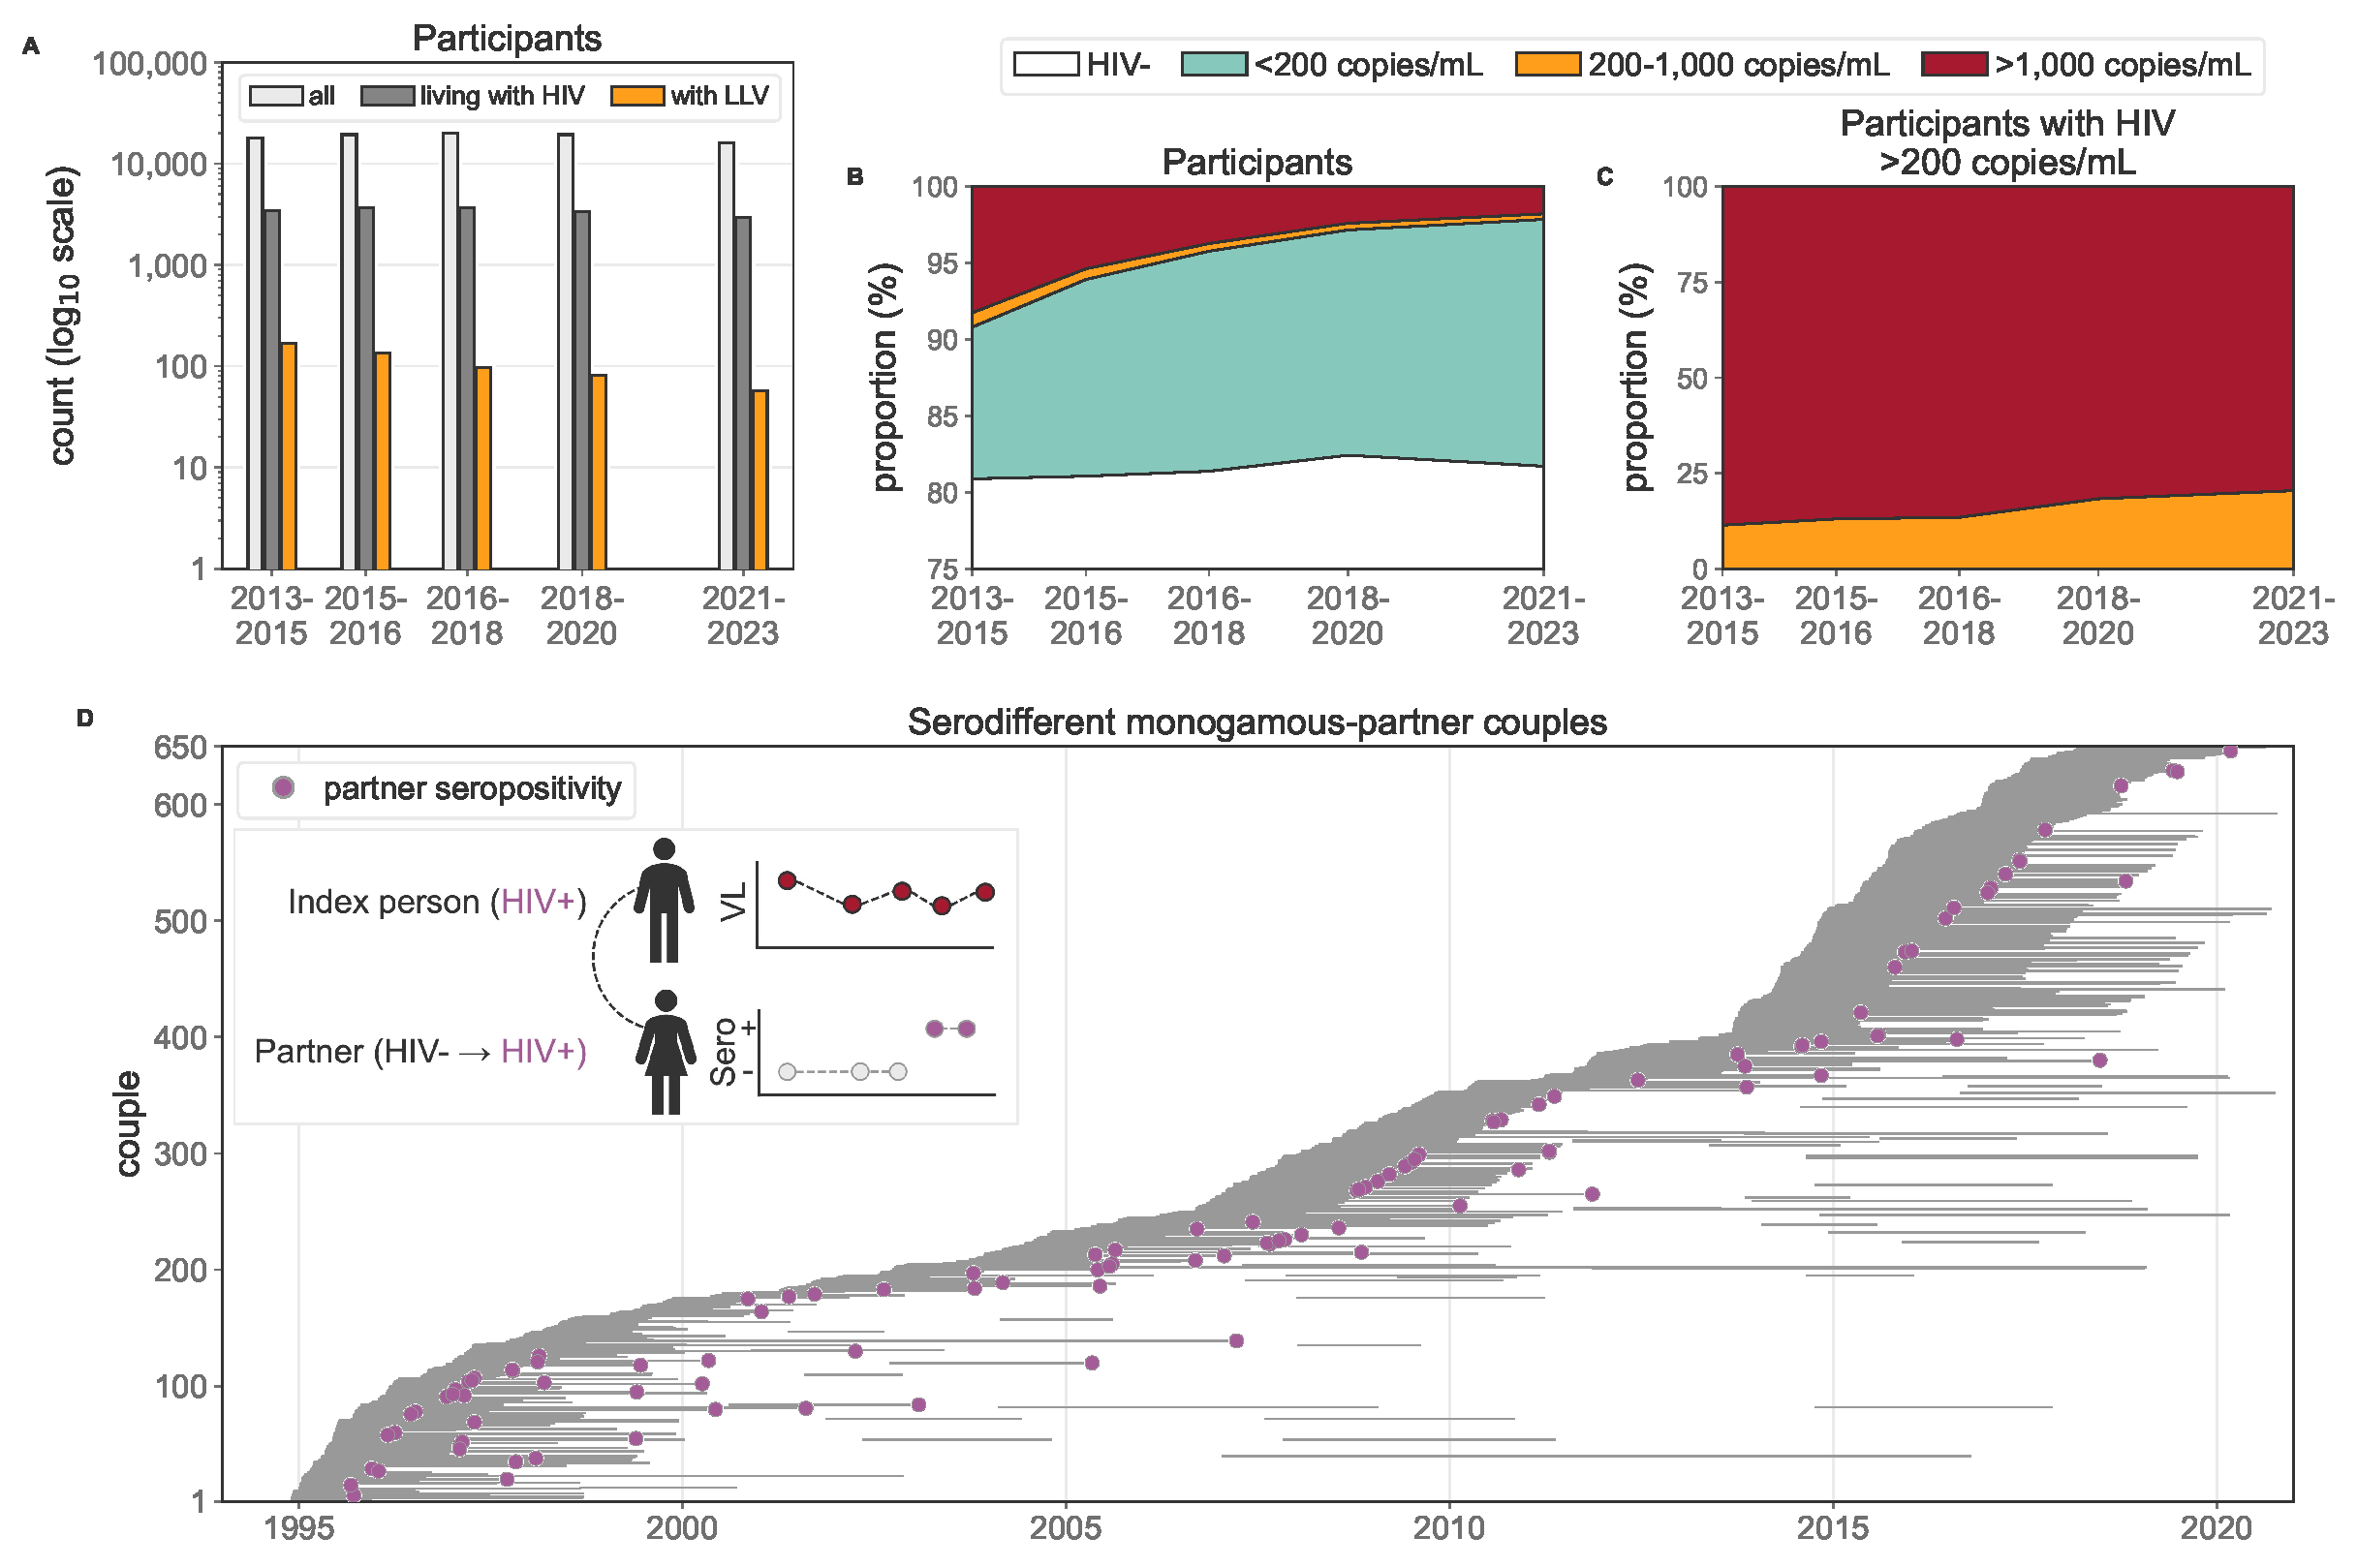
\includegraphics[width=1.0\textwidth]{../figures/eps/study_participants.eps}
    \caption{\protect \textbf{Participants in the Rakai Community Cohort Study (RCCS), \var{r1_medianYear}-\var{r20_medianYear}.} (A-C) Population-level trends from RCCS surveys conducted from \protect \var{r16_medianYear} onward in which viral load testing was performed for all participants with HIV. A) Number of (from left-to-right) participants, participants with HIV, and participants with low-level viremia (200-1,000 copies/mL) in each RCCS survey. B) Proportion of  RCCS participants with viremia ($>200$ copies/mL) who had low-level viremia in the same surveys. C) Proportion of all RCCS participants in these surveys who were (from bottom-to-top) HIV seronegative (HIV-) and HIV seropositive with viral load less than 40 copies/mL, between 40 and 200 copies/mL, between 200 and 1,000 copies/mL (low-level viremia) and $>1,000$ copies/mL. Y-axis truncated at 75\% for visual clarity. D) Periods of partnership (horizontal lines) among monogamous serodifferent couples with available index viral load data. First observation of HIV seropositivity in the initially seronegative partner indicated by points. Inset: Summary of couple sampling strategy.  
    }
    \label{fig:study_participants} % Used for referencing
\end{figure}


% ------- %
% REUSLTS %
% ------- %
\section*{Results}
\subsection*{Low-level viremia in the RCCS and serodifferent couple follow-up}

Between \var{r1_minDate} and \var{r20_maxDate}, \var{n_par} individuals participated in the Rakai Community Cohort Study (RCSS) including \var{n_plhiv} people with HIV. Prior to \var{r16_minDate}, viral load testing was conducted for a subset of participants with HIV, after which testing was expanded to all participants with HIV (\textbf{Figure \ref{fig:study_participants}A}). Of \var{n_plhiv_r16_plus} participants living with HIV during this period, \var{n_llv_r16_plus} (\var{p_llv_r16_plus}) had at least one viral load measurement between 200 and 1,000 copies/mL (LLV). Among participants with viremia  ($>200$ copies/ml), the estimated prevalence of LLV increased from  \var{q0.5_r16_200_1000_copies_prev_among_viremic} (95\% CI: \var{q0.025_r16_200_1000_copies_prev_among_viremic}, \var{q0.975_r16_200_1000_copies_prev_among_viremic}, unadjusted $n = $ \var{n_r16_llv}/\var{n_r16_viremic}) in \var{r16_medianYear} to \var{q0.5_r20_200_1000_copies_prev_among_viremic} in \var{r20_medianYear} (95\% CI: \var{q0.025_r20_200_1000_copies_prev_among_viremic}, \var{q0.975_r20_200_1000_copies_prev_among_viremic}, unadjusted $n = $ \var{n_r20_llv}/\var{n_r20_viremic}), after adjustment for \var{p_missing_vl_r16_plus} of missing viral load measurements and repeated observations (\textbf{Figure \ref{fig:study_participants}B}, \textbf{Supplementary Text}). In contrast, the overall population prevalence of LLV declined from \var{q0.5_r16_200_1000_copies_prev_among_par} (95\% CI: \var{q0.025_r16_200_1000_copies_prev_among_par}-\var{q0.975_r16_200_1000_copies_prev_among_par}, $n = $ \var{n_r16_llv}/\var{n_r16_par}) to \var{q0.5_r20_200_1000_copies_prev_among_par} (95\% CI: \var{q0.025_r20_200_1000_copies_prev_among_par}-\var{q0.975_r20_200_1000_copies_prev_among_par}, $n = $ \var{n_r20_llv}/\var{n_r20_par}) over this period due to increasing ART uptake and viral suppression (\textbf{Figure \ref{fig:study_participants}C}).

Because estimation of HIV transmission risk requires longitudinal follow-up of  HIV-seronegative persons exposed to HIV within a partnership, we restricted our  subsequent analyses to serodifferent couples. To minimize misclassification of infections acquired outside the partnership as within-partnership transmission events, we further limited analyses to couples reporting monogamy.  Between \var{r1_medianYear} and \var{r19_medianYear},   \var{n_donor-all_recipient-all_couples} serodifferent couples contributed at least one interval of follow-up between consecutive RCCS rounds, and of these \var{n_donor-all_recipient-exclusivelymonogamous_couples} included a  seronegative partner who reported monogamy (\textbf{Figure \ref{fig:study_participants}D}). Of these, \var{n_merged_donor-noacute_recipient-exclusivelymonogamous_couples} also had available index partner viral load data taken within two-years of the follow-up period used to assess HIV transmission and were greater than 180 days from observed seroconversion and were therefore included in the transmission analysis. Index partners in serodifferent couples, regardless of monogamy requirements, were more likely to be male, residing in agrarian communities, and 25 years old or older compared to all people with HIV over the same period
(\textbf{Table \ref{table:demograhics}}). As compared to all serodifferent couples, those with monogamous seronegative partners were less likely to have female index partners as men were more likely to report multiple partners. Each couple contributed a median of  \var{q050_merged_donor-noacute_recipient-exclusivelymonogamous_years} (range: \var{q000_merged_donor-noacute_recipient-exclusivelymonogamous_years}, \var{q100_merged_donor-noacute_recipient-exclusivelymonogamous_years}) couple-years of follow-up for a total of \var{n_merged_donor-noacute_recipient-exclusivelymonogamous_years} couple-years. Seronegative partner HIV testing was conducted at RCCS surveys and occurred every \var{q050_merged_donor-noacute_recipient-exclusivelymonogamous_interval} (range: \var{q000_merged_donor-noacute_recipient-exclusivelymonogamous_interval}, \var{q100_merged_donor-noacute_recipient-exclusivelymonogamous_interval}) years for seroengative partners in the \var{n_merged_donor-noacute_recipient-exclusivelymonogamous_couples} couples. Across all partnership periods the median duration between follow-up partner HIV testing and index viral load monitoring was \var{q050_merged_donor-noacute_recipient-exclusivelymonogamous_vl_testing_interval} (range: \var{q000_merged_donor-noacute_recipient-exclusivelymonogamous_vl_testing_interval}, \var{q100_merged_donor-noacute_recipient-exclusivelymonogamous_vl_testing_interval}) years.  

\begin{table}[htbp]
\centering
\caption{\textbf{Demographic characteristics of Rakai Community Cohort Study (RCCS) participants with HIV and index partners in monogamous serodifferent relationships, \var{r1_medianYear}-\var{r20_medianYear}.} Among all participants with HIV, age is reported as the median across  seropositive survey  visits. Among index partners in couples, age is reported as the age at the end of the partnership interval, taking the median of those ages when a given couple contributes multiple partnership intervals. Transmission analysis was restricted to monogamous couples in which the seropositive partner had available viral load measurements within two years of the follow-up period used to assess HIV transmission and excludes any couples in which the index partner was within 180 days of observed seroconversion.
\newline }
\begin{footnotesize}
\var{demographic_table}
\end{footnotesize}
\label{table:demograhics}
\end{table}



\subsection*{HIV seroconversions among partners in monogamous serodifferent couples}
\begin{table}
\centering
\caption{\textbf{Viral load trajectories of index partners in monogamous serodifferent partnerships proximal to the interval during which partner seroconversion occurred.} Viral loads have been rounded to the nearest hundred copies/mL for anonymization. Unavailable linkage data is due to missing viral genomic data for one or both partners in a given region.}
\footnotesize
\var{llv_table}
\label{table:llv}
\end{table}

Over \var{n_merged_donor-noacute_recipient-exclusivelymonogamous_years} couple-years of follow-up, \var{n_merged_donor-noacute_recipient-exclusivelymonogamous_seroconversion} initially seronegative partners seroconverted (\textbf{Figure \ref{fig:study_participants}D} and \textbf{Table \ref{table:demograhics}}). Index partners with seroconverting partners were demographically comparable to those with non-seroconverting partners. A total of \var{n_merged_donor-noacute_recipient-exclusivelymonogamous_llv_seroconversion} seroconversions were observed over \var{n_merged_donor-noacute_recipient-exclusivelymonogamous_llv_years} couple-years of follow-up contributed by \var{n_merged_donor-noacute_recipient-exclusivelymonogamous_llv_couples} couples in which the index partner had LLV in either the viral load measurement immediately preceding or following the interval during which the seronegative partner acquired HIV  (\textbf{Table \ref{table:llv}} and \textbf{Figure \ref{fig:select_vl_traj}}). Of \var{n_merged_donor-noacute_recipient-exclusivelymonogamous_llv_tx_200-1000_to_any_couples} couples in which the index partner had low-level viremia and self-reported treatment immediately prior to seroconversion,  \var{n_merged_donor-noacute_recipient-exclusivelymonogamous_llv_tx_200-1000_to_any_seroconversion} seroconverted. Quantifying the rate of intra-partner transmission based on these observed seroconversions, however, requires accounting for the probability of extra-partner transmission, all index viral load measurements taken proximal to a given transmission event, and the underlying functional shape of the relationship between viral load and transmission risk. 



\subsection*{Viral genetic linkage of intra-couple HIV transmissions}
To disentangle extra-couple acquisition from intra-couple transmission, we used HIV genetic sequence data generated as part of this study together with available sequence data from prior RCCS studies. Sequences from the  p24 (\textit{gag}) and gp41 (\textit{pol}) regions of the HIV-1 genome were used to assess genetic linkage between index-parter pairs. Pairs harboring viral genomes closely related by genetic distance (\var{p24_cutoff} [p24] and \var{gp41_cutoff} [gp41] substitutions per site) and phylogenetic topology (\textbf{Supplementary Text}) in at least one segment were considered linked. Genetic data in at least one segment were available for \var{n_couple_linkage_dat} couples (\var{p_couple_linkage_dat}) of which \var{n_couple_linked} were linked (\var{p_couple_linked}, \textbf{Figures \ref{fig:genetic_linkage}A} and \textbf{\ref{fig:genetic_linkage_distr}}). Of the \var{n_merged_donor-noacute_recipient-exclusivelymonogamous_llv_seroconversion} seroconverting LLV couples, linkage data were available for \var{n_llv_linkage_dat} of which \var{n_llv_linked_both} pairs were linked in both segments, suggesting a high-likelihood of intra-couple transmisison (\textbf{Figure \ref{fig:genetic_linkage}B,C,E,F} and \textbf{Table \ref{table:llv}}). Further, \var{n_llv_linked_only_gp41} were linked in gp41 but either lacked data or were unlinked in p24.  In a sixth couple, linkage data was only available in gp41 and genetic divergence was marginally higher than our empirically-determined threshold (\var{R78014_R04130_gp41_d_min} substitutions per site). However, tips from the index and seroconverting partners were monophyletic in this region and were both sampled about three years post partner seroconversion, suggesting likely transmission (\textbf{Figures \ref{fig:genetic_linkage}G} and \ref{fig:full_trees}). The remaining LLV seroconversion with genetic data was unambiguously unlinked. 

\begin{figure}[htbp] % h! forces the figure to stay "here"
    \centering
    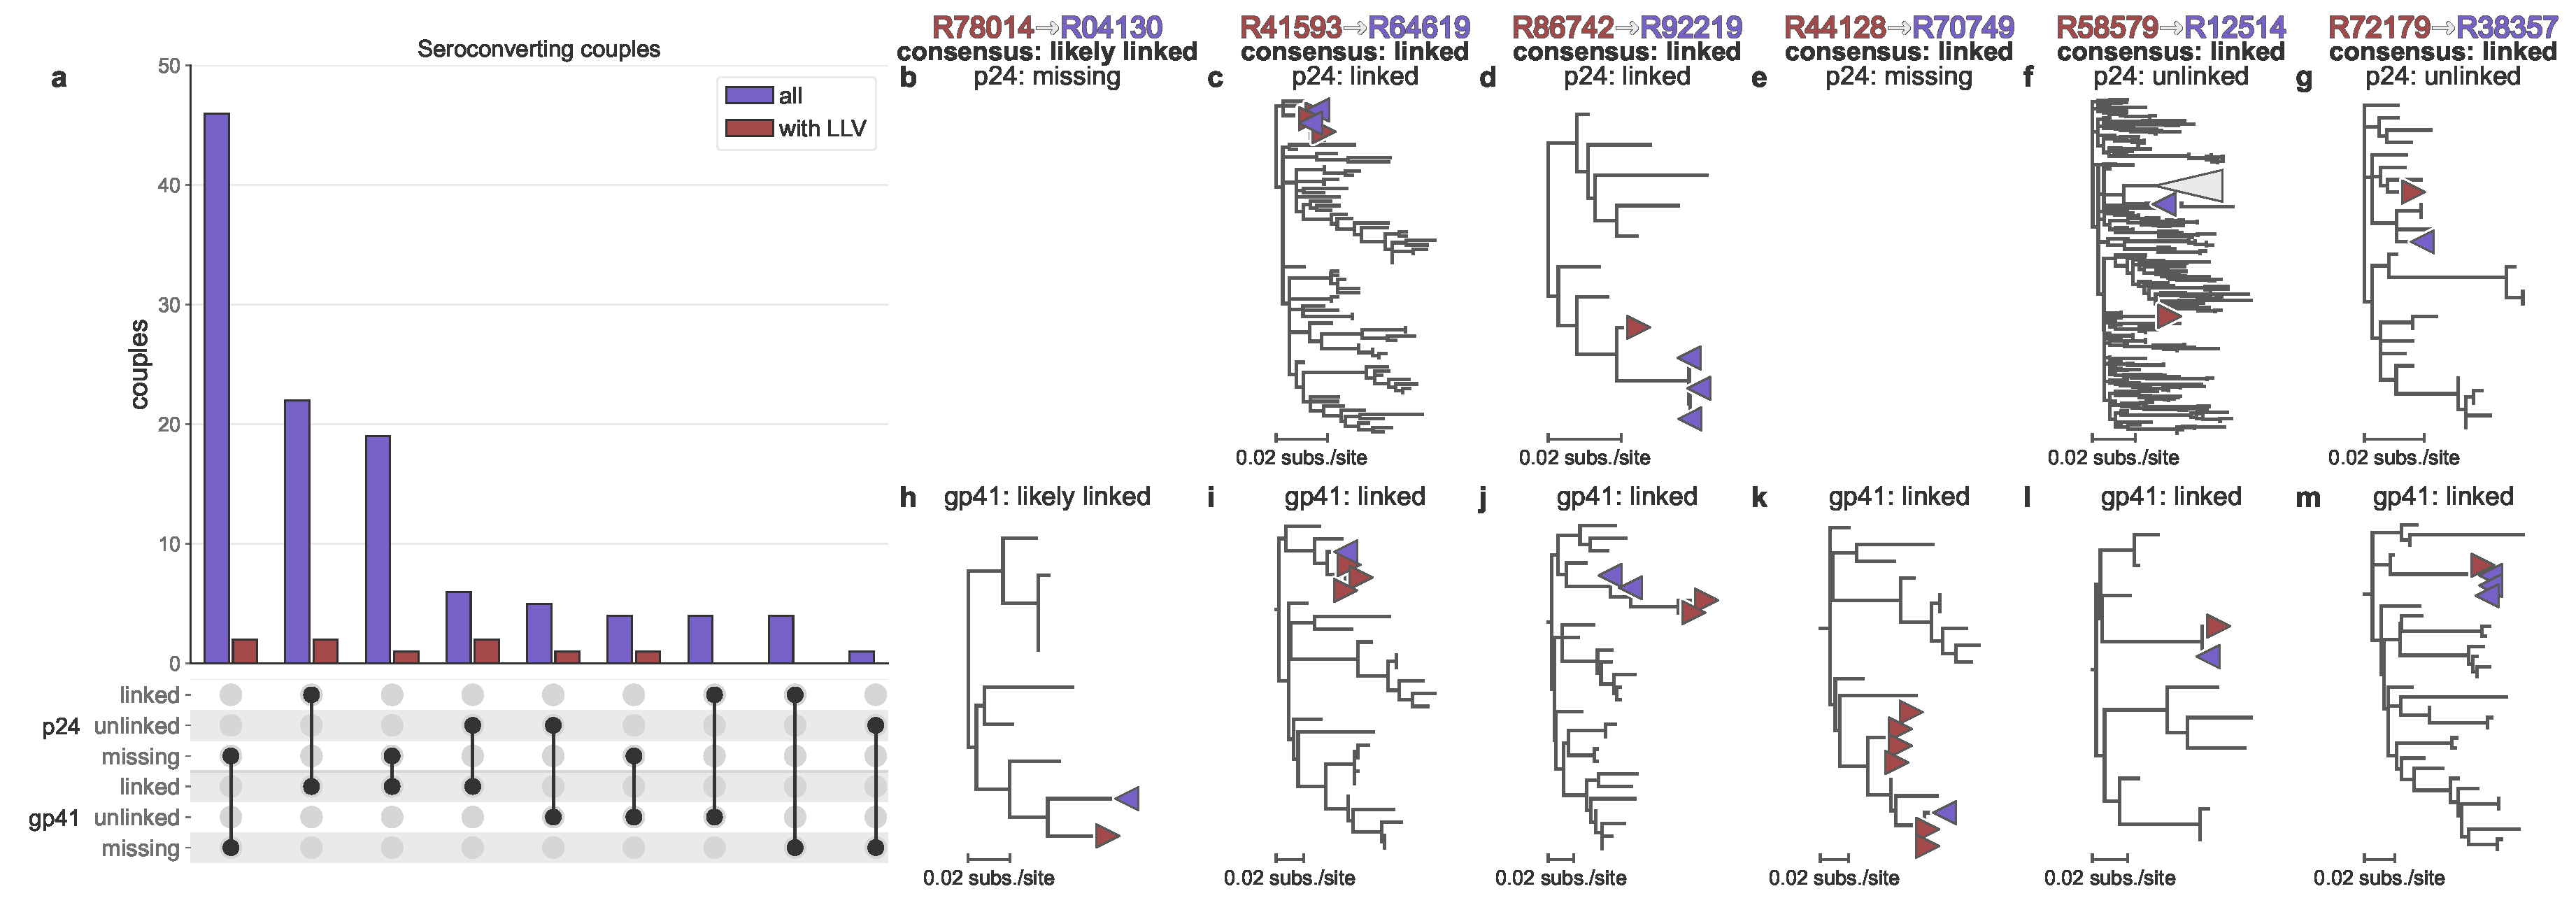
\includegraphics[width=1.0\textwidth]{../figures/eps/genetic_linkage.eps}
    \caption{\protect \textbf{Genetic linkage among HIV seroconversions in  monogamous serodifferent couples, Rakai Community Cohort Study (RCCS), \var{r1_minYear}-\var{r19_maxYear}.} A) Histogram of viral genetic linkage results for p24 (\textit{gag}) and gp41 (\textit{pol}) regions of the HIV-1 genome for observed seroconversions in all monogamous serodifferent couples (left) and in those in which the index partner had low-level viremia (right). (B-M) Couple phylogenetic subtrees in p24 (B-G) and gp41 (H-M) for index partners with low-level viremia and putative linkage. Subtrees the phylogenetic clade defined by the great grandparent of the index-partner common ancestor. Any clades with more than 100 tips not include one from the focal couple were collapsed and shown as grey triangles. Tips from index partners shown in right-facing arrows and tips from recipient partners show in left-facing arrows. Unlabelled tips are from other RCCS study participants. Consensus linkage determined by linkage either in p24 or gp41.}
    \label{fig:genetic_linkage} 
\end{figure}


\subsection*{Rate of intra-couple transmissions by index viral load}
To estimate the rate of transmission to seronegative partners as a function of index viral load, we developed a statistical model based on stochastic establishment of transmitted virions. This model incorporates the index partner viral load, a scaling factor to relate blood viral load to infectious dose per sexual act, a probability that any given transmitted virion establishes infection, the frequency of sexual acts, and the proportion of all sexual acts between serodifferent couples that can lead to transmission. The model also includes a constant rate of extra-partner transmission, which is informed by the observed proportions of incident infections that were genetically linked. As input to the model, we used the most recent index viral load at each time point in a given partnership interval. Index viral load measurements that were below-detection prior to self-reported or unreported ART-initiation were probabilistically imputed from pre-treatment within-individual viral load distributions to account for potential false negative viral load test results. Model parameters were estimated from the data using Bayesian inference with diffuse priors. 

We estimate that the rate of intra-couple transmission is reduced at low-level viremia, relative to viral loads $>1,000$ copies/mL, but it is non-zero. From 200 to 1,000 copies/mL, the estimated transmission rate increased from \var{q0.5_main_analysis_200_trans_rate_per_100_year} (95\% CI: \var{q0.025_main_analysis_200_trans_rate_per_100_year}-\var{q0.975_main_analysis_200_trans_rate_per_100_year}) to \var{q0.5_main_analysis_1000_trans_rate_per_100_year} (95\% CI: \var{q0.025_main_analysis_1000_trans_rate_per_100_year}-\var{q0.975_main_analysis_1000_trans_rate_per_100_year}) transmissions per 100 person-years as compared to \var{q0.5_main_analysis_mu_trans_rate_per_100_year} (95\% CI: \var{q0.025_main_analysis_mu_trans_rate_per_100_year}-\var{q0.975_main_analysis_mu_trans_rate_per_100_year}) at the geometric mean pre-treatment viral load in this setting (\var{q50_main_analysis_mu0} copies/mL, \textbf{Figures \ref{fig:intra_couple_transmission}A,B} and \ref{fig:main_analysis_correlation}). The risk ratio of transmission at 200 and 1,000 copies/mL relative to the mean viral load in the absence of treatment was \var{q0.5_main_analysis_200_v_mu_trans_rr} (95\% CI: \var{q0.975_main_analysis_200_v_mu_trans_rr}-\var{q0.025_main_analysis_200_v_mu_trans_rr}) and \var{q0.5_main_analysis_1000_v_mu_trans_rr} (95\% CI: \var{q0.975_main_analysis_1000_v_mu_trans_rr}-\var{q0.025_main_analysis_1000_v_mu_trans_rr}), respectively. As in prior work \cite{fraser2007, blanquart2016}, we estimate a saturating relationship between viral load and transmission rate, with a maximum estimated rate of \var{q0.5_main_analysis_max_trans_rate_per_100_year} (95\% CI: \var{q0.025_main_analysis_max_trans_rate_per_100_year}-\var{q0.975_main_analysis_max_trans_rate_per_100_year}) transmissions per 100 person-years. 
The rate of extra-partner transmission was estimated to be \var{q0.5_main_analysis_extra_trans_rate_per_100_year} (95\% CI: \var{q0.025_main_analysis_extra_trans_rate_per_100_year}-\var{q0.975_main_analysis_extra_trans_rate_per_100_year}) transmissions per 100 person-years. The risk of intra-couple transmission therefore reaches parity with that of extra-couple transmission  at a viral load of \var{q0.5_main_analysis_intra_extra_rr_parity} copies/mL (\textbf{Figure \ref{fig:intra_couple_transmission}C}). When incorporating index partner sex as a predictor of the transmission rate, we found that the median rate of male to female transitions is faster than vice versa throughout the viral load range, however, the 95\% CIs overlapped at all viral loads. Specifically at 1,000 copies/mL, the transmission rate from male index partners was    estimated to be \var{q0.5_sex_predictor_male_1000_trans_rate_per_100_year} (95\% CI: \var{q0.025_sex_predictor_male_1000_trans_rate_per_100_year}, \var{q0.975_sex_predictor_male_1000_trans_rate_per_100_year}) transmissions per 100 person-years as compared to \var{q0.5_sex_predictor_female_1000_trans_rate_per_100_year} (95\% CI: \var{q0.025_sex_predictor_female_1000_trans_rate_per_100_year}, \var{q0.975_sex_predictor_female_1000_trans_rate_per_100_year}) from female index partners (\textbf{Figure \ref{fig:intra_couple_trans_risk_all}}). Unsurprisingly, the estimated transmission rate at LLV was about two-fold higher when not accounting for genetic linkage but was otherwise relatively robust, given the wide confidence bounds, to sensitivity analyses accounting for assumptions about the genetically informed prior on the extra-partner transmission rate, the true value of undetectable viral loads due to treatment, and the inclusion only of index partners who were not yet on treatment (\textbf{Figures \ref{fig:est_c_correlation}} and \ref{fig:intra_couple_trans_risk_all} and \textbf{Tables} \ref{table:fit_vl_params}, \ref{table:fit_bd_params}, and \ref{table:fit_rates}). 

We also evaluated the sensitivity of our key inferences to assumptions about the functional form of the relationship between index viral load and rate of heterosexual HIV transmission. An alternative functional form with the proportion of all sexual acts that can lead to transmission fixed at 1 produced a significantly worse fit to the data as measured by leave-one-out cross-validation, confirming that the saturating relationship observed in the main analysis is strongly supported by the data (LOO CV, \textbf{Figure \ref{fig:intra_couple_trans_risk_all}} and \textbf{Table \ref{table:fit_compare}}). The estimated transmission rate within LLV was slightly higher, although not significantly different, when using a sigmoidal (also known as Hill) functional form as in previous studies \cite{blanquart2016, fraser2007} (\textbf{Figure \ref{fig:intra_couple_trans_risk_all}} and \textbf{Table \ref{table:fit_rates}}), which had comparable predictive performance to the virion establishment model (\textbf{Table \ref{table:fit_compare}}). We therefore chose to use the virion establishment model for the remainder of our analyses as it scales transmission risk across the full range of viral load values in a biologically grounded, as opposed to purely statistical, manner. 

\begin{figure}[htbp] 
    \centering
    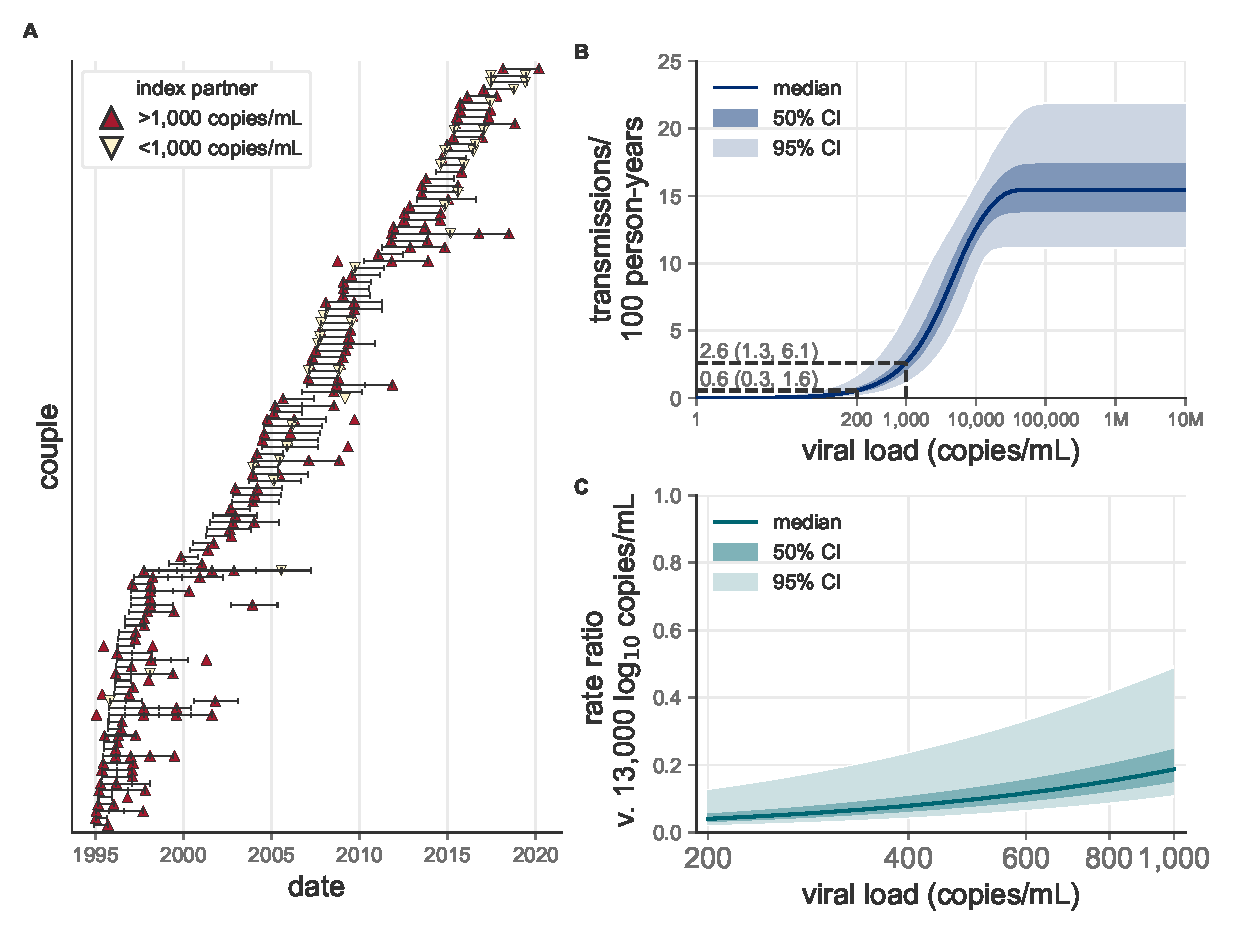
\includegraphics[width=1.0\textwidth]{../figures/eps/intra_couple_transmission.eps}
    \caption{\protect \textbf{HIV transmission in monogamous serodifferent couples, Rakai Community Cohort Study, \var{r1_minYear}-\var{r19_maxYear}.} A) Periods of partnership between monogamous serodifferent couples in which partner seroconversion was observed. Contiguous horizontal lines represent periods of monogamous partnership and vertical lines indicate timing of HIV testing of the initially seronegative partner. All periods are truncated at the date of the initially seronegative partner's first seropositive test result. Index partner viral load shown in filled circules. B) Estimated transmission rate per 100 person-years as a function of index partner viral load. Dotted lines highlight the risk of transmission among donors with low-level viremia (200-1,000 copies/mL). C) Risk ratio of intra-couple to extra-couple transmission at selected viral loads. Dotted horizontal line at 1 indicates parity between intra- and extra-couple transmission rates. Y-axis truncated at 7 for visual clarity. (B,C) Median value is shown as the central line and shading represents the 95\% and 50\% credible interval. }
    \label{fig:intra_couple_transmission} 
\end{figure}


\subsection*{Stability of low-level viremia among participants on treatment}

Individual-level HIV viral load among those on treatment can change rapidly based on patterns of treatment adherence and the emergence of resistance. To quantify the stability of low-level viremia among participants self-reporting treatment, we used paired viral load measurements from consecutive surveys from \var{n_uniq_tx_llv_vl_pairs} individuals with low-level viremia. 
After a median of \var{q050_uniq_tx_llv_vl_pairs_years} (95th percentile \var{q025_uniq_tx_llv_vl_pairs_years}-\var{q975_uniq_tx_llv_vl_pairs_years}) years, only \var{n_uniq_tx_llv_vl_pairs_200_to_1000_copies} participants (\var{p_uniq_tx_llv_vl_pairs_200_to_1000_copies}) remained at low-level viremia. While most ($n=$ \var{n_uniq_tx_llv_vl_pairs_0_to_40_copies}, \var{p_uniq_tx_llv_vl_pairs_0_to_40_copies}) individuals went on to achieve undetectable viral loads, \var{n_uniq_tx_llv_vl_pairs_1000_to_inf_copies} (\var{p_uniq_tx_llv_vl_pairs_1000_to_inf_copies}) rebounded to $>1,000$ copies/mL by the time of follow-up (\textbf{Figure \ref{fig:vl_traj}A}). In sharp contrast, among \var{n_uniq_tx_supr_vl_pairs} individuals with below-detection viral loads, nearly all ($n=$ \var{n_uniq_tx_supr_vl_pairs_0_to_40_copies}, \var{p_uniq_tx_supr_vl_pairs_0_to_40_copies}) remained suppressed at the subsequent survey (\textbf{Figure \ref{fig:vl_traj}B}). These results indicate that, in contrast to viral load suppression, LLV in real-world settings is a highly dynamic state and quantifying the positive predictive value of measured LLV with regards to future transmission risk must account for these dynamics. 

\begin{figure}[htbp] 
    \centering
    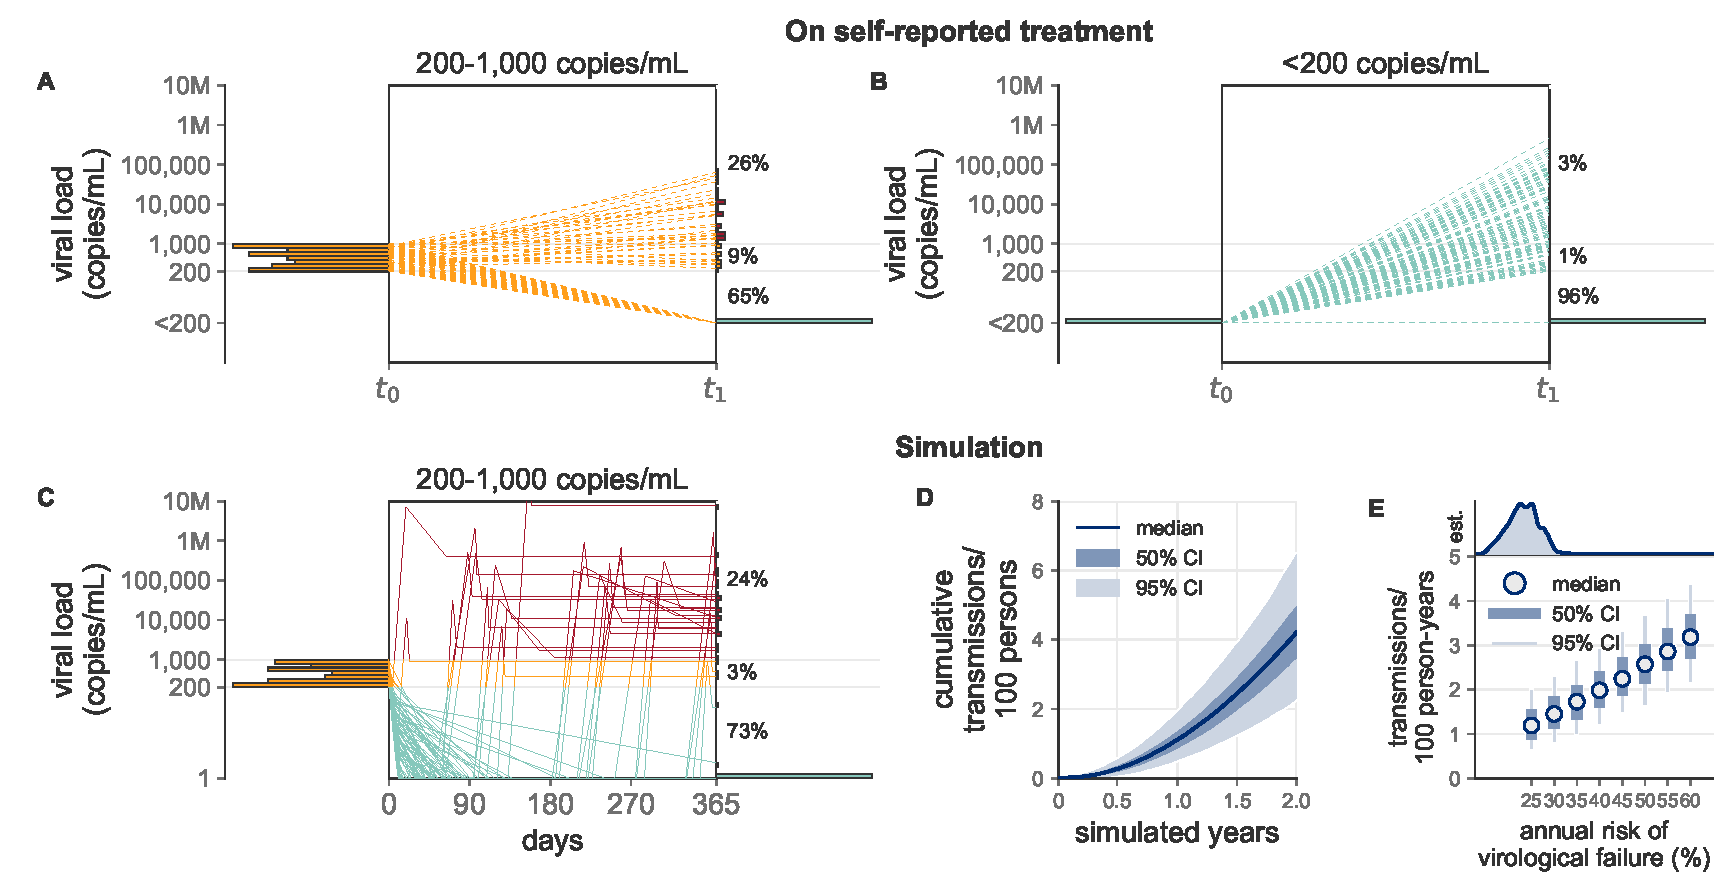
\includegraphics[width=1.0\textwidth]{../figures/eps/vl_trajs.eps}
    \caption{\protect \textbf{HIV viral load trajectories among Rakai Community Cohort Study (RCCS) participants on antiretroviral therapy (ART), \var{r1_minYear}-\var{r20_maxYear}.} (A-B) Paired viral load measurements from consecutive RCCS surveys from individuals self reporting ART use with viral low-level viremia (200-1,000 copies/mL), (A) and viral load suppression ($<40$ copies/mL) (B) at the initial survey round. Horizontal histograms show the distribution of viral loads in the initial and follow-up surveys and the proportion of follow-up viral loads that are $<40$, 40-200, 200-1,000 and $>1,000$ copies/mL are annotated on the follow-up histogram. Dashed lines connect measurements from the same participant, but do not represent intra-observation viral load dynamics. Includes only the first available pair per-participant within each category. C) Representative simulated viral load trajectories over a one year period of 100 individuals on treatment at time 0 with a constant rate of rebound calibrated to the trajectories in (A). D) Estimated cumulative transmissions from 100 individuals on treatment and with low-level viremia at baseline at each time point over a two-year period using rebound rate calibrated to the trajectories in (A). Shading extends from the 2.5th to the 97.5th percentile and the 25th to the 75th percentile and the central estimate is the 50th percentile. Y-axis is truncated at 1.4 transmissions per 100 persons for visual clarity. E) Estimated risk of transmission from 100 individuals on treatment and with low-level viremia at time 0 over a one year period across fixed rebound rates. Central estimate is the median and whiskers extend to the 50\% and 95\% credible interval. Density plot shows estimated rebound rate based on the trajectories in (A).}
    \label{fig:vl_traj} % Used for referencing
\end{figure}

To account for these patterns, we calibrated an individual-level model of treatment adherence and subsequent viral load dynamics. We simulated viral load dynamics among a cohort of individuals with LLV who are on effective treatment at baseline and have a time-homogeneous rate of treatment cessation or resistance emergence resulting in virological failure (i.e., follow-up viral load $>1,000$ copies/mL) over a two year period (\textbf{Figures \ref{fig:vl_traj}C}). We estimate the rate of treatment cessation or resistance emergence among RCCCS participants with low-level viremia to be \var{q0.5_omega_cease_per_year} (95\% CI: \var{q0.025_omega_cease_per_year}, \var{q0.975_omega_cease_per_year}) per year, translating to a median annual probability of cessation or resistance of \var{q0.5_risk_failure_per_year}\% (95\% CI: \var{q0.025_risk_failure_per_year}\%-\var{q0.975_risk_failure_per_year}\%). The transmission risk for these simulated viral load trajectories was calculated using the relationship estimated here (\textbf{Figure \ref{fig:intra_couple_transmission}A}). We expect \var{q0.5_sampled_trans_risk_1yr} (95\% CI: \var{q0.025_sampled_trans_risk_1yr}-\var{q0.975_sampled_trans_risk_1yr}) transmissions per 100 person-years to arise from this cohort in the first year after low-level viremia (\textbf{Figure \ref{fig:vl_traj}D}). Because most with LLV achieve suppression at follow-up, this risk is less than that at 1,000 copies/mL. However, given the exponential increase in transmission rate within this viral load range, \var{q0.5_prop_trans_risk_rebounded_1yr} (95\% CI: \var{q0.025_prop_trans_risk_rebounded_1yr}-\var{q0.975_prop_trans_risk_rebounded_1yr}) of transmissions in this simulated cohort at one year were contributed by the \var{q0.5_prop_rebounded_1yr} (95\% CI: \var{q0.025_prop_rebounded_1yr}-\var{q0.975_prop_rebounded_1yr}) of simulated people with viral load rebound ($>1,000$ copies/mL at follow-up) after one year. Moreover, under a constant rate of treatment cessation during follow-up, cumulative transmission risk increased in a non-linear fashion: only \var{q0.5_prop_trans_risk_90} (95\% CI: \var{q0.025_prop_trans_risk_90}-\var{q0.975_prop_trans_risk_90}) of the cumulative annual risk occurred within the first 90 days (\textbf{Figure \ref{fig:vl_traj}D}). Similarly, in the absence of any viral load monitoring in the interim to affect individual-level patterns of adherence we expect that by two years following measured low-level viremia we expect a total of \var{q0.5_sampled_trans_risk_2yr} (95\% CI: \var{q0.025_sampled_trans_risk_2yr}, \var{q0.975_sampled_trans_risk_2yr}) transmissions per 100 persons. This suggests a potential utility for more frequent viral load monitoring to rapidly identify and intervene on those individuals with virological failure following LLV.   

Observed viral load trajectories were collected during rapid treatment scale-up and increased rates of viral suppression among people with HIV \cite{grabowski2017, martin2026}. Given that ongoing reductions in global funding for HIV treatment and care   may result in increased rates of virological failure among people with HIV \cite{brink2025}, including those with LLV, we also simulated additional cohorts with annual probabilities of virological failure ranging from 25\% (comparable to the observed probability of \var{q0.5_risk_failure_per_year}\%) to 65\%. A modest increase in cessation probability from  25\% to 30\% per year translates to an increase from \var{q0.5_0.0007881700615_fixed_trans_risk} (95\% CI: \var{q0.025_0.0007881700615_fixed_trans_risk}-\var{q0.975_0.0007881700615_fixed_trans_risk} to \var{q0.5_0.00097719_fixed_trans_risk} (95\% CI: \var{q0.025_0.00097719_fixed_trans_risk}-\var{q0.975_0.00097719_fixed_trans_risk}.
%\var{q0.5_0.00097719_fixed_trans_risk} (95\% CI: \var{q0.025_0.00097719_fixed_trans_risk}-\var{q0.975_0.00097719_fixed_trans_risk}) to \var{q0.5_0.00118023_fixed_trans_risk} (95\% CI: \var{q0.025_0.00118023_fixed_trans_risk}-\var{q0.975_0.00118023_fixed_trans_risk}) transmissions per 100 person-years (\textbf{Figure \ref{fig:vl_traj}E}).
At the upper-bound of our simulated range, we expect as many as \var{q0.5_0.00251039_fixed_trans_risk} (95\% CI: \var{q0.025_0.00251039_fixed_trans_risk}-\var{q0.975_0.00251039_fixed_trans_risk}) transmissions per 100 person-years. Taken together, this highlights the fact that given the observed instability of LLV, the expected transmission risk from people with LLV between viral load monitoring events depends on the rate of virological failure, as determined by setting-specific individual (e.g. adherence) and exogenous (e.g. access) factors. 

\section*{Discussion}
In this study we used real-world data to estimate the rate of heterosexual HIV transmission at low-level viremia (LLV, 200-1,000 copies/mL) and to quantify the uncertainty in these estimates based on available data. We observed \var{n_llv_likely_linked} likely linked transmissions from individuals with LLV and show that the rate of transmissions at LLV ranges from \var{q0.5_main_analysis_200_v_mu_trans_rr_percent} (at 200 copies/mL) to \var{q0.5_main_analysis_1000_v_mu_trans_rr_percent} (1,000 copies/mL) of that at mean untreated viral loads. We further showed that LLV while on treatment is a highly unstable state, with only \var{p_uniq_tx_llv_vl_pairs_200_to_1000_copies}\% of people remaining at LLV between monitoring events. After accounting for this instability, we expect \var{q0.5_sampled_trans_risk_1yr} transmissions per 100 person-years to arise from a cohort of treated individuals with LLV at current rates of viral load rebound. These findings provide critical context to our understanding of the real-world risk of HIV transmission in this VL range and support public health guidance and individual-level decision making. 

This work is particularly salient given WHO policy that aggregates the risk of HIV transmission for all individuals with detectable viral loads $<1,000$ copies/mL based on a qualitative systematic review that concluded there to be an ``almost zero'' risk of sexual HIV transmission within LLV \cite{broyles2023}. Despite this conclusion, two instances of genetically linked intra-couple transmissions were reported in this review: one out of the eight post-ART initiation linked transmissions in HPTN052 and one out of three in Partners PrEP \cite{cohen2016, mujugira2016}, which suggests that some transmission risk persists within this range. While viral loads for these two cases were taken 50 and 53 days prior to partner seroconversion, this is far more frequent than viral load monitoring is accessed in real-world settings, particularly in sub-Saharan Africa \cite{kippen2024}. Further, quantifying the transmission risk from observed linked infections requires data on couple-years of follow-up among seroconverting and non-seroconverting couples, which is not readily available for the aforementioned studies, and defining a statistical model for the relationship between viral load and transmission rate, as we have done here. 

Our work follows previous efforts to relate HIV index partner viral load to transmission using longitudinal follow-up of serodifferent couples in this same cohort \cite{fraser2007, quinn2000, blanquart2016}. Our results are consistent with prior findings demonstrating a reduced, but non-zero, risk of transmission at viral loads between 200 and 1,000 copies/mL \cite{blanquart2016}. Here, we utilized an additional decade of follow-up, supporting strict monogamy and linkage thresholds while retaining statistical power. We also developed a novel statistical model that allows us to use data across the range of observed viral loads to inform transmission at LLV in a biologically grounded manner and incorporated data on the time of viral load monitoring to estimate the relationship between proximal, as opposed to set-point, viral load and transmission rate. Consequently, we were able to explicitly link within-individual viral load dynamics with their risk of transmission, thereby accounting for viral rebounds in our understanding of transmission from individuals with LLV and  quantify transmission risk at LLV. 

Low-level viremia is most commonly associated with incomplete viral suppression on ART or with the rare ``viremic controller'' phenotype, which results in partial immunological control of virus in the absence of treatment \cite{okulicz_clinical_2009, kwaa_immune_2024}. However, suppressed but detectable viremia is also now considered by some to be an acceptable goal of HIV cure, as research has moved away from cure strategies aimed at completely preventing reactivation of latent virus and shifted towards boosting anti-viral immunity to achieve ``post-intervention control''\cite{gunst_time_2025, wagner_advances_2026}. Recent clinical trial results have demonstrated this possibility: In RIO trial of combination broadly neutralizing antibodies (bNAbs), 5/28 participants in Arm B maintained LLV for close to a year following cessation of all therapies \cite{edgar_abstract_2026}, and in another trial combining bNAbs, a TLR9 agonist, and therapeutic vaccination, 4/10 participants eventually suppressed rebounding virus to LLV levels for 3-5 months \cite{peluso_correlates_2026}. 
Although widely-available therapies to induce long-term HIV remission could be many years off, understanding transmission risk following ART cessation is critical to directing investment in this area, counseling participants in clinical trials, determining acceptable definitions of ``cure'', and eventually, understanding residual population risk of transmission. 

It is important to distinguish between the risk of transmission from an individual with LLV, which we estimate here, and the proportion of all HIV transmissions at the population level attributable to individuals with LLV. The former is most relevant for counseling individuals and informing clinical guidance, whereas the latter is more relevant for decisions regarding investments in viral load monitoring and testing technologies. Because individuals with LLV comprise a relatively small proportion of all viremic persons in sub-Saharan Africa, a prior modeling study estimated that LLV contributes little to overall HIV transmission \cite{larmarange2023}. However, that analysis treated viral load as a static characteristic and did not account for the dynamic nature of LLV. Consistent with previous studies \cite{nzivo2023, antiretroviraltherapycohort2015, laprise2013, fleming2019}, we found that individuals with LLV are at elevated risk of subsequent viral rebound as compared to those with detectable viral loads $<200$ copies/mL, suggesting that their cumulative contribution to transmission may be greater than would be predicted from a single viral load measurement alone. Although individuals with LLV may contribute relatively little to population-level transmission, our findings suggest that both assay sensitivity and testing frequency should be considered when interpreting viral load results and communicating transmission risk.

This analysis leverages data collected as part of an observational, population-based study over the past 30 years and is therefore subject to limitations inherent to observational data collected under real-world conditions.  Specifically, these data were collected in a heterosexual HIV epidemic dominated by subtype A1 and D viruses and our findings may not be generalizable to epidemics characterized by other transmission modes or viral genotypes. The intra-couple rate of HIV transmission is dependent on behavioral dynamics such as the frequency of sex, use of condoms, and treatment adherence that may differ in other settings. Further, as this general surveillance cohort was not designed specifically to answer this question, our study suffers from limitations of the study design, such as sparsity of viral load data prior to \var{r16_minYear}, relatively long durations between viral load monitoring and imperfect availability of genetic linkage data. Nevertheless, the longitudinal population-based sampling scheme employed in this study is necessary to understand how viral load and transmission are related while accounting for real-world behavioral and virological dynamics.   

As compared to people with undetectable HIV viral loads ($<200$ copies/mL), those with viral loads between 200 and 1,000 copies/mL are at elevated risk of future virological failure and, as we have shown here, transmission to seronegative partners. Moreover, there is a five-fold increase in the rate of transmission across LLV. Given these risks, quantitative viral load measurements within the detectable yet $<1,000$ copies/mL range may enable individuals to make informed decisions about treatment adherence and sexual behavior. Further, distinguishing individuals with LLV from those with detectable viral loads $<200$ copies/mL represents an opportunity for the healthcare and public health system to intervene to avert poor outcomes for individual health and incident HIV infections. 

\section*{Materials \& Methods}

Study methods are summarized here, with more details provided in the \textbf{Supplementary Text}.

\subsection*{Study participants and couple ascertainment}
The Rakai Community Cohort Study (RCCS) is a population-based census and open-cohort study that has been conducted every 18-24 months since \var{r1_minYear} in inland and Lake Victoria fishing communities in southern Uganda by the Rakai Health Sciences Program (Kalisizo, Uganda). During surveys participating communities are censused and residents aged 15-49 invited to participate in the study. The census records the composition and familial and spousal relationships among household members in participating communities, including the identification of cohabitating couples. Study participants complete structured questionnaires to obtain information on demographics, sexual behaviors, HIV testing history and ART use, and provide samples for HIV testing, viral load monitoring, and viral genetic sequencing. At time of survey, participants are also asked disclose the names of cohabitiating sexual partners . 

In this study, cohabitating couples were ascertained  using both the community census and reported spousal relationships at time of survey.  We considered an  initially HIV-negative participant in these couples to be monogamous in a given survey if they were in no more than one cohabitating partnership in the census, and reported no more than one sexual partner in the past year or more than one spouse at time of survey.  

Among serodifferent spousal partnerships (one HIV seropositive partner and one HIV seronegative partner) in which the seronegative partner was monogamous, we identified periods of coupling during which transmission could potentially have occurred. These periods are defined based on consecutive RCCS surveys during which the seronegative partner had available HIV testing results at both the preceding and the subsequent survey and reported monogamy at both surveys. The duration of each period was taken as the duration of calendar time between the survey dates for the initially seronegative partner. After identification of coupling periods, we subsetted to those in which the entire coupling period was within no more than two-years (approximately the duration between two RCCS surveys) of a viral load measurement for the seropositive partner. 

\subsection*{Viral load monitoring}
Viral load monitoring of all consenting HIV seropositive study participants has been conducted since the 16th survey round beginning on \var{r16_minDate}. Prior to this,  viral load monitoring for other Rakai Health Sciences Program research studies was conducted for a subset of study participants based on available funding. Viral load monitoring was conducted at either the Makerere University Walter Reed Project Laboratory (Kampala, Uganda), the International HIV and STD laboratory at
Johns Hopkins University (Baltimore, MD, USA), or the Rakai Health Sciences Program (RHSP, Kalisizo, Uganda) using either the Roche  Amplicor v1.5 (Walter Reed, Johns Hopkins, RHSP until Nov. 2010) or the Abbott Laboratories (Chicago, IL, USA) m2000 RealTime HIV-1 Quantitative PCR assay (RHSP, Oct. 2010 onward). No systematic differences were observed across assays \cite{blanquart2016}. 

\subsection*{Statistical model relating viral load to transmission rate}
To quantify the relationship between seropositive partner viral load and the rate of transmission to their seronegative partner, we developed a statistical model based on a per-virion stochastic establishment process. Specifically, we calculated the probability of intra-couple transmission occurring from individual $j$ to individual $i$ during interval $k$ ($y_{i,k}$) of duration $t_{i,k}$ years at an index partner viral load of $V_{j,k}$ copies/mL as:
\begin{equation}
P(y_{i,j,k}=1|t_{i,k},V_{j,k}) = 1-e^{- f t_{i,k} \rho_{\text{prod.}} \left(1-\left(1-\rho_{\text{est.}}\right)^{c V_{j,k}}\right) }
\end{equation}
where $\rho_{\text{est.}}$ is the probability of a single virion establishing infection during a sexual event amenable to transmission, $c$ is a constant of proportionality relating blood viral load to infectious dose during heterosexual intercourse, $\rho_{\text{prod.}}$ is the proportion of sexual acts amenable to transmission, and $f$ is the frequency of sex per year (taken to be 108 year$^{-1}$, \cite{gray2001}). To account for the probability of extra-couple transmission, we calculate the probability of partner seroconversion ($s_{i,j,k}$) as:
\begin{equation}
%P(s_{i,j,k}=1|t_{i,k},V_{j,k}) = 1-e^{-\beta_{\text{extra}}t_{i,k}}\left(1-P(y_{i,j,k}=1|t_{i,k},V_{j,k})\right),
P(s_{i,j,k}=1|t_{i,k},V_{j,k}, m_{i,j,k}=1) = 1-e^{-t_{i,k}\left[\beta_\text{extra} + f \rho_{\text{prod.}} \left(1-\left(1-\rho_{\text{est.}}\right)^{c V_{j,k}}\right) \right]}
\end{equation}
where $\beta_\text{extra}$ is the rate of extra-couple transmission in monogamous cohabitating (indicated by $m_{i,j,k}=1$) partnerships. Due to mutual non-identifiability of model parameters, we fix $c=1$, which was shown to negligibly affect inferences as compared to using a mildly-informative prior on $c$. 

To incorporate information on genetic linkage, we set a prior distribution on $\beta_\text{extra}$ based on the proportion of observed transmissions with available genetic data that are inferred to be linked. 
 
Due to the spurious presence of below-detection viral loads prior to the availability of ART in this setting, we also accounted for the possibility of false-negative viral load measurements. In the era following ART introduction, we also accounted for the possibility of unreported ART use. To do so, we estimated the expected variation within and between individuals in pre-treatment (``set-point'') viral loads using a hierarchical model, which was informed by viral load measurements from all RCCS participants (not just monogamous serodifferent partners used in estimating transmission rates). These distributions were used to differentiate below-detection viral loads due to 1) true negatives due to intra-individual pre-treatment variability, 2) false negatives, and 3) true negatives due to unreported ART. True values for each scenario were estimated as free parameters in the model with the following constraints: 1) true negatives due to intra-individual variability followed the estimated pre-treatment viral load distributions right-truncated at the limit of detection, 2) false negatives followed the non-truncated expected pre-treatment distribution, and 3) true negatives due to unreported ART followed a uniform distribution between 0 and 40 copies/mL. 

The joint posterior of the transmission model and the intra-individual model of viral load variation was sampled using Hamiltonian Monte-Carlo as implement in \textsc{Stan} for \textsc{Python} (accessed through \textsc{CmdStanPy}) using four chains with 1,000 warm-up iterations and 1,000 sampling iterations. Diffuse priors were used for all parameters. Convergence was assessed using the $\hat{R}$ statistic, bulk and tail effective population sizes, and visual inspection of trace and pairs plots. Posterior distribution percentiles were used as credible intervals, e.g. the 95\% credible interval spans from the 2.5th posterior percentile to the 97.5th posterior percentile.  


\subsection*{Viral genetic sequencing and transmission linkage}
HIV-1 viral genetic sequencing was conducted using one of four protocols protocols \cite{kim2024}: 1) Sanger sequencing of the p24 (\textit{gag}, HXB2: 1249-1704) and gp41 (\textit{env}, HXB2: 7857-8260) regions (prior to 2010), 2) Illumina MiSeq and HiSeq next-generation sequencing (NGS) using an amplicon protocol \cite{gall2012}, 3) Illumina NoVaSeq NGS using a bait-capture protocol \cite{bonsall2020}, 4) Sanger single genome sequencing of p24 and gp41 using residual samples from participants in low-level viremia couples with observed seroconversions based on an adaptation of a recently developed protocol \cite{box2026}. NGS reads were assembled into consensus genomes using Shiver v.1.5.7. Consensus and Sanger sequences were aligned using \textsc{MAFFT} v.7.490 and trimmed to the p24 (HXB2: 1315-1701) and gp41 (HXB2: 7857-8258) regions to ensure completeness. Kimura 2-parameter distances were calculated between complete ($>$95\%) segment sequences and distance cut-offs selected via Youden's J comparing intra-individual distances to distances between random pairs. Phylogenetic trees were inferred using \textsc{IQ-Tree} v.2.2.2.7 and used to identify clustering patterns consistent with transmission (\textbf{Supplementary Text}). Sequences were considered linked in a given region if they were linked by both genetic distance and phylogenetic topology in that region. 


\subsection*{Simulation model of individual-level treatment adherence and viral dynamics}

We utilized a stochastic simulation-based framework to describe the process of ART adherence and cessation and subsequent viral load dynamics of people living with HIV, following a single measurement of low-level viremia (LLV). We utilized a previously-fit log-linear biphasic decay model to describe individual-level HIV viral load dynamics when on ART, calibrated to participants in a clinical trial of integrase-inhibitor-based treatment with frequent viral load sampling (ACTG A5248, \cite{andrade2013}). Viral rebound dynamics in the absence of treatment were modeled as a three-segment piecewise log-linear function with an initial growth period to the viral load peak followed by a decay to the viral set-point. Parameters for this model were fit to data from participants collected from three studies of supervised ART interruption with no additional interventions (ACTG A5024, A5068, and A5197, \cite{li_size_2016}) using a hierarchical model. 

Given these models of viral dynamics when on- and off antiretroviral therapy, we developed a stochastic, time-discrete model of individual-level treatment adherence and subsequent viral load dynamics. Individuals on treatment can cease treatment at a rate $\omega^{\text{cease}}$ per day, assumed to be constant across individuals and time. Viral load dynamics while on or off ART are assumed to be governed by the viral dynamics models described above. We first used this model to estimate the rate of treatment cessation ($\omega^{\text{cease}}$) based on paired viral load measurements in subsequent RCCS surveys from those who self-report treatment and have LLV at the preceding survey. We assume all individuals are actively on treatment at the initial survey. Model fitting was performed using Markov Chain Monte Carlo with 25,000 iterations, discarding the first 50\% as burn-in and uniform priors.  Finally, we used this model to simulate viral load trajectories at a daily resolution over a one year period from cohorts of individuals with LLV and on treatment at baseline. We considered rates of treatment cessation equal to that estimated from RCCS data and also higher  values corresponding to annual probability of treatment cessation from 25\% to 60\% in 5\% steps. With these simulated trajectories, we calculated the expected risk of onward transmission to a seronegative partner over defined time periods.
%\printbibliography

\newpage

\bibliographystyle{vancouver}
\bibliography{references.bib}

\newpage
%TC:ignore

\renewcommand{\theequation}{\textbf{S\arabic{equation}}}
\setcounter{equation}{0}

\renewcommand{\thetable}{\textbf{S\arabic{table}}}
\setcounter{table}{0}

\renewcommand{\thefigure}{\textbf{S\arabic{figure}}}
\setcounter{figure}{0}

\begin{center}
    \Large \thetitle \\
  %\vspace{1em}
   % \Large \textit{Supplementary Text}
   \section*{Supplementary Text}
\end{center}


\label{sec:supp_text}

\subsection*{Viral genomic sequencing}
Viral genetic sequencing was conducted using either Sanger sequencing, an amplicon next-generation sequence (NGS) protocol, or a bait-capture NGS protocol. 

\subsubsection*{Sanger sequencing}
Prior to 2010, Sanger sequencing of blood samples from select seropositive RCCS participants was used to generate consensus sequences for a region of p24 (\textit{gag}, HXB2: 1249-1704) and gp41 (\textit{env}, HXB2: 7857-8260).

\subsubsection*{Amplicon sequencing}
From 2010, near whole-genome viral sequencing of seropositive RCCS participants was conducted through the Phylogenetics And Networks for Generalised Epidemics in Africa (PANGEA-HIV) consortium. Until 2014 (and a small number of samples collected in 2015) sequencing was conducted using an overlapping amplicon approach as described previously \cite{gall2012}. RNA extraction was performed at University College London Hospital (London, United Kingdom) with the QIAsymphony SP workstation and QIAsymphony DSP Virus/Pathogen Kit (Qiagen, Hilden, Germany). cDNA generated using the overlapping amplicons was generated in a one-step reverse transcription protocol using universal primers. Gel electrophoresis confirmed amplification and sequencing was conducted at the Wellcome Trust Sanger Institute (Hinxton, United Kingdom) on Illumina MiSeq and HiSeq platforms. 

\subsubsection*{Bait-capture sequencing}
From 2014 onwards (and including a select number of pre-2014 samples) sequencing was conducted using the bait-capture based veSEQ-HIV protocol \cite{bonsall2020}. Library preperation was conducted using the SMARTer Stranded Total RNA-Seq v2-PicoInputMammalian kit and cDNA generated using in-house primers. After pooling, libraries were cleaned with the Agencourt AMPure XML kit and hybridized to biotinylated 120-mer HIV-specific xGen Lockdown oligonucleotide probes produced by Integrated DNA Technologies. Probes were isolated with streptavidin-conjugated beads prior to PCR amplification. The Illumina NovaSeq 6000 was used to generate 350-600 base pair reads at the Oxford Genomics Centre. 

\subsubsection*{Single genome sequencing}
After identification of partnership intervals in which one of the index partner's proximal viral load measurements was within the low-level viremia range (200-1,000 copies/mL) we performed single genome sequencing on residual samples from these index individuals and their seroconverting partners using an adaptation of a recently-developed protocol \cite{box2026}.

In short, plasma samples were centrifuged and RNA extracted from virion pellets prior to resuspension in Tris HCl and cDNA synthesis using Induro Reverse Transcriptase (New England Biolabs) and reverse outer primers of the p24 and gp41 amplicons. Based on the sample viral load, between 3 and 20$\mu$L of cNA were used as input for outer PCR with VeriFi Polymerase (PCR Biosystems) and nested PCR with Platinum Taq High Fidelity DNA Polymerase (Thermo Fisher Scientific) targeting p24 and gp41. PCR products yielding single bands on electrophoresis were purified and sequenced by Sanger sequencing (Genewiz Azenta). Sanger sequences were assembled into contigs and subjected to quality control with \textsc{Geneious} and manually inspected with \textsc{Bioedit}. 

Based on availability of residual samples, this protocol was attempted on samples from participants R37494, R44128, R70749, R34998, R38357, R07545, R58579, and R04130 and successful in p24 for R44128, R38357, and R07545 and in gp41 for R44128, R70749, R38357, R07545, and R58579. 

\subsubsection*{NGS read processing}
NGS reads generated by either the amplicon or bait-capture protocol were filtered to include only those of viral and unknown origin with \textsc{Kraken v.0.10.5-beta} \citesupp{wood2014} using a database of human, bacterial, archaeal, viral and fungal genomes. \textsc{Trimmomatic} was used to trim and quality-filter reads \citesupp{bolger2014} prior to contig assembly with \textsc{SPAdes} \citesupp{bankevich2012} and \textsc{metaSPAdes v.3.10} \citesupp{nurk2017}. The most closely related reference sequence for each sample was selected using \textsc{Shiver v.1.5.7} \citesupp{wymant2018} which was also used to generate complete sample-specific reference genomes. Reads were re-aligned to sample-specific references and consensus sequences inferred using \textsc{Shiver}. 

\subsubsection*{Secondary processing}
NGS consensus sequences along with HXB2 (Genbank: K03455.1) were pairwise aligned using \textsc{MAFFT v.7.490} \citesupp{katoh2002}. Gaps relative to HXB2 were removed and the p24 (HXB2: 1315-1701) and gp41 (HXB2: 7857-8258) regions isolated using \textsc{Python v.3.12.4} \citesupp{python2024} with \textsc{Numpy v.2.0.1} \citesupp{harris2020} and \textsc{Pandas v.2.2.2} \citesupp{pandas2020}. NGS consensus sequences from p24 and gp41 were concatenated and pairwise aligned (using \textsc{MAFFT}) with the Sanger sequences from each region followed by a final step of removing gaps relative to HXB2. 

\subsection*{Verifying intra-partnership transmission via genetic linkage}
To distinguish between direct intra-couple transmission (from an index individual to their initially seronegative partner) from acquisition from another individual, we used viral genetic sequences from index and seroconverting partners to identify those pairs whose viral genetic data was consistent with direct transmission. In other words, we used viral genetic data to rule-out direct transmission in cases where the viral genetic relatedness of index individuals and their seroconverting partners were inconsistent with direct transmission. As recombination can give rise to distinct viral evolutionary patterns across the HIV genome this analysis was conducted in parallel for two genomic regions: p24 (\textit{gag}) and gp41 (\textit{env}). Any index-partner pair of individuals that was identified as linked in at least one of these two segments was considered linked to account for the possibility of superinfection giving rise to spuriously high levels of divergence in one of the two segments \citesupp{martin2025}. Due to incomplete sequencing coverage, some individuals -- and therefore pairs -- have available data in only one of the two segments. For linkage, we considered only individual sequences with $>95\%$ coverage of each genomic region. Within each segment, a pair must be considered linked based on both genetic distanced-based linkage and phylogenetic typology-based linkage as described below. Because individuals can participate in multiple RCCS surveys viral genetic data was available from multiple time points for some individuals. When evaluating linkage we used all available viral genetic data for index individuals and their seroconverting partners. This linkage analysis was conducted for all seroconverting index-partner pairs with available viral genetic data. 

\subsubsection*{Genetic distance-based linkage}
We first utilized genetic-distance-based linkage to identify index and seroconverting partner pairs with viral genetic sequences that were sufficiently closely related so as to be consistent with intra-couple transmission. To do so, we first needed to calibrate a genetic distance threshold to distinguish distances consistent with direct transmission from those that exceed the divergence expected in a genuine transmission pair. To determine this threshold, we would ideally have a distribution of genetic distances from known direct transmission pairs and a distribution from known non-direct transmission pairs and could calibrate a threshold that maximized sensitivity and specificity categorizing genetic distances as those from intra-couple transmission. However, given the observational nature of this study during which direct transmission could not be directly observed we lack these gold-standard distributions. As a conservative proxy for genetic distances from direct transmission pairs we instead utilized the distribution of intra-individual genetic distances from individuals with available viral genetic sequences from multiple time points in each genomic region. We therefore assume that generally speaking, intra-individual distances should be smaller than those from direct transmission pairs. This approach follows from earlier work in this cohort \citesupp{rose2017}. As a proxy for non-direct transmission pairs we generated random pairs of RCCS participants with available viral genetic sequences in each genomic region, excluding any pairs that reported being in a cohabitating partnership at any point in time, regardless of monogamy status. We then randomly sampled 1,000,000 pairs in each genomic region to generate a distribution of non-linked genetic distances. Finally, to determine a threhsold given these two distributions we utilized the Youden's J statistic to identify a threshold that jointly maximized both sensitivity and specificity ($J = \text{sensitivity}+\text{specificity}-1$), treating intra-individual distances as ``true-positives'' and distances between random pairs as ``true-negatives.''

We estimated genetic distances using the Kimura 2-Parameter model, which accounts for differences between the rates of transitions and transversions, calculated in \textsc{Python} with \textsc{Numpy} and \textsc{Pandas}. We considered only sequences with $>95\%$ coverage of a genomic region and considered only pairwise comparisons in which $>95\%$ of a genomic region was covered by both sequences. For pairwise comparisons in which one, or both, individuals have viral genetic sequences available from multiple time-points we took the minimum distance between all available sequences as the distance between those two individuals. Results are show in \textbf{Figure \ref{fig:genetic_linkage_distr}} and summarized for low-level viremia couples in \textbf{Table \ref{table:linkage}}.

\begin{figure}[!ht]
    \centering
    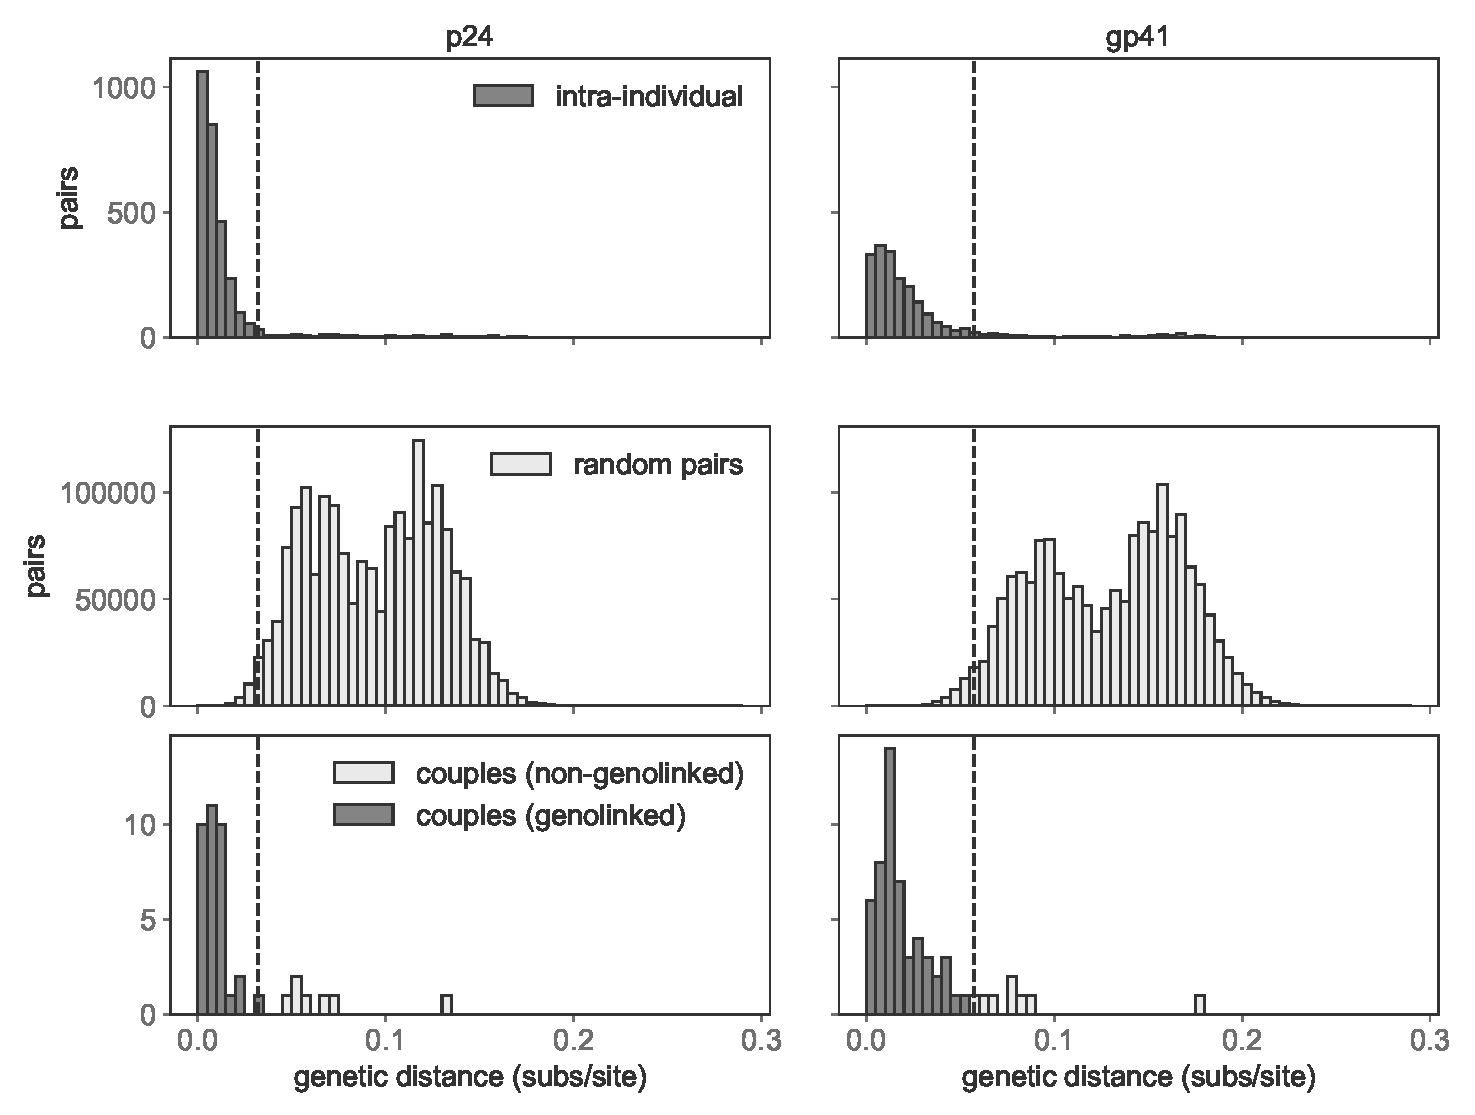
\includegraphics[width=1.0\textwidth]{../figures/eps/genetic_linkage_distr.eps}
    \caption{\protect \textbf{Distribution of pairwise genetic distance in p24 (left) and gp41 (right) among intra-individual pairs (top row), randomly generated index-partner pairs (middle row) and index-partner pairs in monogamous, serodifferent partnerships (bottom row)}. Threshold that jointly maximizes sensitivity and specificity of identifying intra-couple genetic distances (using intra-individual distances as a proxy for ``true positives'' and random pairs as a proxy for ``true negatives'') as identified by Youden's J shown as vertical dotted line.}
    \label{fig:genetic_linkage_distr} % Used for referencing
\end{figure}

\subsubsection*{Phylogenetic topology-based linkage}
In addition to the genetic distance-based linkage described above we also used phylogenetic topology-based linkage to ensure that the evolutionary relationship between sequences from index-partner pairs in the context of other sequences sampled from RCCS participants were evolutionarily consistent with intra-couple transmission. As these results are interpreted alongside the distance-based linkage, we consider only topology and not branch length in our phylogenetic clustering analysis, however, we do collapse any branch lengths $<5\times10^{-4}$ substitutions/site into polytomies to ensure that remaining nodes represent true diversification. The method used to identify phylogenetic topologies consistent with intra-couple transmission is summarized in \textbf{Figure \ref{fig:tree_topo}}. In short, given a phylogenetic tree we first identified all tips in the tree sampled from a given index partner as viral genetic sequences are available for some individuals from multiple time points. We then identified the internal nodes that are immediately parental to monophyletic clades from that index partner (within-index nodes). In the case of singleton tips, the tip itself was considered the within-index node. We then identified the parental nodes of each within-index node (ancestral index nodes) and considered all tips that descend from that node to be putatively linked to the index of interest. This approach therefore accounts for the fact that the common ancestor of genetic diversity sampled from a genuine index-partner pair may not have been directly observed in the index individual due to e.g. lineage turnover between transmission and sampling for viral genetic sequencing. This is particularly important given the fact that viral genomic data is sometimes only available from an RCCS survey visit that occurred well after partner seroconversion. Further, this approach accounts for the fact that a given index partner may have transmitted to multiple RCCS participants or that a seroconverting partner may have also transmitted to other RCCS participants, which would be expected to disrupt non-ambiguous clustering patterns such as nesting of the seroconverting partner's viral genetic diversity within the index partner's viral genetic diversity or the presence of index-partner ``cherries'' (monophyletic clades with only tips from the index or seroconverting partner). Finally, by identifying all within-index nodes in the tree this method accounts for the possibility of superinfection causing an index partner to harbor distinct viral genotypes, provided the genotype transmitted to their partner is sampled. Given the fact that HIV evolution over long time scales is non-linear in nature with large inter-individual variation \citesupp{zanini2015} we do not account for the time of sampling which would require a calibrated model of within-individual viral evolution. \par

To perform phylogenetic topology-based clustering we first identified the set of all available sequences (i.e. from multiple RCCS surveys) from each index and seroconverting partner pair with available viral genetic sequence data covering $>95\%$ of a given region (p24 and gp41). To add additional genetic context from other RCCS participants we also identified the five most closely related sequences (based on Kimura 2-Parameter distance as above), among all available RCCS study participant sequences, to each available sequence from an index or soerconverting partner. The final deduplicated sets of p24 and gp41 sequences including all available sequences for index and seroconverting partner pairs with available sequence data as well as their nearest neighbors were used to infer phylogenetic trees using \textsc{IQ-TREE v.2.2.2.7} \citesupp{minh2020} using \textsc{ModelFinder} \citesupp{kalyaanamoorthy2017} to find the best-fit substitution model with HXB2 as an outgroup. Topology-based clustering was conducted in \textsc{Python v.3.12.4} with \textsc{Baltic v.0.3.0}. Full phylogenetic trees for p24 and gp41 with low-level viremia couples highlighted are shown in \textbf{Figure \ref{fig:full_trees}} and summarized in \textbf{Table \ref{table:linkage}}.


\begin{figure}[!ht] 
    \centering
    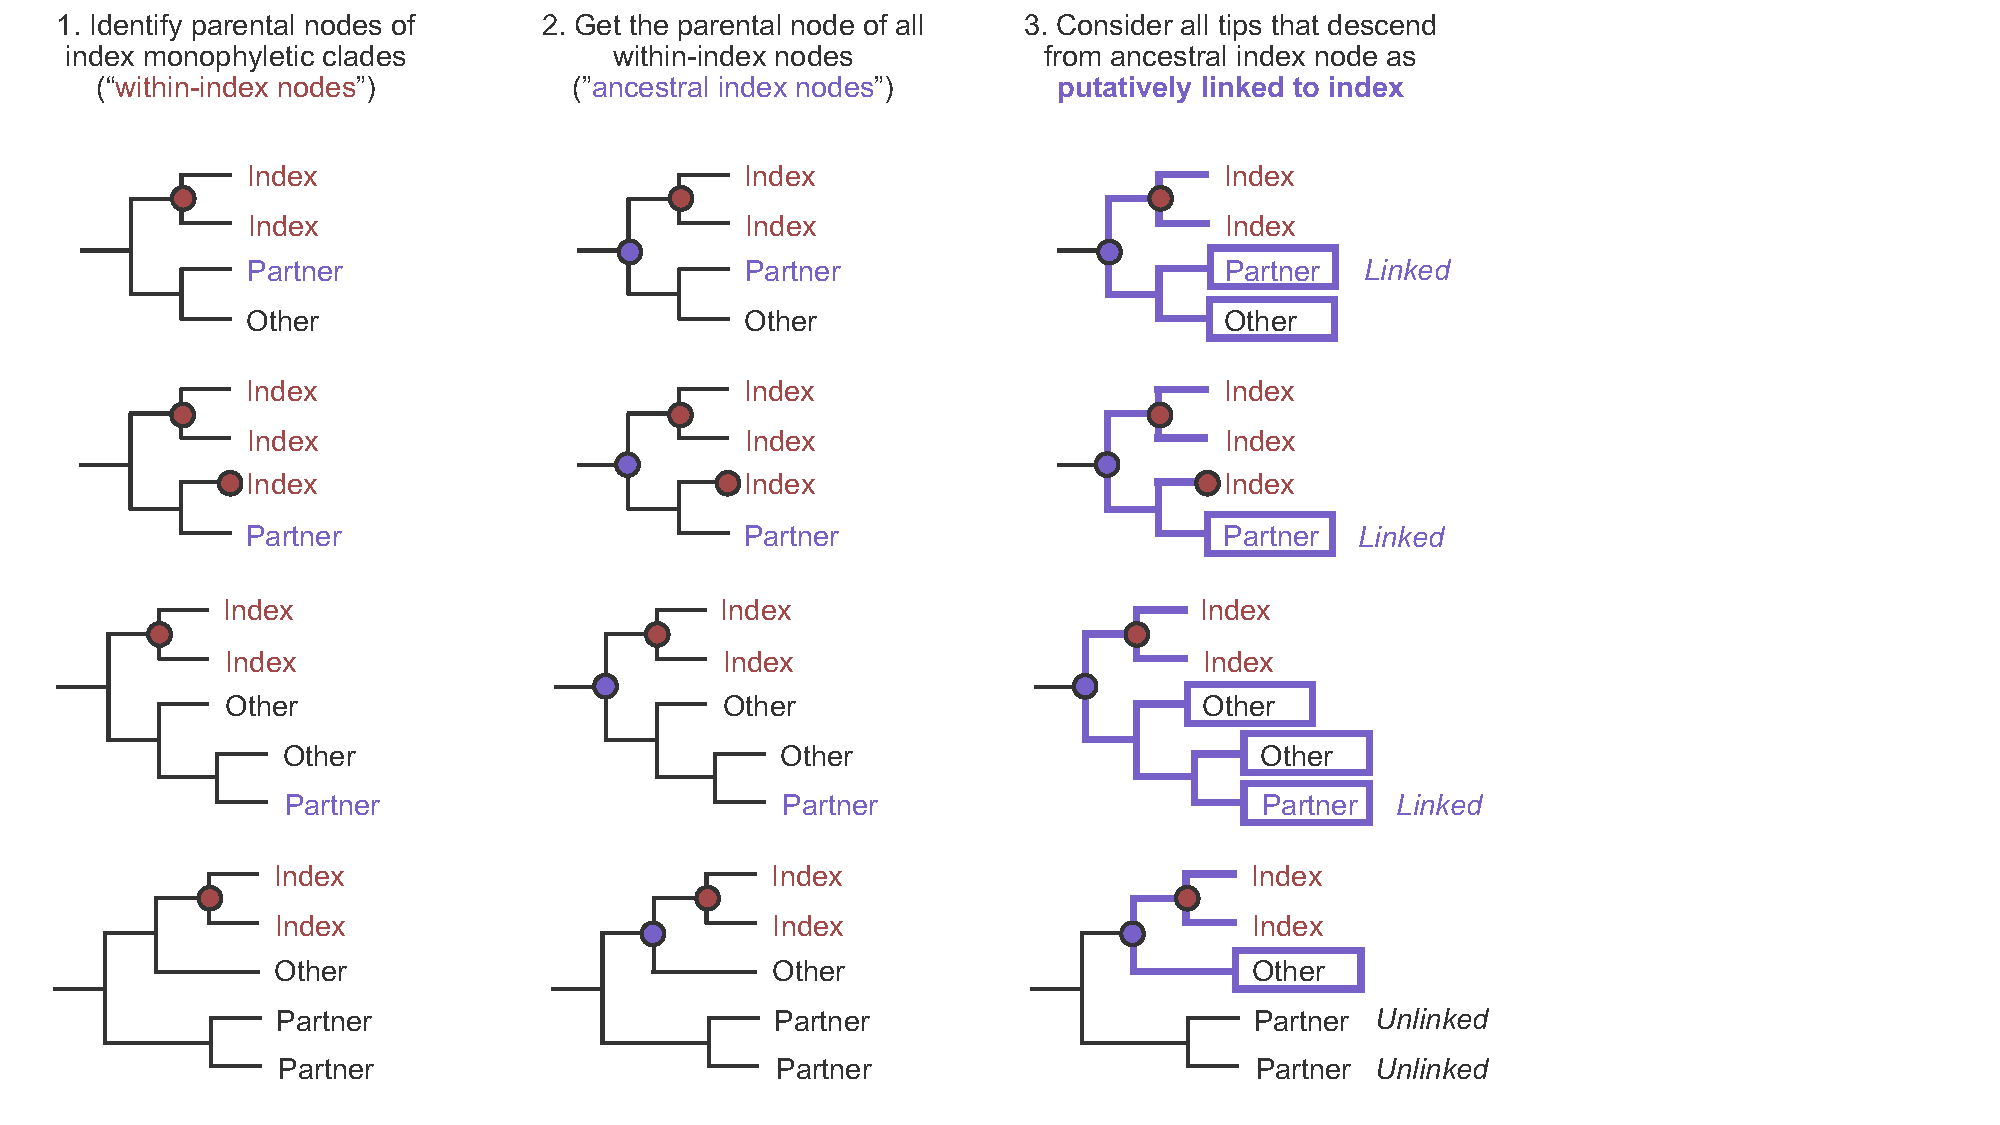
\includegraphics[width=1.0\textwidth]{../figures/pdf/linkage_methods.pdf}
    \caption{\protect \textbf{Method for establishing genetic linkage in transmission pairs using phylogenetic tree topology}.}
    \label{fig:tree_topo} % Used for referencing
\end{figure}

\begin{figure}[!ht] 
    \centering
    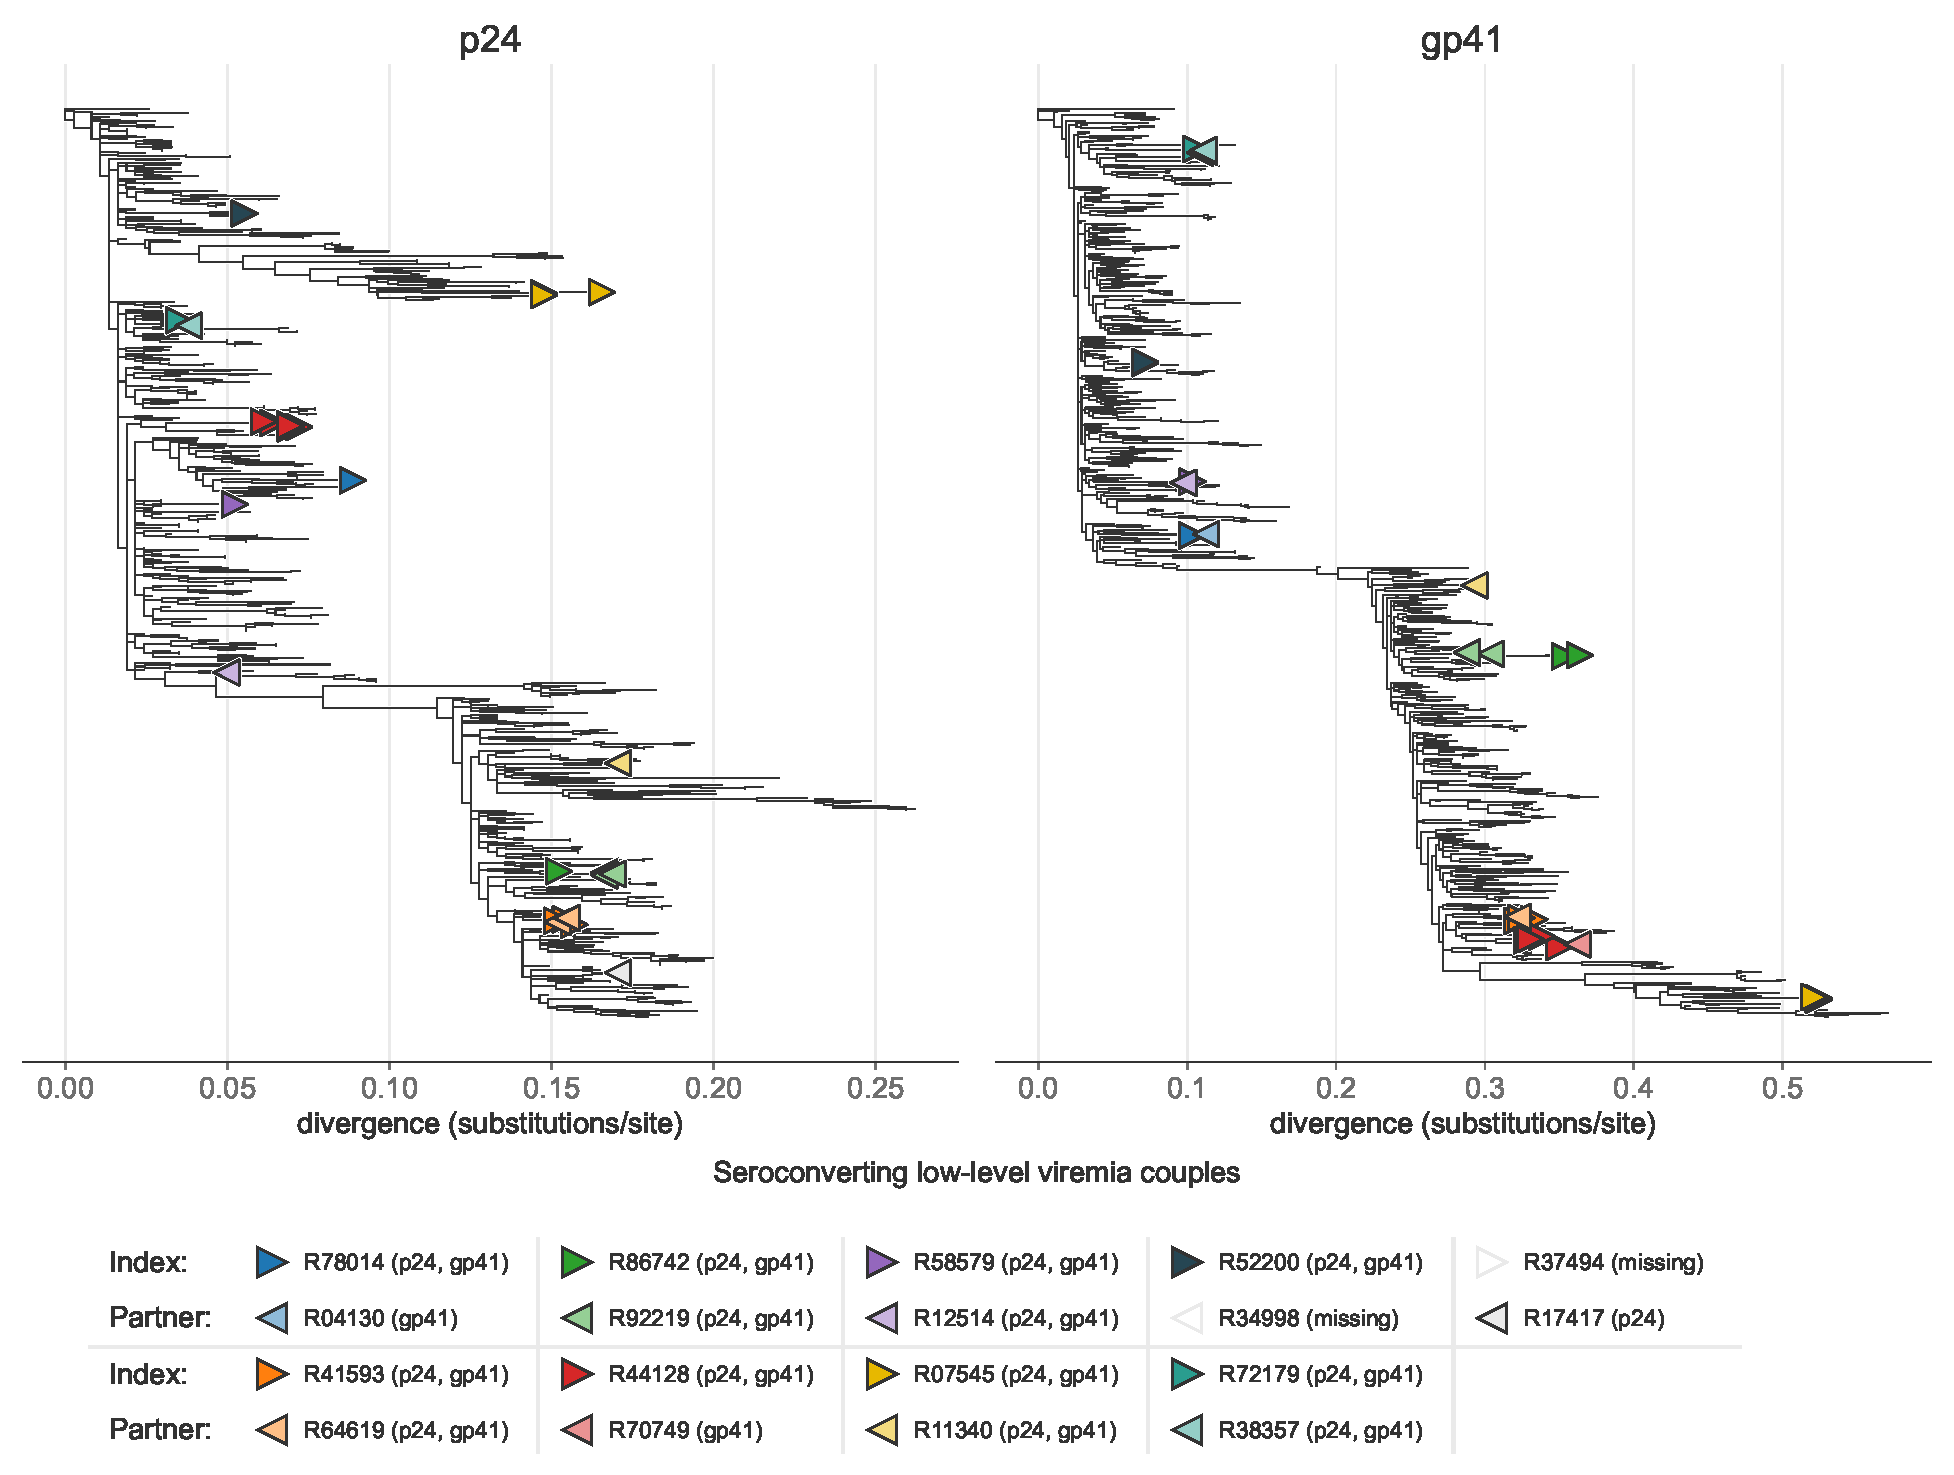
\includegraphics[width=1.0\textwidth]{../figures/eps/full_trees.eps}
    \caption{\protect \textbf{Phylogenetic trees in p24 and gp41 highlighting couples with low-level viremia proximal to first partner HIV seropositivity}. Sequences from initially seropositive index partners shown as right-facing arrows and those from seroconverting partners shown as left-facing arrows. Sequence data is not available for all individuals in both segments. Unlabelled tips are from RCCS study participants, either those in other seroconverting couples or background sequences selected based on genetic distance to individuals in seroconverting couples. Trees are visualized with HXB2 as outgroup. }
    \label{fig:full_trees} % Used for referencing
\end{figure}


\begin{table}[!h]
\caption{\textbf{Genetic linkage among couples in which index partner had low-level viremia proximal to the interval in which partner seroconversion occurred.} For reach sequenced region (p24 and gp41), linkage was determined separately using either genetic distance (``Distance'') or phylogenetic topology (``Tree''). Unavailable linkage data (blank entries) is due to missing viral genomic data for one or both partners in a given region. Lack of genetic linkage implies that direct transmission between the partners is very unlikely, which linkage implies that the genetic sequencing is consistent with direct transmission. Viral loads of the index partner at the sampling times immediately before and after partner seroconversion are shown in \textbf{Table \ref{table:llv}}.}
\begin{tabular}{lccccccc}
\toprule
&\multicolumn{3}{c}{\textbf{p24}}&\multicolumn{3}{c}{\textbf{gp41}}&\\
\cmidrule(lr){2-4}\cmidrule(lr){5-7}&\\
\textbf{Couple}&\textbf{Distance}&\textbf{Tree} & \textbf{Overall} & \textbf{Distance}&\textbf{Tree} & \textbf{Overall} & \textbf{Conclusion} \\
\midrule
R78014$\rightarrow$R04130&&&& ambiguous & linked & likely linked & likely linked\\
R41593$\rightarrow$R64619& linked & linked & linked & linked & linked & linked & linked\\
R86742$\rightarrow$R92219& linked & linked & linked & linked & linked & linked & linked\\
R44128$\rightarrow$R70749&&&&linked&linked&linked&linked\\
R58579$\rightarrow$R12514& unlinked & unlinked & unlinked & linked & linked & linked & linked\\
R07545$\rightarrow$R11340& unlinked & unlinked & unlinked & unlinked & unlinked & unlinked & unlinked\\
R52200$\rightarrow$R34998&&&&&&& NA\\
R72179$\rightarrow$R38357& unlinked & unlinked & unlinked & linked & linked & linked & linked\\
R37494$\rightarrow$R17417&&&&&&& NA\\
\bottomrule
\end{tabular}
\label{table:linkage}
\end{table}

\clearpage

\subsection*{Statistical model relating viral load to transmission rate}

\subsubsection*{Data used in estimating transmission rates}
For each RCCS participant $i$, we summarize their survey data in each of $k=1...19$ survey rounds through the following variables in \textbf{Table \ref{table:rccs_vars}}. From these, we can also calculate several useful transformed data variables for convenience. We additionally define several latent variables that are unobserved but important for inference. 

\begin{table}[hp!]
\centering
\caption{\textbf{Summarized Rakai Community Cohort Study data variables}}
\begin{footnotesize}
\begin{tabular}{p{0.09\columnwidth}L{0.1\columnwidth}p{0.13\columnwidth}p{0.62\columnwidth}}
\toprule
\textbf{Variable}&\textbf{Type}& \textbf{Unit}& \textbf{Description} \\
\midrule
\multicolumn{3}{l}{\textbf{Primary variables}}\\
\midrule
$\text{SEX}_i$ & categorical & 1 & Sex of participant $i$ (Female/Male) \\
%$p_{i,k}$ & binary & 1 & Indicator of whether $i$ participated in survey $k$ (1) or not (0) \\
$c_{i,k}$ & continuous & years (decimal) & Calendar time of participant $i$'s survey interview in survey $k$ \\
$\text{AGE}_{i,k}$ & continuous & years & Age of participant $i$ in survey $k$ \\
$\text{COMM}_{i,k}$ & categorical & 1 & Community type of residence for participant $i$ in survey $k$ (agraria, fishing, trading) \\
$h_{i,k}$ & binary & 1 & Indicator of whether $i$ was HIV seropositive in survey $k$ (1) or not (0) \\
$V_{i,k}$ & continuous & copies/mL & Measured viral load of individual $i$ in survey $k$. Assumed to be 0 when seronegative\\
$v_{i,k}$ & continuous & log$_{10}$ copies/mL & Measured log$_{10}$  viral load of individual $i$ in survey $k$
\\
$\text{ART}_{i,k}$ & binary & 1 & Indicator of whether $i$ self-reports being on HIV antiretroviral therapy at round $k$ or any previous rounds (1) or not (0) (ART-experienced)\\
$m_{i,j,k}$ & binary & 1 & Indicator of whether participant $i$ and participant $j$ report being in a cohabitating partnership in survey $k$ and surveys $k-1$ with $i$ reporting monogamy in both surveys, $j$ being seropositive in survey $k-1$, and $i$ being seronegative in survey $k-1$ (1) or not (0) \\
$s_{i,j,k}$ & binary & 1 & Indicator of seroconversion (1) or not (0) of individual $i$ between survey $k-1$ and $k$, while in a monogomous cohabiting partnership with with individual $j$ \\
\midrule
\multicolumn{3}{l}{\textbf{Transformed variables}}\\
\midrule
$P_i$ & integer vector & 1 & List of survey indices in which individual $i$ participated \\
$t_{i,k}$ & continuous & years (decimal) & Duration between time when $i$ participated in survey round $k-1$ (at time $c_{i,k-1}$) and $k$ (at time $c_{i,k}$) \\
$d_{i,k}$ & categorical & 1 & Epidemiological strata of individual $i$ in survey $k$ as defined by age ($\text{AGE}_{i,k}$), sex ($\text{SEX}_{i,k}$), and community type ($\text{COMM}_{i,k}$) \\
$\text{BD}_{i,k}$ & binary & 1 & Indicator of whether participant $i$ was seropositive and had a viral load below the limit of detection (BD) (limit of detection (LOD) = 40 copies/mL) in survey $k$ (1) or not (0) \\
$\text{MLV}_{i,k}$ & binary & 1 & Indicator of whether participant $i$ had a viral load between the LOD and 200 copies/mL (minimal level of viremia) in survey $k$ (1) or not (0) \\
$\text{LLV}_{i,k}$ & binary & 1 & Indicator of whether participant $i$ had a viral load between 200 and 1,000 copies/mL in survey $k$ (1) or not (0) \\
$\text{VIR}_{i,k}$ & binary & 1 & Indicator of whether participant $i$ had a viral load greater than 1,000 copies/mL (viremic) in survey $k$ (1) or not (0) \\
%\item $b_{i,k}$: Integer, the last RCCS survey prior to $k$ in which $i$ participated; 
$n^{BD}_{i,k}$ & integer & 1 & The number of RCCS surveys from survey 11 and $k$ in which $i$ had a below-detection viral load, $\sum_{x=11}^{k}\text{BD}_{i,x}$ \\
\midrule
\multicolumn{3}{l}{\textbf{Latent variables}}\\
\midrule
$V_{i,k}^*$ & continuous & copies/mL & True viral load of individual $i$ in survey $k$ \\
$v_{i,k}^*$ & continuous & log$_{10}$ copies/mL & True log$_{10}$ viral load of individual $i$ in survey $k$ \\
$\text{FN}_{i,k}$ & binary & 1 & Indicator of whether the viral load measurement from participant $i$ at visit $k$ is a false negative (1) or not (0) \\
$\text{unART}_{i,k}$ & binary & 1 & Indicator of whether participant $i$ was on unreported antiretroviral therapy at any survey since the introduction of antiretroviral therapy (survey 11) prior to survey $k$ (1) or not (0)\\
$\text{init-unART}_{i,k}$ & binary & 1 & Indicator of whether participant $i$ was on unreported antiretroviral therapy for the first time at survey $k$ (1) or not (0) \\
$y_{i,j,k}$ & binary & 1 & Indicator of transmission (1) or not (0) from individual $j$ to individual $i$ between survey $k-1$ and $k$\\
\midrule
\multicolumn{3}{l}{\textbf{Abbreviations}}\\
\midrule
LOD & & & Viral load assay limit of detection, 40 copies/mL  \\
BD & & & A measured viral load value below the limit of detection  \\
FN & & & A false negative viral load measurement   \\
ART & & & Antiretroviral therapy  \\
$\text{init-unART}$  & & & Initiation of unreported antiretroviral therapy \\
unART & & & Unreported antiretroviral therapy \\
\bottomrule
\end{tabular}
\end{footnotesize}
\label{table:rccs_vars}
\end{table}


\newpage

% \subsubsection*{[ASIDE] Transmission model comparison}

% \paragraph*{Form 1 (currently used)}

% Probability of infection in a single sexual act

% \begin{equation}
% P(y=1|V) = 1-\left(1-\rho_{\text{est.}}\right)^{c V}.
% \end{equation}

% Probability of transmission over time, assuming a fraction of sexual acts are conducive to infection

% \begin{equation}
% \begin{split}
% P(y_{i,j,k}=1|t_{i,k},V_{j,k}, m_{i,j,k}=1) & = 1-\left(1-\rho_{\text{prod.}} P(y=1|V)\right)^{f t_{i,k}}\\
% & = 1-\left(1-\rho_{\text{prod.}}\left(1-\left(1-\rho_{\text{est.}}\right)^{c V_{j,k}}\right)\right)^{f t_{i,k}}.
% \end{split}
% \end{equation}

% \begin{itemize}
%     \item $\rho_{\text{prod.}}$ is the fraction of potential infection events that are possible, due to the permissiveness of the sexual encounter
%     \item NOTE: This is actually an approximate formula, because we assume that exactly $f t_{i,k}$ permissive sex acts occur, whereas in reality there is a distribution with this mean
%     \item $V$ and $t$ influence the transmission risk differently
%     \item  $c$, $\rho_{\text{est.}}$ and $\rho_{\text{prod.}}$ all theoretically identifiable
% \end{itemize}


% Another way of thinking about this form: We want a model whereby at each sexual act the probability of transmission is either A) 0 (unproductive act) or is as given by the viral load, $c$ and $\rho_{\text{est.}}$ (in other words a 0 inflated model where each act either has 0\% or 100\% (relative to viral load) productivity. Therefore, we have: $P(y=1 | V) = \rho_\text{prod.}*(1-(1-\rho_\text{est.})^{c V})*1+(1-\rho_\text{prod.})*0 = \rho_{\text{prod.}}\left(1-\left(1-\rho_{\text{est.}}\right)^{c V_{j,k}}\right)$

% \paragraph*{Form 2}

% \begin{equation}
% P(y=1|V) = 1-\left(1-\rho_{\text{est.}}\right)^{c V}.
% \end{equation}

% \begin{equation}
% \begin{split}
% P(y_{i,j,k}=1|t_{i,k},V_{j,k}, m_{i,j,k}=1) & = 1-\left(1-P(y=1|V)\right)^{\rho_{\text{prod.}} f t_{i,k}}\\
% & = 1-\left(1-\rho_{\text{est.}}\right)^{\rho_{\text{prod.}} c V_{j,k}f t_{i,k}}.
% \end{split}
% \end{equation}

% \begin{itemize}
%     \item $\rho_{\text{prod.}}$ is the fraction of sexual encounter that are permissible to infection
%         \item NOTE: This is actually an approximate formula, because we assume that exactly $\rho_{\text{prod.}} f t_{i,k}$ permissive sex acts occur, whereas in reality there is a distribution with this mean
%     \item $V$ and $t$ influence the transmission risk in the exact same way
%     \item  Only $\rho_{\text{est.}}$ and the product of $c$ and $\rho_{\text{prod.}}$ are theoretically identifiable. Either $c$ or $\rho_{\text{prod.}}$ must be fixed for fitting to make sense
% \end{itemize}


% Mike says: Putting $\rho_{\text{prod.}}$ in the exponent is akin to a leaky process whereby a $\rho_{\text{prod.}}$ of 0.5 is like saying every act has a 50\% productivity relative to what would be expected based on $c$, $\rho_{\text{est.}}$, and viral load. Alison: No I don't think so, that's what Form 1 is.  Form 2 is saying that the NUMBER of sex acts if effectively 50\% of what it would have been if 100\% of them were productive


% Mike says : This is not strictly correct if we want the model such that each act has either a 0\% or a 100\% productivity (based on a given viral load). Putting $\rho_{\text{prod.}}$ in the exponent makes $\rho_{\text{prod.}}$ and $c$ non-identifiable and also does not produce an inherently saturating process (i.e. conditional on $c$, $\rho_{\text{est.}}$ and $\rho_{\text{prod.}}$ a higher viral load will always produce a higher transmission rate [Alison: I don't know what this means. The function is still monotonic in $V$, and as $V$ gets larger, it will still tend towards 1]

% \paragraph*{Resolution}

% It seems not to make much intuitive sense why these formulas are different because both ways of thinking about  the process seem equally valid. It turns out, if we fix a mistake that occured in both of them, they actually end up agreeing!

% The mistake is that we assumed the exact number of sex acts occuring in time $t$ is $f t$, wherease in reality this is just the expected number. We can think of sex acts as a Poisson process occuring at rate $f$, and so then the exact number $N$ that occur in an interval is given by Poiss$(N;ft)$. To get the expected transmission probability after a time $t$ we have to sum over each possible number of sex acts $N$ and their probability, multiplied by the transmission probability given $N$ encounters. For either Form 1 or Form 2 of the model, this sum has a closed form solution, and in both cases the transmission risk is the same

% \begin{equation}
% \begin{split}
% P(y_{i,j,k}=1|t_{i,k},V_{j,k}, m_{i,j,k}=1) & = 1-e^{- f t_{i,k} \rho_{\text{prod.}} \left(1-\left(1-\rho_{\text{est.}}\right)^{c V_{j,k}}\right) }.
% \end{split}
% \end{equation}

% Because we know that the transmission rate is relatively low (even at the highest possible viral loads, in a year, the rate of transmission appears to max out around 15\%, we can use the approximation that $e^{-x} \approx 1-x $ when $x \ll 1$ so then


% \begin{equation}
% \begin{split}
% P(y_{i,j,k}=1|t_{i,k},V_{j,k}, m_{i,j,k}=1) & \approx f t_{i,k} \rho_{\text{prod.}} \left(1-\left(1-\rho_{\text{est.}}\right)^{c V_{j,k}}\right).
% \end{split}
% \end{equation}

\subsubsection*{Transmission model}
Our primary interest is in estimating the relationship between index partner viral load and rate of transmission to their seronegative partner. We do this using longitudinal data from pairs of serodifferent individuals in monogamous, cohabitating partnerships. We assume that there is a continuous, increasing relationship between the index partner's viral load ($V$, copies/mL) and the probability per sexual encounter of transmission to their partner. To describe this relationship, we use a simple, yet flexible, mathematical model of stochastic viral establishment.  We assume at each sexual encounter, a number of virions proportional to index partner viral load are ``inoculated'' into the seronegative partner ($c V$), and that each of these virions has an independent probability of establishing infection within this individual ($\rho_{\text{est.}}$). Thus, the \textbf{probability of transmission in a single sexual encounter} ($y=1$) with an individual with viral load $V$ assuming that that sexual encounter is amenable to transmission is

\begin{equation}
P(y=1|V) = 1-\left(1-\rho_{\text{est.}}\right)^{c V}.
\end{equation}

After exactly $N$ sexual encounters occur, the probability of transmission (i.e., the probability that at least one encounter led to successful transmission, $y_N=1$)) is

\begin{equation}
\begin{split}
P(y_N=1|V) & = 1-\left(1-P(y=1|V)\right)^N\\
& = 1-\left(1-\left(1-\left(1-\rho_{\text{est.}}\right)^{c V}\right)\right)^{N}.
\end{split}
\end{equation}

The exact number of sexual encounters it not observable, but we can estimate the average frequency of sexual encounters among monogamous cohabiting couples participating in the RCSS. If we assume that the frequency of sexual encounters per time is $f$ and only a fraction of sexual encounters may be amenable to transmission ($\rho_{\text{prod.}}$), the number of encounters amenable to transmission occurring in a time period $t$ is a thinned Poisson process with rate $\rho_{\text{prod.}} f$, i.e., $N \sim \text{Poiss}(\rho_{\text{prod.}} f t)$. Then, the \textbf{transmission probability over a given duration of follow-up $t_{i,k}$} that individual $i$ is infected by individual $j$ between survey $k-1$ and survey $k$ (indicated by $y_{i,j,k}$=1) is 

\begin{equation}
P(y_{i,j,k}=1|t_{i,k},V_{j,k}, m_{i,j,k}=1) = 1-e^{- f t_{i,k} \rho_{\text{prod.}} \left(1-\left(1-\rho_{\text{est.}}\right)^{c V_{j,k}}\right) }.
\label{eq:prob_intra_trans}
\end{equation}

where $m_{i,j,k}=1$ indicates that $i$ is in a cohabitating relationship with $j$, with $i$ reporting monogamy in surveys $k-1$ and $k$.

Note that we can never directly observe transmission occurring between two individuals. All we can observe is seroconversion of a seronegative partner, but it is always possible that they were infected outside the partnership, and not by the index partner of interest. Therefore, $y_{i,j,k}$ is a latent variable, and the observed data is $s_{i,j,k}$, the seroconversion of individual $i$ between survey $k-1$ and $k$. To incorporate this into the model, we include a rate (per time) of extra-partner transmission, $\beta_\text{extra}$. Then, the overall \textbf{probability of seroconversion over duration of follow-up $t_{i,k}$ due to both between-partner and extra-partner transmission} is

\begin{equation}
P(s_{i,j,k}=1|t_{i,k},V_{j,k}, m_{i,j,k}=1) = 1-e^{-t_{i,k}\left[\beta_\text{extra} + f \rho_{\text{prod.}} \left(1-\left(1-\rho_{\text{est.}}\right)^{c V_{j,k}}\right) \right]}.
\end{equation}


This formula assumes that the viral load of the index partner is known and constant throughout the interval of observation. Due to the nature of data collection in RCCS participants in which participants in a community are interviewed over the course of multiple days, the dates at which the viral load of the index partner were measured may not correspond exactly to the dates at which the serostatus of the initially seronegative partner was determined. Further, we must account for instances where index partner viral load was measured at both survey $k-1$ and survey $k$. Finally, it is possible for an index partner to have their viral load measured, for example, at survey $k-2$ or $k+1$ but not at $k-1$ or $k$. We therefore must first identify the set of survey dates for the index partner that are closest in time to each of the relevant partner HIV testing dates. To do this, we assume that index viral load is piecewise constant and changes in a step-wise fashion at the mid-point between observations, which we call index viral load break-points. When an index viral viral load break-point(s) occurs during the time between their partner's HIV serostatus observations ($c_{i,{k-1}}$, $c_{i,k}$), we discretize the interval into $N^{i,j,k}$ intervals over which the index partner viral load is constant, each with its own duration of time $\tau_{x=1...N^{i,j,k}}^{i,j,k}$. In estimating transmission rate, we include only partnership intervals that fall entirely within two years of index partner viral load observations. Specifically, we ensure $c_{i,k-1}$ and $c_{i,k}$ are no more than two years from an index viral load observations and any viral load break-points within the interval occur no more than two years from the two index viral load observations that define that break-point. Finally, we include only partnership intervals that fall outside of the acute phase of infection for index partners who participated in the RCCS prior to acquiring infection. Specifically, for these index individuals we estimate their date of HIV acquisition as the mid-point between their last HIV- observation and their first HIV+ observation and ensure that $c_{i,{k-1}}$ for all partnership intervals in which they are the index (a given individual can be the index partner in multiple concurrent or asynchronous serodifferent partnerships provided the seronegative individual is monogamous) is greater than 180 days from the estimated seroconversion date. For notation purposes, we introduce an alternative indexing scheme for index partner viral load observations where $V^{i,j,k}_{x}$ indexes the piecewise constant index partner viral loads over the partnership interval defined between survey $k-1$ and $k.$ Validity of a partnership interval based on these two criteria (no more than two years from an index viral load monitoring event, more than 180 days from estimated index partner seroconversion) is indicated by the binary indicator variable $g_{i,j,k}$ where $g_{i,j,k}=1$ indicates a valid partnership interval and $g_{i,j,k}=0$ is invalid. 

Taken together, the \textbf{probability of seroconversion in a given partnership interval} predicted by the model is found by multiplying the probability in each sub-interval defined by a the index partner's most recent viral load measurement: 

\begin{footnotesize}
\begin{equation}
P(s_{i,j,k}=1|\{\tau_{x}^{i,j,k}, V^{i,j,k}_x\}_{x=1}^{N^{i,j,k}},
g_{i,j,k} = 1, m_{i,j,k}=1) = 
1- \prod_{x=1}^{N^{i,j,k}} e^{-\tau_x^{i,j,k}\left[\beta_\text{extra}+f \rho_{\text{prod.}} \left(1-\left(1-\rho_{\text{est.}}\right)^{c V^{i,j,k}_{x}}\right)\right]}.
\end{equation}
\end{footnotesize}

As we only model transmission among valid partnership intervals, as identified by observed initially seronegative partner monogamy ($m_{i,j,k} = 1$) and observed time from index partner seroconversion ($g_{i,j,k}=1$), we fix the likelihood of valid partnership intervals at 1 regardless of whether seroconversion is observed ($s_{i,j,k}=1$) or not ($s_{i,j,k}=0$). 
\begin{align}
P(s_{i,j,k}|m_{i,j,k}=0) &= 1 \\
P(s_{i,j,k}|g_{i,j,k}=0) &= 1 \\
\end{align}

A summary of the model parameters and their use in the estimation procedure is provided in \textbf{Table \ref{table:trans_params}}. Details on the inference procedure we use to estimate the model parameters most consistent with the data is provided in a later section. 


\begin{table}[h!]
\centering
\caption{\textbf{Transmission model parameters}}
\begin{tabular}{p{0.1\textwidth}p{0.4\textwidth}p{0.08\textwidth}L{0.35\textwidth}}
\toprule
\textbf{Parameter} & \textbf{Description} & \textbf{Unit} & \textbf{Value}\\
\midrule
$f$ & Number of sexual acts per year & year$^{-1}$ & Fixed, 108/year \cite{gray2001} \\
$c$ & Constant of proportionality relating blood viral load to infectious dose during heterosexual sex & mL & Fixed, $c=1$ \\
$\rho_\text{est.}$ & Probability of a single virion establishing infection in a seronegative person given transmission & 1 & Estimated,\newline Prior: $\text{logit}(\rho_\text{est.}) \sim$ Normal($\mu=0$,$\sigma=5$)\\
$\rho_\text{prod.}$ & Fraction of heterosexual acts that are amenable to transmission & 1 &  Estimated, \newline Prior: $\text{logit}(\rho_\text{prod.}) \sim \text{Half-Normal}(\mu=0,\sigma=5)$ \\
$\beta_\text{extra}$ & Extra-partner transmission rate & year$^{-1}$  &  Estimated,  \newline Prior: Informed by sequencing data; see \textbf{Parameter Inference} section\\
\bottomrule
\end{tabular}
\label{table:trans_params}
\end{table}
\clearpage

\subsubsection*{Observational model of participant viral loads}

The transmission model described above assumes that transmission rate is a continuous increasing function of index partner viral load. However, the true viral load of RCCS participants cannot be directly observed and must be measured with a viral load assay. These assays have inherent limits of detection and return either a ``below-detection" reading or a continuous viral load measurement. To account for this discretization of continuous viral load we implemented an imputation procedure to estimate the true viral load in the case of below-detection readings. 

Further, upon visually inspecting longitudinal viral load values from RCCS participants with no reported antiretroviral therapy (ART) use, we noticed occasional undetectable viral loads along with much higher values that were in the expected range of pre-treatment set-point viral loads. The overall distribution of viral load values in these individuals followed an approximately log-normal distribution (consistent with many prior studies of the distribution of viral load set-points \cite{fraser2007, blanquart2016}), with a clear an unexpected spike at values below detection values (\textbf{Figure \ref{fig:pre_treatment_copies}}). Further, the proportion of measurements below the detection limit increased from 8\% among measurements taken in RCCS survey rounds 1 through 10 (\var{r1_minYear} through \var{r10_maxYear}) prior to the widespread availability of ART in this setting, to 18\% among measurements taken in rounds 11 through 19 (\var{r11_minYear} through \var{r19_maxYear}) which spans the Universal Test and Treat era. Together, these observations suggest that some undetectable viral load values in individuals reporting no current or prior ART use may be false negatives due to assay failure or are due to unreported ART use. We believed that either excluding these below detection values or taking them as true measurements of undetectable viremia could bias estimates of the transmission rate inferred at low viral loads. 

Consequently, we utilized a mixture-model-based probabilistic framework to identify the pre-treatment below detection limit values most likely to be false negatives, and then impute estimated true values based on the estimated intra-individual viral load distributions. Given the very high rates of viral load suppression among treatment-experienced people with HIV in this setting ($>95\%$ \cite{martin2026}, \textbf{Figure \ref{fig:treatment_copies}}), we assume that all below-detection viral loads from individuals self-reporting ART use are truly below the limit of detection (LOD) (i.e., true negatives). Similarly, among individuals who we infer to be on unreported treatment, we assume that all below-detection observations are truly below the LOD. Consequently, we only impute below-detection viral loads to be above the LOD when individuals are not on reported and not expected to be on unreported treatment. 


\begin{figure}[htbp] % h! forces the figure to stay "here"
    \centering
    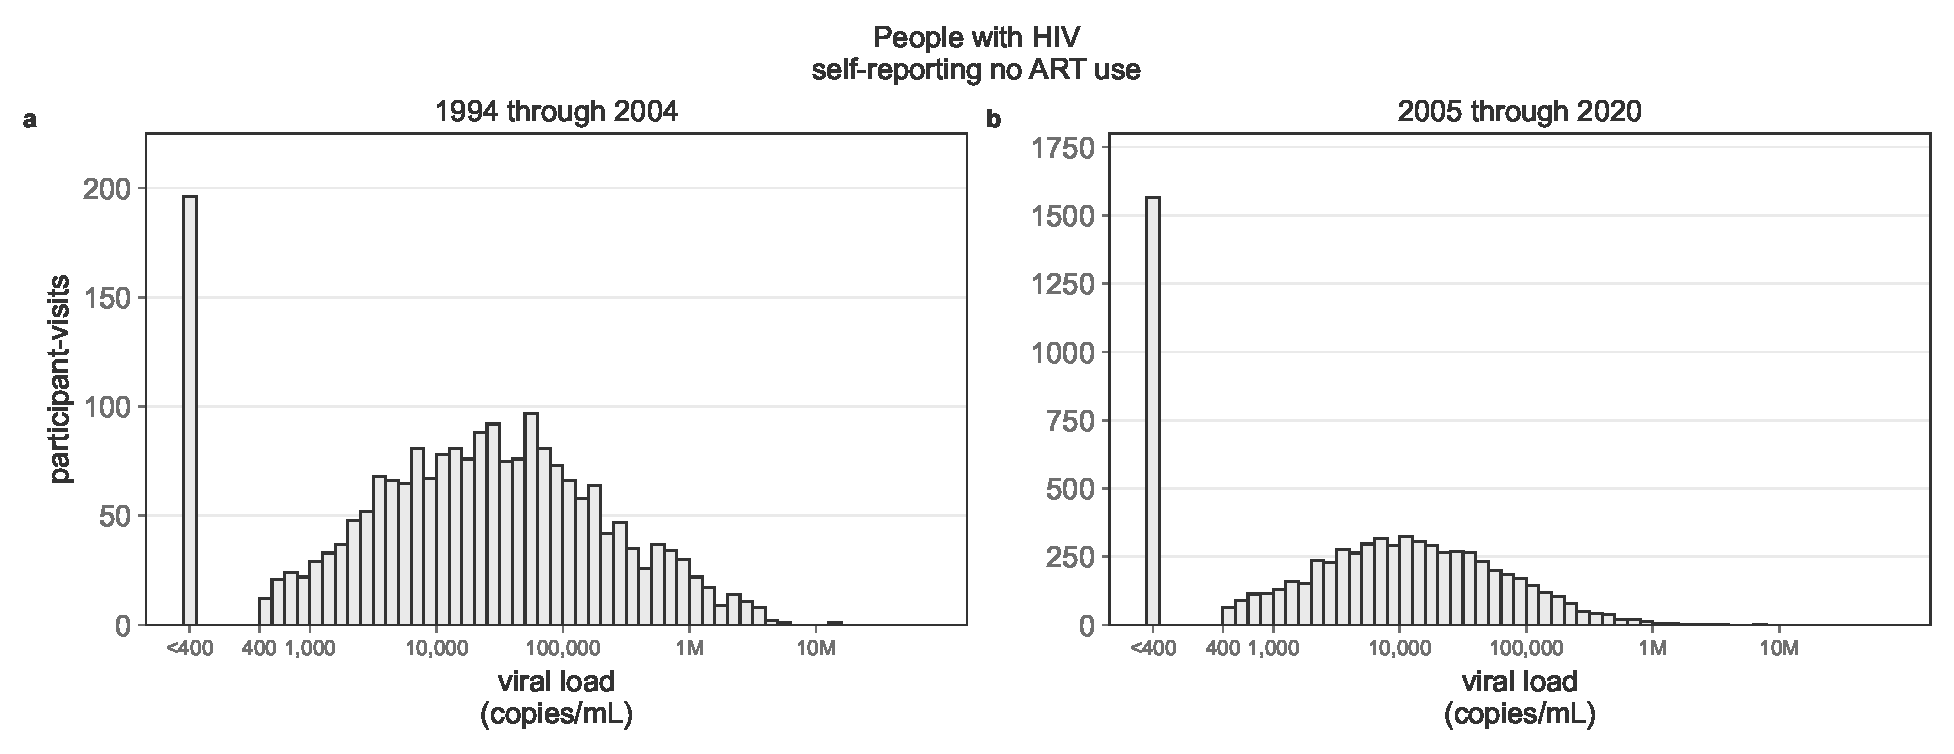
\includegraphics[width=1.0\textwidth]{../figures/eps/pre_treatment_copies.eps}
    \caption{\protect \textbf{Viral load of participants in the Rakai Community Cohort Study (RCCS), \var{r1_minDate}-\var{r19_maxDate} self-reporting no use of antiretroviral therapy.} Stratified by RCCS survey, i.e. survey 1 through 10 (A) v. survey 11 through 19 (B). BD indicates below the assay limit of detection. 
    }
    \label{fig:pre_treatment_copies} % Used for referencing
\end{figure}

\begin{figure}[htbp] % h! forces the figure to stay "here"
    \centering
    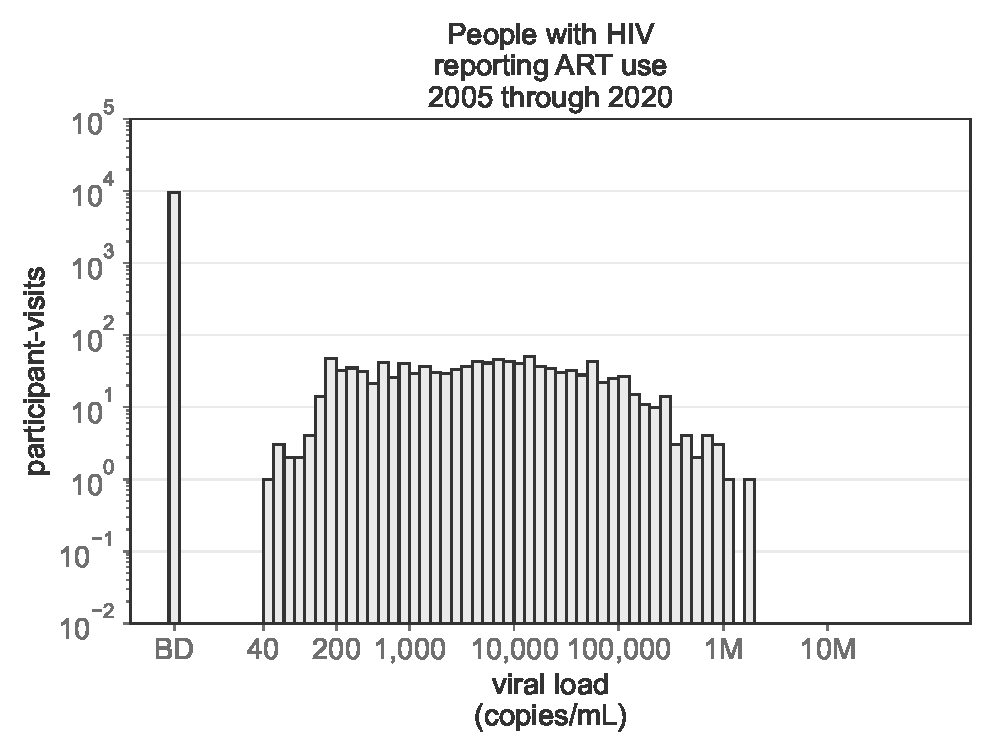
\includegraphics[width=0.5\textwidth]{../figures/eps/treatment_copies.eps}
    \caption{\protect \textbf{Viral load of participants in the Rakai Community Cohort Study (RCCS), \var{r1_minDate}-\var{r19_maxDate} self-reporting use of antiretroviral therapy.} All participants prior to 2005 presumed to be treatment-naive. BD indicates below the assay limit of detection. Note that the y axis on a log scale. 
    }
    \label{fig:treatment_copies} % Used for referencing
\end{figure}



To probabilistically impute putative false-negative values among untreated individuals, we must first calculate the probability that any given below-detection value is truly a false negative and not the result of expected variability in viral loads. This requires a model of pre-treatment viral load variability between individuals in the population and within an individual over time. We assume that untreated individuals included in our analysis (which restricts to those expected to be $>180$ days from seroconversion) are at an approximate set-point viral load, and that individual observed viral loads may vary around this value over time. At the population-level, $\log_{10}$ set-point viral loads are assumed to be normally distributed (mean$=\mu_0 $, standard deviation (s.d.)$=\Omega_\mu $), and at the individual level, $\log_{10}$ viral load variation around set-point is also assumed to be normally distributed (population-mean variability$=\sigma_0$, s.d.$=\Omega_\sigma $). Formally, this is a mixed-effects model where the \textbf{\textit{true}} \textbf{viral load of an untreated individual} $i$ at survey $k$  (denoted $v_{i,k}^*$), defined by the absence of both reported ART use ($\text{ART}_{i,k}$ and unreported (latent) ART use ($\text{unART}_{i,k}$), is assumed to follow the distribution
\begin{align}
(v_{i,k}^*|\text{ART}_{i,k}=0,\text{unART}_{i,k}=0) & \sim \text{Normal}(\mu=\mu_i, \sigma=\sigma_i)
\label{eq:spvl}
\end{align}

with individual parameters being a combination of fixed (population) effects and individual (random) effects:
\begin{equation}
\begin{split}
\mu_i &= \mu_0 + \Omega_\mu\eta_{\mu,i} \\
\sigma_i &= \sigma_0e^{\Omega_\sigma\eta_{\sigma,i}}\\
\eta_{\mu,i} & \sim \text{Normal}(\mu=0,\sigma=1)\\
\eta_{\sigma,i} & \sim \text{Normal}(\mu=0,\sigma=1).
\end{split}
\end{equation}
Unreported use of ART complicates our interpretation of viral loads. As mentioned above, based on the increased proportion of below-detection viral loads among those self-reporting not to be on treatment after the introduction of ART, we suspect that some of these individuals are actually on ART. Based on the observed viral load distribution of individuals self-reporting current or past ART use (\textbf{Figure \ref{fig:treatment_copies}}), we assume that the distribution of viral loads among individuals who are currently or have ever been on unreported ART follows a mixture model with one component for values below the limit of detection (i.e., ART is currently taken and suppressive) and another for detectable values (i.e. due to lapses in adherence or the emergence of resistance). We assume that viral load values below the limit of detection due to ART use are uniformly distributed between 0 and the LOD (on the copies/mL scale) (which we refer to as $\text{Distr}(v^*|\text{ART-TN})$),
\begin{align}
\text{Distr}(v^*|\text{ART-TN}) &= (v^*|\text{ART-TN}) = \text{log}_{10}\text{Uniform}(0,\text{LOD}) \\
\text{Distr}(V^*|\text{ART-TN}) &= (V^*|\text{ART-TN}) = \text{Uniform}(0,\text{LOD}),
\label{eq:distr_art_bd}
\end{align}

and we test the sensitivity of our inferences to this assumption using sensitivity analyses.  Viral loads that are above the LOD among individuals with unreported ART use are assumed to be follow a log-Normal distribution with mean $\mu_\text{unART}$ and standard deviation $\sigma_\text{unART})$. The mixing parameter, $\theta$, dictates the probability of a suppressed viral load (below the LOD) among individuals who self-report no ART use but have some past or present unreported ART use. Therefore, the \textbf{\textit{true }}\textbf{viral load of an individual} $i$ \textbf{with past or current unreported treatment use} at survey $k$ is assumed to follow the distribution
\begin{align}
\begin{split}
(v_{i,k}^*|\text{ART}_{i,k}=0,\text{unART}_{i,k}=1) & \sim \theta\text{Distr}(v^*|\text{ART-TN})\\
&\quad +(1-\theta)\text{Normal}_{\text{log}_{10}\text{LOD}}^{\infty}(\mu=\mu_\text{unART}, \sigma=\sigma_\text{unART}),
\label{eq:spvl_unart}
\end{split}
\end{align}
where Normal$_a^b$ represents a normal distribution left-truncated at $a$ and right-truncated at $b$.

However, to calculate the likelihood of model parameters given observed viral loads, we need to account for three factors that obscure observed values relative to true ones: 1) Viral load assays have limits of detection, and viral loads are reported as either below-detection (BD) or a numeric value greater than the LOD, 2) We suspect that viral load assays (or the sample preparation steps before them) produce false negative readings (FNs) that spuriously produce BD observations regardless of the true viral load, and 3) Unreported ART use is not observed and we do not know which individuals who report no ART use are actually on unreported treatment. 

We first adjust the generative models above to account for the assay limits of detection. To do this, we integrate the intra-individual viral load distributions up to the LOD to calculate the total probability of observing a BD value, not yet accounting for the potential for false negatives. 
\textbf{For individuals with no ART use, the probability of a true negative (below detection limit) viral load value is}

\begin{equation}
P(\text{BD}_{i,k} | \text{ART}_{i,k} = 0, \text{unART}_{i,k} = 0, \text{FN}_{i,k}=0) = \int_{-\infty}^\text{LOD}\text{Normal}(x | \mu=\mu_i, \sigma=\sigma_i)dx 
\end{equation}
where $\text{Normal}(x | \mu, \sigma)$ evaluates the likelihood of a Normal distribution with mean $\mu$ and standard deviation $\sigma$ at a value of $x$. We note that $\int_{-\infty}^\text{LOD}\text{Distr}(v^*|\text{BD}) = 1$ by definition. 

\textbf{For individuals with unreported ART use, the probability of true negative (below detection limit) viral load value is}
\begin{equation}
P(\text{BD}_{i,k} | \text{ART}_{i,k} = 0, \text{unART}_{i,k} = 1) = \theta 
\end{equation}

Therefore, the \textbf{likelihood (probability of observation given model parameters) of a viral load value for an untreated individual, assuming the observation is not a false negative} ($\text{FN}_{i,k} = 0$) is given by
\begin{equation}
\footnotesize
P(v_{i,k}|\text{ART}_{i,k}=0,\text{unART}_{i,k}=0, \text{FN}_{i,k}=0) = \begin{cases} 
    \text{Normal}(v_{i,k} | \mu=\mu_i, \sigma=\sigma_i) & \text{if } v_{i,k} >\text{ LOD} \\
     \int_{-\infty}^\text{LOD}\text{Normal}(x | \mu=\mu_i, \sigma=\sigma_i)dx  & \text{if } v_{i,k} = \text{ BD}.
\end{cases}
\label{eq:pt_intra_indiv_vl}
\end{equation}

Similarly, the \textbf{likelihood of a viral load value for an individual on current or past unreported ART} is given by
\begin{equation}
\footnotesize
P(v_{i,k}|\text{ART}_{i,k}=0,\text{unART}_{i,k}=1) = \begin{cases} 
    \text{Normal}(v_{i,k} | \mu=\mu_\text{unART}, \sigma=\sigma_\text{unART}) & \text{if } v_{i,k} >\text{ LOD} \\
     \theta & \text{if } v_{i,k} =\text{ BD}.
\end{cases}
\label{eq:unart_intra_indiv_vl}
\end{equation}

As described above, we also need to account for the fact that false negative observations can further confound observed viral load values among individuals who are not ART. We model assay false negatives as an all-or-nothing process: they either result in a below-detection observation regardless of the true value or have no effect on observed viral loads. That is, 

\begin{equation}
P(v_{i,k}|\text{FN}_{i,k}=1) = \begin{cases} 
    0 & \text{if } v_{i,k} >\text{ LOD} \\
    1 & \text{if } v_{i,k} \leq\text{ LOD}. \\
\end{cases}
\label{eq:fn_vl}
\end{equation}

Therefore, the probability distribution of observed viral load values is assumed to follow a mixture model between the expected distribution given that the observation is not a false negative (\textbf{Eqs. \ref{eq:pt_intra_indiv_vl}}) and the expected distribution given that the observation is a false negative (\textbf{Eqs. \ref{eq:fn_vl}}). The mixing parameter is the probability that any given measured viral load is a false negative ($P(\text{FN}_{i,k}=1) = \pi$). The \textbf{likelihood of a viral load conditional on not being on treatment} is thus 
\begin{align}
\footnotesize
\begin{split}
P(v_{i,k}|\text{ART}_{i,k}=0,\text{unART}_{i,k}=0) &= (1-\pi)P(v_{i,k}|\text{ART}_{i,k}=0,\text{unART}_{i,k}=0, \text{FN}_{i,k}=0) \\
    &\qquad + \pi P(v_{i,k}|\text{FN}_{i,k}=1) \\
    & = \begin{cases}
        (1-\pi) \text{Normal}(v_{i,k} | \mu=\mu_i, \sigma=\sigma_i)  & \text{if } v_{i,k} >\text{ LOD} \\
        (1-\pi) \int_{-\infty}^\text{LOD}\text{Normal}(x | \mu=\mu_i, \sigma=\sigma_i)dx + \pi  & \text{if } v_{i,k} =\text{ BD}. \\
    \end{cases}
\end{split}
\end{align}

Additionally, we must account for the fact that unreported treatment status (unART) is not observed. To do so, we again turn to a mixture-model formulation in which the probability of a given viral load measurement among individuals self-reporting no current or past treatment is a mixture of one component given that that individual is truly pre-treatment (that is, no current or prior unreported treatment use) and another given that that individual is on current or past unreported treatment. Considering the fact that this subset of RCCS participants all self-report not being on treatment, we assume they do not initiate ART in the absence of strong evidence to the contrary in the form of below-detection viral loads.
%This approach assumes that individuals do not initiate unreported ART prior to their first observed below-detection observation and that all observed viral load variation up to that point is attributable to intra-individual pre-treatment variability. Concordantly, this implies that an individual will have a below-detection viral load at the first RCCS survey at which they are on unreported ART.
To model this process we define an additional parameter, $\gamma_k$, that defines the probability that an individual not on unreported ART at round $k-1$ initiates levels of ART sufficient to reduce viral loads below the LOD by round $k$, indicated by $\text{init-unART}_{i,k}$.  Formally, this means that
\begin{equation}
P(v_{i,k}|\text{ART}_{i,k}=0, \text{init-unART}_{i,k}=1) = \begin{cases}
    0 &\text{if } v_{i,k} > \text{LOD} \\
    1 &\text{if } v_{i,k} = \text{BD}.
\end{cases}
\end{equation}

Given the lack of treatment availability prior to survey round 11, we fix $\gamma_k$ at 0 when $k \leq 10$,
\begin{equation}
\gamma_k = 
\begin{cases}
0 & \text{if } k \leq 10 \\
\gamma & \text{if } k > 10.
\end{cases}
\end{equation}

This approach assumes that individuals do not initiate unreported ART prior to their first observed below-detection observation and that all observed viral load variation up to that point is attributable to intra-individual pre-treatment variability. Concordantly, this implies that an individual will have a below-detection viral load at the first RCCS survey at which they are on unreported ART.

Following the introduction of this new parameter we update our viral load likelihoods slightly for individuals not on reported treatment, 

\begin{equation}
\begin{split}
P(v_{i,k} | \text{ART}_{i,k}=0, \text{unART}_{i,k}=0, \text{init-unART}_{i,k}=0) = \\
\begin{cases}
        (1-\pi) \text{Normal}(v_{i,k} | \mu=\mu_i, \sigma=\sigma_i)  & \text{if } v_{i,k} >\text{ LOD} \\
        (1-\pi) \int_{-\infty}^\text{LOD}\text{Normal}(x | \mu=\mu_i, \sigma=\sigma_i)dx + \pi  & \text{if } v_{i,k} =\text{ BD}, \\
    \end{cases}
\end{split}
\end{equation}

and for individuals on unreported treatment prior to round $k$,
\begin{equation}\begin{split}
P(v_{i,k} | \text{ART}_{i,k}=0, \text{unART}_{i,k}=1, \text{init-unART}_{i,k}=0) = \\
\begin{cases}
        \text{Normal}(v_{i,k} | \mu=\mu_\text{unART}, \sigma=\sigma_\text{unART})  & \text{if } v_{i,k} >\text{ LOD} \\
        \theta  & \text{if } v_{i,k} =\text{ BD}, \\
    \end{cases}
\end{split}
\end{equation}

As a result, there are three mechanisms that can produce a below-detection observation in round $k$ among someone not on unreported or reported ART in round $k-1$: 1) a false negative, which occurs with probability $\pi$, 2) a true negative, which occurs with probability $P(\text{BD}_{i,k} | \text{ART}_{i,k} = 0, \text{unART}_{i,k} = 0, \text{FN}_{i,k}=0) = \int_{-\infty}^\text{LOD}\text{Normal}(x | \mu=\mu_i, \sigma=\sigma_i)dx$, which we refer to as $P(\text{TN}_{i,k}|\text{noART})$ as shorthand and 3) (unreported) treatment initiation which occurs with probability $\gamma_k$. Therefore, the probability that any given below-detection is indicative of ART initiation is given by

\begin{equation}
\begin{split}
P(\text{init-unART}_{i,k}=1|\text{ART}_{i,k}=0,\text{unART}_{i,k-1}=0, \text{BD}_{i,k}=1) = \\
\frac{\gamma_k}{\gamma_k + (1-\gamma_k)\pi + (1-\gamma_k)(1-\pi)P(\text{TN}_{i,k}|\text{noART})}
\end{split}
\end{equation}
where we include the $(1-\gamma_k)$ and $(1-\pi)$ terms in the denominator to account for the fact that treatment initiation precludes the other two mechanisms and the fact that a false negative may occur even if the true value is a true negative. We therefore can calculate the probability that an individual has ever been on unreported treatment prior to, but not including, round $k$ as a function of the probability that any single below-detection observation since ART was made available was not due to treatment initiation, raised to the power of the number of below-detection observations between the beginning of ART availability and round $k$. Specifically, \textbf{the likelihood of unreported ART use prior to round $k$} becomes

\begin{equation}
\Gamma_{i,k} = \begin{cases}
    0 & \text{if } k \leq 11 \\
    1 - \left(1 - P(\text{init-unART}_{i,k}=1|\text{ART}_{i,k}=0,\text{unART}_{i,k-1}=0, \text{BD}_{i,k}=1\right)^{n_{i,k-1}^\text{BD}} & \text{if } k > 11.
\end{cases}
\end{equation}
With this, we can construct the complete \textbf{viral load likelihood among individual self reporting no treatment}, which sums over the possible states of: 1) no past or current unreported ART use which occurs with probability $(1-\Gamma_{i,k})(1-\gamma_k)$, 2) recent initiation of unreported ART with no past initiation which occurs with probability $(1-\Gamma_{i,k})\gamma_k$, and 3) past and potentially current unreported ART which occurs with probability $\Gamma_{i,k}$, as
\begin{equation}
\begin{split}
P(v_{i,k}|\text{ART}_{i,k}=0) &= (1-\Gamma_{i,k})(1-\gamma_k) P(v_{i,k}|\text{ART}_{i,k}=0,\text{unART}_{i,k}=0, \text{init-ART}_{i,k}=0) \\
&\qquad +(1-\Gamma_{i,k})\gamma_kP(v_{i,k}|\text{ART}_{i,k}=0,\text{unART}_{i,k}=0, \text{init-ART}_{i,k}=1) \\
&\qquad +\Gamma_{i,k}P(v_{i,k}|\text{ART}_{i,k}=0, \text{unART}_{i,k}=1). \\
\end{split}
\end{equation}
%We model the probability that individual $i$ was on unreported treatment prior to at or round $k$ as a function of all observed viral load values up to and including at survey $k$, the intra-individual viral load distribution assuming no unreported ART use (\textbf{Eq. \ref{eq:pt_intra_indiv_vl}}), and the intra-individual viral load distribution assuming unreported ART use (\textbf{Eq. \ref{eq:unart_intra_indiv_vl}}). Specifically, we first calculate the probability that any observed viral load arose from the distribution assuming no unreported ART use under the assumption that all viral loads from individuals self-reporting no treatment arise from either the intra-individual viral load distribution given no unreported treatment use (\textbf{Eq. \ref{eq:pt_intra_indiv_vl}}) or the intra-individual viral load distribution given unreported treatment (\ref{eq:unart_intra_indiv_vl}), 
%\begin{equation}
%P(\text{unART}_{i,k} = 1|\text{ART}_{i,k}=0, v_{i,k}) = \begin{cases} 
%    0 & \text{if } k \leq 10  \\
%     \frac{P(v_{i,k}|\text{ART}_{i,k}=0,\text{unART}_{i,k}=1)}{P(v_{i,k}|\text{ART}_{i,k}=0)} & \text{if } k > 10,
%\end{cases}
%\end{equation}
%where ART was assumed to be unavailable through survey round 10. 

%Then, we can calculate the probability of having been on unreported ART at that round or at any previous rounds, based on all previously observed viral loads,

%\begin{equation}
%\Gamma_{i,k} = 1 - \prod_{x=1:P_{i,x}=1}^{k}\left( 1 - %P(\text{unART}_{i,k} = 1|\text{ART}_{i,k}=0, v_{i,k})\right),
%\end{equation}
%where $x=1:P_{i,x}=1$ indexes over all surveys in which participant $i$ participated ($P_{i,x}=1$).
%Because we are only attempting to impute putative false-negative observations among viral loads taken from individuals self-reporting no treatment, we do not explicitly model the probability distribution of observed viral loads among individuals self-reporting treatment. Formally, this can be expressed as: 
%\begin{equation}
%P(v_{i,k} | \text{ART}_{i,k}=1) = 1.
%\end{equation}

Finally, with the parameters of the probability distributions above we can \textbf{probabilistically impute the true values of below detection limit viral load measurements} for each individual at each survey round for use in our \textbf{transmission model}. Imputed viral load values are treated as free parameters to be estimated in the model. 

We define $\tilde{V}_{i,k}$ as the imputed viral load (on the copies/mL scale) for individual $i$ at survey $k$. As we assume that all below-detection observations among those self-reporting treatment are ``true negatives'', among individuals self-reporting ART use we either use the observed viral load if above the LOD or impute the true value according to $\text{Distr}(V^*|\text{ART-TN})$,
\begin{align}
(\tilde{V}_{i,k}|\text{ART}_{i,k}=1) = \begin{cases} 
    V_{i,k} & \text{if } V_{i,k} > \text{LOD} \\
    \sim\text{Distr}(V^*|\text{ART-TN}) & \text{if } v_{i,k} \leq \text{LOD}. \\
\end{cases}
\end{align}

Among individuals self-reporting no ART use, we also use the observed viral if it is above the LOD,
\begin{align}
(\tilde{V}_{i,k}|\text{ART}_{i,k}=0) = \begin{cases} 
    V_{i,k} & \text{if } V_{i,k} > \text{LOD}. \\
\end{cases}
\end{align}
Following \textbf{Eq. \ref{eq:prob_intra_trans}}, for the above two cases, the imputed viral loads can then be used directly to calculate the probability of intra-couple transmission from individual $j$ to individual $i$ (note that as above $j$ is the potentially transmitting index partner) over time $t_{i,k}$ given observed index viral load $V_{j,k}$ and cohabitating monogamy $m_{i,j,k}=1$ as

\begin{equation}
    P\left(y_{i,j,k}=1|t_{i,k},V_{j,k},m_{i,j,k}=1, (\text{ART}_{j,k}=1 |V_{j,k}>\text{LOD})\right) = 1 - e^{-ft_{i,k}\rho_\text{prod.}(1-(1-\rho_\text{est.})^{c\tilde{V}_{j,k}}}.
\end{equation}

Among individuals self-reporting no ART use with below-detection viral loads, we impute potential values of the true viral load under each of the following three cases: 
\begin{enumerate}
\item $V_{i,k}$ is a false negative (i.e. the true viral load $V^*_{i,k}$ is not necessarily below the LOD) and $i$ is not on unreported ART by survey $k$, in which case the viral load follows the intra-individual pre-treatment viral load distribution (\textbf{Eq \ref{eq:pt_intra_indiv_vl}}). For notation simplicity we use noART-FN as shorthand for $(\text{ART}_{i,k}=0,\text{unART}_{i,k}=0,\text{init-unART}_{i,k}=0,\text{FN}_{i,k}=1)$. The probability of this event occurring is the product of the probability not having initiated unreported treatment prior to round $k$, not having initiated unreported treatment at round $k$, and of having a false negative. Formally,
\begin{align}
P(\text{noART-FN})_{i,k} &= (1-\Gamma_{i,k})(1-\gamma_k)\pi \\
(\tilde{V}_{i,k}|\text{noART-FN}) &= \begin{cases} 
    \sim 10^{\text{Normal}(\mu=\mu_i, \sigma=\sigma_i)} & \text{if } V_{i,k} \leq \text{LOD}. \\
\end{cases}
\end{align}
\item $V_{i,k}$ is not a false negative (i.e. $V^*_{i,k}$ is truly below the LOD) and $i$ is not on unreported ART by survey $k$, in which case the viral load follows the intra-individual pre-treatment viral load distribution (\textbf{Eq. \ref{eq:pt_intra_indiv_vl}}) truncated at the LOD. We use noART-TN as shorthand for $(\text{ART}_{i,k}=0,\text{unART}_{i,k}=0,\text{init-unART}_{i,k}=0,\text{FN}_{i,k}=0)$. The probability of this event occurring is the product of the probability of not having initiated unreported treatment prior to round $k$, not having initiated unreported treatment at round $k$, of not having a false negative, and of having a below-detection viral load while not on ART. Formally,
\begin{align}
P(\text{noART-TN})_{i,k} &= (1-\Gamma_{i,k})(1-\gamma_k)(1-\pi)P(\text{TN}_{i,k}|\text{noART}) \\
(\tilde{V}_{i,k}|\text{noART-TN}) &= \begin{cases} 
    \sim 10^{\text{Normal}_{\infty}^\text{LOD}(\mu=\mu_i, \sigma=\sigma_i)} & \text{if } V_{i,k} \leq \text{LOD}. \\
\end{cases}
\end{align}
\item $V_{i,k}$ is not a false negative (i.e. $V^*_{i,k}$ is truly below the LOD) and $i$ is on unreported ART by round $k$ either due to initiation at round $k$ or earlier. In this case, we assume the viral load follows the assumed distribution of below-detection observations due to ART use (\textbf{Eq. \ref{eq:distr_art_bd}}), $\text{Distr}(V^*|\text{ART-TN})$. We use unART-TN as shorthand for $(\text{ART}_{i,k}=0,(\text{unART}_{i,k}=1 |\text{init-unART}_{i,k}=1))$. The probability of this event occurring is the sum of the probability of initiating ART at, but not prior to, round $k$ and the probability of having a below-detection observation after initiating ART prior to round $k$ (which follows \textbf{Eq. \ref{eq:unart_intra_indiv_vl}}). Formally,
\begin{align}
P(\text{unART-TN})_{i,k} &= (1-\Gamma_{i,k})\gamma_k + \Gamma_{i,k}\theta \\
(\tilde{V}_{i,k}|\text{unART-TN}) &= \begin{cases} 
    \sim \text{Distr}(V^*|\text{ART-TN)} & \text{if } V_{i,k} \leq \text{LOD}. \\
\end{cases}
\end{align}
\end{enumerate}

For each partnership interval associated with a below-detection observed viral load we calculate the probability of intra-couple transmissions conditional on that viral load observation arising from each of the three processes described above and then calculate the overall probability as the sum of the conditional probabilities weighted by the probability of each occurring, normalized to the total probability of observing a below-detection viral load while not on reported treatment which is the sum of the individual level probabilities,
\begin{equation}
\begin{split}
P(BD_{i,k}|\text{ART}_{i,k}=0) \\
&=(1-\Gamma_{i,k})(1-\gamma_k)\pi \\
&\qquad + (1-\Gamma_{i,k})(1-\gamma_k)(1-\pi)P(\text{TN}_{i,k}|\text{noART})\\
&\qquad+(1-\Gamma_{i,k})\gamma_k+\Gamma_{i,k}\theta.
\end{split}
\end{equation}
The normalized probabilities, which are used as weights in the weighted sum then become
\begin{align}
\tilde{P}(\text{noART-FN})_{i,k} &= \frac{P(\text{noART-FN)}_{i,k}}{P(\text{BD}_{i,k}|\text{ART}_{i,k}=0)} \\
\tilde{P}(\text{noART-TN})_{i,k} &= \frac{P(\text{noART-TN)}_{i,k}}{P(\text{BD}_{i,k}|\text{ART}_{i,k}=0)} \\
\tilde{P}(\text{unART-TN})_{i,k} &= \frac{P(\text{unART-TN)}_{i,k}}{P(\text{BD}_{i,k}|\text{ART}_{i,k}=0)}.
\end{align}

The probability of intra-couple transmission in the the case of a partnership interval associated with only a single below-detection viral load observation from an index partner not reporting treatment then is

\begin{equation}
\begin{split}
&P(y_{i,j,k}=1|t_{i,k},V_{j,k}\leq\text{LOD},m_{i,j,k}=1,\text{ART}_{j,k}=0) \\
    &\qquad= \tilde{P}(\text{noART-FN})_{i,k}\left(1 - e^{-ft_{i,k}\rho_\text{prod.}(1-(1-\rho_\text{est.})^{c(\tilde{V}_{j,k}|\text{noART-FN})}}\right) \\
    &\qquad\qquad + \tilde{P}(\text{noART-TN})_{i,k}\left(1 - e^{-ft_{i,k}\rho_\text{prod.}(1-(1-\rho_\text{est.})^{c(\tilde{V}_{j,k}|\text{noART-TN})}}\right) \\
    &\qquad\qquad + \tilde{P}(\text{unART-TN})_{i,k}\left(1 - e^{-ft_{i,k}\rho_\text{prod.}(1-(1-\rho_\text{est.})^{c(\tilde{V}_{j,k}|\text{unART-TN})}}\right).
\end{split}
\end{equation}

\begin{table}[h!]
\footnotesize
\centering
\caption{\textbf{Viral load model parameters}. Normal$_a^b$ represents the normal density left-truncated at $a$ and right-truncated at $b$.}
\begin{tabular}{p{0.14\textwidth}p{0.33\textwidth}p{0.1\textwidth}L{0.325\textwidth}}
\toprule
\textbf{Parameter} & \textbf{Description} & \textbf{Unit} & \textbf{Value} \\
\midrule
\multicolumn{2}{l}{\textbf{Untreated individuals}} & \\
$\mu_0$ & Population mean log$_{10}$ set-point viral load & log$_{10}$ copies/mL & Estimated, \newline $\text{Prior: } \mu_0  \sim\text{Normal}(\mu=4,\sigma=2)$  \\
$\Omega_\mu$ & Between-individual standard deviation of the $\log_{10}$ set-point viral load \newline($\eta_{\mu,i=1...N_i}$, individual log$_{10}$ set-points) &  log$_{10}$ copies/mL & Estimated, \newline Estimated, \newline $\text{Prior: } \Omega_\mu \sim  \text{Normal}_0^\infty(\mu=0,\sigma1)$ \\
$\sigma_0$ & Population mean of $\log_{10}$ within-individual, between-timepoint variability around set-point viral load &  log$_{10}$ copies/mL & Estimated, \newline $\text{Prior: } \sigma_0 \sim \text{Normal}_0^\infty(\mu=0,\sigma=1)$\\
$\Omega_\sigma$ & Between-individual standard deviation of the $\log_{10}$ within-individual/between-timepoint variability around set-point viral load \newline ($\eta_{\sigma,i=1...N}$, individual log$_{10}$ viral load variability) &  log$_{10}$ copies/mL & Estimated, \newline $\text{Prior: }\Omega_\sigma \sim  \text{Normal}_0^\infty(\mu=0,\sigma=1)$\\
$(\tilde{V}_{i,k}|\text{noART-FN})$ & Imputed viral loads for pre-treatment false-negatives & copies/mL & Estimated, \newline $\text{Prior: } \tilde{V}_{i,k} \sim \text{Normal}(\mu=\mu_i, \sigma=\sigma_i)$ \\
$(\tilde{V}_{i,k}|\text{noART-TN})$ & Imputed viral loads for pre-treatment true-negatives & copies/mL & Estimated, \newline $\text{Prior: } \tilde{V}_{i,k}\sim \text{Normal}_{-\infty}^\text{LOD}(\mu=\mu_i, \sigma=\sigma_i)$ \\
\multicolumn{2}{l}{\textbf{ART-treated individuals (unreported)}} & \\
$\gamma_k$ & Probability per survey round of an individual who had never been on unreported ART use through the previous survey initiating unreported ART & 1 & Estimated,\newline $\text{Prior: } \text{Inv-logit}(\gamma_k) \sim \text{Normal}(\mu=0, \sigma=1)$ \\
$\theta$ & Probability per survey round of an individual with past or current unreported  ART use have a BD viral load & 1& Estimated, \newline $\text{Prior: } \text{Inv-Logit}(\theta) \sim \text{Normal}(\mu=0,\sigma=1)$\\
$\pi$ & Probability a given viral load measurement being a false negative & 1 & Estimated, \newline $\text{Prior: Inv-Logit}(\pi) \sim \text{Normal}(\mu=0,\sigma=1) $ \\
%$\phi$ & Probability of unsuppressed viral load (above LOD) among individuals with unreported ART use & 1& Estimated, \newline $\text{Prior: Inv-Logit(}\phi) \sim \text{Normal} (\mu=0,\sigma=1) $\\
$\mu_\text{unART}$ & Mean $\log_{10}$ viral load among individuals with unreported ART use with viral loads above LOD & log$_{10}$ copies/mL & Estimated, \newline $\text{Prior: }\mu_\text{unART} \sim \text{Normal}(\mu=4,\sigma=2)$\\
$\sigma_\text{unART}$ & Standard deviation of $\log_{10}$ viral loads among individuals with unreported ART use with viral loads above LOD & log$_{10}$ copies/mL & Estimated, \newline $\text{Prior: } \sigma_\text{unART} \sim  \text{Normal}_0^\infty(\mu=0,\sigma=2)$ \\
$(\tilde{V}_{i,k}|\text{noART-TN})$ & Imputed viral loads for unreported-treatment true-negatives & copies/mL & Estimated, \newline $\text{Prior: } \tilde{V}_{i,k}\sim \text{Uniform}(0,\text{LOD})$ \\
$(\tilde{V}_{i,k}|\text{ART-TN})$ & Imputed viral loads for reported treatment true-negatives & copies/mL & Estimated, \newline $\text{Prior: } \tilde{V}_{i,k}\sim \text{Uniform}(0,\text{LOD})$ \\
\midrule
\textbf{Trans. param.} & \textbf{Description} & \textbf{Unit} & \\
\midrule
$\Gamma_{i,k}$ & Probability of having been on unreported ART prior to RCCS survey round $k$ & 1 & \\
\midrule
\bottomrule
\end{tabular}
\label{table:vl_params}
\end{table}



\begin{comment}

We make the simplifying assumption that individuals self-reporting not being on treatment ($a_{i,k} = 0$) who are on unreported treatment when interviewed for a given survey $k$ will have a below detection viral load at that survey. That is, $w_{i,k} = 1$ implies $u_{i,k} = 1$. We also assume that the probability that an individual has been on unreported treatment at any survey from survey 11 through survey $k-1$ is a function of the number of below-detection viral load measurements over that time frame. 

Our model among individuals not reporting treatment ($a_{i,k} = 0)$ has the free parameters listed in \textbf{Table \ref{table:vl_params}}.



Integrating over the possibility that $v_{i,k}$ is a false negative (as indicated by $f_{i,k}$) our generative model takes the form
\begin{align}
P(v_{i,k} | a_{i,k} = 0) &= \sum_{x =0}^1P(v_{i,k} | f_{i,k} = x, a_{i,k} = 0)P(f_{i,k} = x) \\
(f_{i,k}|a_{i,k} = 0) &\sim \text{Bernoulli}(\pi).
\end{align}
By definition, false negatives are below the limit of detection such that
\begin{align}
(v_{i,k} | f_{i,k} = 1, a_{i,k} = 0) &\sim \text{log}_{10}\left(\text{Uniform}(0, \text{LOD}) \right).
\end{align}
Among participants not self-reporting treatment in the absence of false negatives we also integrate over the potential for unreported treatment at survey $k$ (as indicated by $w_{i,k}$), specifically 
\begin{align}
P(v_{i,k} | f_{i,k} = 0, a_{i,k} = 0) &= \sum_{x=0}^1 P(v_{i,k} | w_{i,k} = x, a_{i,k} = 0)P(w_{i,k} = x | a_{i,k} = 0) \\
(w_{i,k}|a_{i,k} = 0) &\sim \text{Bernoulli}(\gamma_k).
\end{align}
In the case of unreported treatment at visit $k$ ($w_{i,k} = 1$) we assume viral loads are   below the limit of detection, 
\begin{align}
P(v_{i,k} | w_{i,k} = 1, f_{i,k} = 0, a_{i,k} = 0) &\sim \text{log}_{10}\left(\text{Uniform}(0, \text{LOD}) \right).
\end{align}
As we are interested only in modeling viral loads prior to treatment initiation, in the absence of unreported treatment at visit $k$, we also integrate over the potential for unreported treatment prior to round $k$ (as indicated by $q_{i,k}$). The probability of unreported treatment prior to round $k$ is calculated as a function of the number of below-detection viral load measurements from round 11 (when antiretroviral therapy first became available) through round $k-1$ ($r_{i,k}$) and the probability of being on unreported treatment at any arbitrary survey $x$ given a below-detection viral load measurement at that survey, $P(w_{i,x} = 1 | u_{i,x}=1, (q_{i,x}, a_{i,x}) = 0)$, 
\begin{footnotesize}
\begin{align}
P(v_{i,k} | (w_{i,k},f_{i,k}, a_{i,k}) = 0) &= \sum_{x=0}^1P(v_{i,k}|q_{i,k}=x, (w_{i,k},f_{i,k}, a_{i,k}) = 0)P(q_{i,k}=x | (w_{i,k},f_{i,k}, a_{i,k}) = 0) \\
(q_{i,k}|(w_{i,k},f_{i,k}, a_{i,k}) = 0) &\sim \text{Bernoulli}(1 - (1 - P(w_{i,x} = 1 | u_{i,x} = 1, (q_{i,x}, a_{i,x}) = 0))^{r_{i,k}}) \\
P(w_{i,k} = 1 | u_{i,k} = 1, (q_{i,k}, a_{i,k}) = 0) &= \frac{P(u_{i,k} = 1 | w_{i,k}=1, (q_{i,k}, a_{i,k})=0)P(w_{i,k}=1,  (q_{i,k}, a_{i,k}) =0)}{P(u_{i,k} = 1 | (q_{i,k}, a_{i,k}) =0)} \\
P(u_{i,k} = 1 | (q_{i,k}, a_{i,k}) = 0) &= P(u_{i,k} = 1 | f_{i,k} = 1, (q_{i,k}, a_{i,k})=0)P(f_{i,k}=1| (q_{i,k}, a_{i,k})=0) \nonumber \\
&\text{\hspace{1em}} +  \Bigg(\left(\sum_{x=0}^1P(u_{i,k}=1|w_{i,k}=x, (f_{i,k}, q_{i,k}, a_{i,k})=0)P(w_{i,k}=x|(f_{i,k}, q_{i,k}, a_{i,k})=0)\right) \nonumber \\
&\text{\hspace{3em}} \times P(f_{i,k}=0|(q_{i,k}, a_{i,k})=0)\Bigg)\\
P(u_{i,k} = 1 | w_{i,k}=1, (q_{i,k}, f_{i,k}, a_{i,k})=0) &= 1 \\
P(u_{i,k} = 1 | w_{i,k}=0, (q_{i,k}, f_{i,k}, a_{i,k})=0) &= \int_0^{\text{log}_{10}(\text{LOD})}\text{Normal}(\mu_i, \sigma_i).
\end{align}
\end{footnotesize} 

Finally, our fully conditional viral load distributions among those not reporting treatment that are on or not on unreported treatment, respectively, are given by

\begin{align}
(v_{i,k} | q_{i,k} = 1, (w_{i,k},f_{i,k}, a_{i,k}) = 0) &\sim \phi\text{log}_{10}(\text{Uniform}(0, \text{LOD})) + (1-\phi) \text{Normal}^{\text{LOD}+}(\mu=\mu_q, \sigma=\sigma_q) \\
(v_{i,k} | q_{i,k} = 0, (w_{i,k},f_{i,k}, a_{i,k}) = 0) &\sim \text{Normal}(\sigma=\mu_i, \sigma=\sigma_i)
\end{align}

with

\begin{align}
\mu_i &= \mu_0 + \sigma_\mu\alpha_i \\
\sigma_i &= e^{\sigma_0 + \sigma_\sigma\beta_i},
\end{align}
where the viral load distribution for individual $i$ conditional on not being on reported or unreported treatment is given by $(v_{i,k} | q_{i,k} = 0, (w_{i,k},f_{i,k}, a_{i,k}) = 0)$. $\text{Normal}^{a}$ indicates a Normal distribution left-truncated at $a$. As we are interested only in probabilistically imputing pre-treatment viral loads we let $P(v_{i,k} | a_{i,k}=1) = 1$.\par

Using this generative model, we can impute viral load measurements for those individuals not on reported or unreported treatment in which measurements above the limit of detection are taken as is and below-detection measurements are replaced by a probability distribution reflecting the probability of being true or false negatives and the potential true value given they are false negatives, that is: 

\begin{align}
\tilde{v}_{i,k}^{(w_{i,k}=0, a_{i,k}=0)}  &= \begin{cases}
    v_{i,k} & \text{if } u_{i,k} = 0\\
    \sim \left(\text{log}_{10}\left(\text{Uniform}(0, \text{LOD})\right)(1-\pi) + \text{Normal}(\mu=\mu_i, \sigma=\sigma_i)\pi\right) & \text{if } u_{i,k} = 1. \\
\end{cases}
\end{align}
Similarly, we sample all other below-detection viral loads uniformly between 0 and the limit of detection on the linear scale e.g. 
\begin{align}
\tilde{v}_{i,k}^{(w_{i,k}=1, a_{i,k}=0)}  &= \begin{cases}
    v_{i,k} & \text{if } u_{i,k} = 0\\
    \sim \left(\text{log}_{10}\left(\text{Uniform}(0, \text{LOD})\right)\right)  & \text{if } u_{i,k} = 1 \\
\end{cases}
\end{align}
and
\begin{align}
\tilde{v}_{i,k}^{(a_{i,k}=1)}  &= \begin{cases}
    v_{i,k} & \text{if } u_{i,k} = 0\\
    \sim \left(\text{log}_{10}\left(\text{Uniform}(0, \text{LOD})\right)(1-\pi) + \text{Normal}(\mu=\mu_i, \sigma=\sigma_i)\pi\right) & \text{if } u_{i,k} = 1. \\
\end{cases}
\end{align}

\end{comment}

\subsubsection*{Parameter inference}
Model parameters were estimated in a joint likelihood to simultaneously learn the parameters of both the transmission model and the model for false-negative viral load values
\begin{align}
P(v_{i,k}, s_{i,j,k} | m_{i,j,k}, t_{i,k}, \theta) &= 
P(v_{i,k} | \theta)P(s_{i,j,k} | v_{i,k}, l_{i,j,k}, m_{i,j,k}, t_{i,k,k},\theta),\end{align}
where $\theta$ is a vector of all parameters (see Tables \ref{table:trans_params} and \ref{table:vl_params}). We do so in a Bayesian framework with prior densities $P(\theta)$. Letting \newline $M = m_{i=1...N_i, j=1...N_j, k=1...N_k}$,  $T = t_{i=1...N_i, j=1...N_j, k=1...N_k}$, $V = v_{i=1...N_i, k=1...N_k}$, and $S=s_{i=1...N_i, j=1...N_j,k=1...N_k}$ we have:  

\begin{multline}
P(\theta | V,S, M, T) \propto P(V,S | M,T,\theta)P(\theta) \propto \\
\left(\prod_{i=1}^{N_i} \prod_{k=1}^{N_k} \prod_{j=1}^{N_j} P(v_{i,k} | \theta)P(s_{i,k}|v_{i,k},  m_{i,j,k}, t_{i,j,k},  \theta \right)P(\theta).
\label{eq:posterior}
\end{multline}

We used diffuse prior distributions for all parameters (see Tables \ref{table:trans_params} and \ref{table:vl_params}).


Finally, we used the availability of genetic linkage data (indicated by the binary variable $\text{seq.}_{i,j,k}$) to inform the model fits, in particular, the estimation of the rate of extra-partner transmission, $\beta_\text{extra}$. From the genetic data, we calculated
the number of linked ($N_{\text{linked}}$) couples among all those with sequence data $N_\text{seq.}$, using the methods described in prior sections. Then, for a given set of model parameters $\theta$, we calculating the expected fraction of observed transmissions that would be linked in our cohort,  $\rho_\text{linked}$, as the cumulative probability of intra-couple transmission among those same couples divided by the cumulative probability of seroconversion, which includes extra-partner transmission 

\begin{equation}
\rho_\text{linked} = \frac{\sum_{i,j | \text{seq.}_{i,j,k} = 1} P(y_{i,j,k}=1|\{\tau_{x}^{i,j,k}, \tilde{V}_x^{i,j,k} \}_{x=1}^{N^{i,j,k}}, m_{i,j,k}=1, \theta)}{\sum_{i,j | \text{seq.}_{i,j,k} = 1} P(s_{i,j,k}=1|\{\tau_{x}^{i,j,k}, \tilde{V}_x^{i,j,k} \}_{x=1}^{N^{i,j,k}}, m_{i,j,k}=1, \theta) }
\end{equation}

We added a term to the prior distribution $P(\theta)$ in Eq.\eqref{eq:posterior} which effectively weights the value of $\rho_\text{linked}$ resulting from a given value of $\beta_\text{extra}$ by our posterior estimate of the linked fraction given the sequence data alone

\begin{equation}
\text{Beta}(\rho_\text{linked} | N_\text{linked}+1,N_\text{seq.}-N_\text{linked} + 1).
\end{equation}

(This distribution has a peak density at $\rho_\text{linked} = N_\text{linked}/N_\text{seq.}$ and a width that becomes narrower as $N_\text{seq.}$ and $N_\text{linked}$ increase.) 

Parameter inference was performed using Hamiltonian Monte Carlo in \textsc{Stan}, using \textsc{CmdStan} v.2.38.0 \citesupp{cmdstan} for \textsc{Python} accessed through \textsc{CmdStanPy} v.1.3.0 \citesupp{cmdstanpy} with four chains of 5,000 iterations (2,500 warm-up and 2,500 sampling). Leave-one-out cross-validation was conducted using loo v.2.9.0 \citesupp{vehtari2017, vehtari2024, yao2018}.  

\subsubsection*{Sensitivity analyses}

To assess the sensitivity of our inferences to key model assumptions we performed model runs under a number of different assumptions as described in \textbf{Table \ref{table:sensitivity_analyses}}. 

Among these, building off earlier work \cite{quinn2000, blanquart2016} we evaluated the role of index partner sex in modulating the rate of heterosexual transmission. To do so, we introduced regression equations for $\rho_\text{prod.}$ and $\rho_\text{est.}$. Specifically, we model the logit of each of these parameters as a linear combination of a baseline parameter value and coefficients for each index partner sex. To ensure equivalent prior distributions for each sex we model a coefficient for each and ensure they sum to zero to maintain identifiability. Formally, this model is implemented as
\begin{align}
\text{logit}({\rho_\text{prod.}}_i) &= \beta^{\rho_\text{prod.}}_0 + \beta^{\rho_\text{prod.}}_{SEX_i} \\
\text{logit}({\rho_\text{est.}}_i) &= \beta^{\rho_\text{est.}}_0 + \beta^{\rho_\text{est.}}_{SEX_i} \\
\end{align}

with priors 
\begin{align}
\beta^{\rho_\text{prod.}}_0 &\sim \text{Normal}(\mu=0, \sigma=5) \\
\beta^{\rho_\text{prod.}}_\text{FEMALE} &\sim \text{Normal}(\mu=0, \sigma=1) \\
\beta^{\rho_\text{prod.}}_\text{MALE} &\sim \text{Normal}(\mu=0, \sigma=1), \\ \\
\beta^{\rho_\text{est.}}_0 &\sim \text{Normal}(\mu=0, \sigma=5) \\
\beta^{\rho_\text{est.}}_\text{FEMALE} &\sim \text{Normal}(\mu=0, \sigma=1) \\
\beta^{\rho_\text{est.}}_\text{MALE} &\sim \text{Normal}(\mu=0, \sigma=1.
\end{align}

We additionally investigated an alternative statistical functional form used previously in studies of the relationship between HIV viral load and transmission rate \cite{blanquart2016, fraser2007}, which we refer to as the Sigmoidal transmission function (often referred to as the Hill function in the literature),
\begin{equation}
P(y_{i,j,k}=1|t_{i,k},v_{j,k}, m_{i,j,k}=1) = 1-\left(e^{-t_{i,j,k}\frac{\beta_\text{max}}{1 + 10^{-k\left(v_{j,k}-v_{50}\right)}}}\right).
\end{equation}

With the priors
\begin{align}
\beta_\text{max} &\sim \text{Normal}(\mu=0, \sigma=0.5) \\
k &\sim \text{Log-Normal}(\mu=0, \sigma=1)\\
v_{50} &\sim \text{Normal}(\mu=4,\sigma=2).\\
\end{align}

We perform model runs with this alternative transmission model as well as  other model variations presented in \textbf{Table \ref{table:sensitivity_analyses}} as sensitivity analyses.

\begin{table}[!ht]
\centering
\caption{\textbf{Description of transmission rate model sensitivity analyses.} Couple monogamous is defined based on the monogamy status of the potentially seroconverting initially seronegative partner. Pre-treatment refers to self-reported treatment status. BD = below detection. LOD = limit of detection}
\begin{footnotesize}
\begin{tabular}{lL{2.5cm}L{3cm}L{2.25cm}L{2.3cm}c}
\toprule
\textbf{ID} & \textbf{Description} & \textbf{Couples} & \textbf{Model form} & \textbf{$\beta_\text{extra}$} & \textbf{ART true negatives} \\
\midrule
1 & Main analysis & serodifferent monogamous & virion establishment & genetically informed & $\sim\text{log}_{10}(\text{Uniform}(0,\text{LOD}))$ \\
2 & Sex as predictor & serodifferent monogamous & virion establishment w/ sex & genetically informed & $\sim\text{log}_{10}(\text{Uniform}(0,\text{LOD}))$ \\
3 & Estimated $c$ & serodifferent monogamous & virion establishment w/ estimated $c$ & genetically informed & $\sim\text{log}_{10}(\text{Uniform}(0,\text{LOD}))$ \\
4 & Artificial genetic constraints & serodifferent monogamous & virion establishment & genetically informed, all LLV unlinked except those linked in p24 and gp41  & $\sim\text{log}_{10}(\text{Uniform}(0,\text{LOD}))$ \\
5 & No genetic constraints & serodifferent monogamous & virion establishment &$\sim\text{Normal}(\newline \mu=0, \sigma=0.01)$ & $\sim\text{log}_{10}(\text{Uniform}(0,\text{LOD}))$ \\
6 & Low ART-TN assumption & serodifferent monogamous & virion establishment&genetically informed & $\sim\text{log}_{10}(\text{Uniform}(0,1))$ \\
7 & High ART-TN assumption & serodifferent monogamous & virion establishment&genetically informed & $\sim\text{log}_{10}(\text{Uniform}(39,40))$ \\
8 & No saturation of transmission & serodifferent monogamous & virion establishment, all sex acts permissible & genetically informed & $\sim\text{log}_{10}(\text{Uniform}(0,\text{LOD}))$ \\
9 & Pre-treatment particpants only & serodifferent monogamous with pre-treatment index & virion establishment & genetically informed & $\sim\text{log}_{10}(\text{Uniform}(0,\text{LOD}))$ \\
10 & Sigmoidal transmission & serodifferent monogamous & Hill function & - & - \\
\bottomrule
\end{tabular}
\end{footnotesize}
\label{table:sensitivity_analyses}
\end{table}

Results of this analysis are presented in Tables \ref{table:fit_vl_params}, \ref{table:fit_bd_params}, and \ref{table:fit_rates}, along with a comparison of the predictive performance of the different mathematical forms for the viral load-vs-transmission rate function (Table \ref{table:fit_compare}). 

\begin{table}
\centering
\caption{\textbf{Estimated viral load model parameters.} For each parameter, the estimated parameter and its 95\% credible interval (CI) are provided. Parameters were estimated in a joint posterior with those of the transmission rate model.}
\footnotesize
\var{fit_vl_param_table}
\label{table:fit_vl_params}
\end{table}

\begin{table}
\centering
\caption{\textbf{Estimated transmission rate model parameters.} For each parameter, the estimated parameter and its 95\% credible interval (CI) are provided. Parameters were estimated in a joint posterior with those of the viral load model.}
\footnotesize
\var{fit_trans_param_table}
\label{table:fit_bd_params}
\end{table}

\begin{table}
\centering
\caption{\textbf{Estimated transmission rate at select viral load values.} For each viral load, the estimated transmission rate per 100 person-years and its 95\% credible interval (CI) are provided. \protect \var{q50_main_analysis_mu0} copies/mL is the estimated mean pre-treatment viral load in this population.}
\var{fit_trans_rate_table}
\label{table:fit_rates}
\end{table}

\begin{table}
\centering
\caption{\textbf{Estimated predictive performance of select models based on the likelihood of observed partner seroconversions.} Model comparison by leave-one-out cross-validation based on the likelihood of partner seroconversion conducted using loo \protect \citesupp{vehtari2017, vehtari2024}. Lower ELPD indicates worse predictive performance. ELPDF differences less than 4 are generally considered negligible \protect \citesupp{sivula2025}. Models are numbered as in \textbf{Table \ref{table:sensitivity_analyses}} and sorted according to ELPD. ELPD = expected log point-wise predictive density.}
\var{fit_trans_rate_compare_table}
\label{table:fit_compare}
\end{table}

\clearpage

\subsection*{Simulation model of individual-level treatment adherence and viral dynamics}

Our goal is to estimate transmission risk for individuals who have a measured viral load in the LLV range at one visit but may gain or lose control of viral replication before their next test. Prior studies have shown that LLV is often an unstable state \cite{rosen2024}. In this analysis of RCSS data, we find that only \var{p_uniq_tx_llv_vl_pairs_200_to_1000_copies} of individuals retain LLV at the subsequent survey round, while \var{p_uniq_tx_llv_vl_pairs_0_to_40_copies} become undetectable and \var{p_uniq_tx_llv_vl_pairs_40_to_200_copies}\% have detectable viral loads $<200$ copies/mL. The remainder (\var{p_uniq_tx_llv_vl_pairs_1000_to_inf_copies}) have measured viral loads above the LLV range at the subsequent survey round.

The methods described in the prior section provide us with an estimate of HIV transmission risk assuming constant viral loads. To propogate this risk to the situation of unstable viral loads following a single LLV measurement, we need to quantify the distribution of viral load trajectories over time. To do this, we develop and calibrate a simple model of antiretroviral therapy adherence and interruption. Using data from prior studies that quantify the population-level distribution of viral trajectories while an individual is consistently taking ART or has completely interrupted ART, we then calibrate a combined model describing the switch between these regimes of viral dynamics as an individual begins, interrupts, or restarts ART. The details of each component of this simulation model, and how they are combined, are provided below. 

\subsubsection*{Piecewise model of viral dynamics in the presence of antiretroviral therapy}
\label{sec:rebound_model}

When individuals begin antiretroviral therapy, we assume that viral load undergoes biphasic exponential decay, as many studies have demonstrated \citesupp{perelson_decay_1997,markowitz_novel_2003, murray_antiretroviral_2007, cardozo_treatment_2017, white_complex_2022}. Viral decay is governed by the rate of death of virus-producing cells, and the biphasic decay pattern is thought to represent heterogeneity in the lifespan of infected cells, with the majority of cells being shortlived (with lifespan $\sim 1/d_1$) and a minority fraction ($a$) being longer lived (with lifespan ($\sim 1/d_2$). This decay model can be described mathematically as


\begin{equation}
    V(t) = V(0) \left( (1-a) e^{-d_1 t} + a e^{-d_2 t}\right)
\label{eq:vl_decay}
\end{equation}

where $V(0)$ is the viral load at the time of ART initiation. 

We take values of these model parameters from a prior study (\textbf{Table} \ref{table:viral_decay}). In Andrade et al, \cite{andrade2013}, a clinical trial (ACTG A524) was conducted to examine viral kinetics following raltegravir-based combination antiretroviral therapy. Viral loads of 8 participants were measured with a single-copy assay (LOD of 1 copy/mL) frequently, from every 2-5 days shortly after therapy initiation to every few months for a full year. The resulting curves were fit to a piece-wise log-linear biphasic or triphasic decay model using a mixed-effect framework (allowing for inter-patient variability in model parameters). 

\begin{table}[ht]
\centering
\caption{\textbf{Parameters for model of viral decay following antiretroviral therapy initiation}. Equivalent parameterization of the Gamma distribution in terms of mean and standard deviation and $\alpha$ and $\beta$ are provided for convenience. The $\sim$ symbol indicates sampling from a given distribution. INSTI = integrase strand transfer inhibitor, NNRTI = non-nucleoside reverse transcriptase inhibitor. }
\begin{tabular}{p{0.1\textwidth}p{0.4\textwidth}cp{0.4\textwidth}}
 \toprule
\textbf{Parameter} & \textbf{Description} & \textbf{Unit} & \textbf{Value} \\
\midrule
$d_1$ & First-phase viral decay rate while on ART & days$^{-1}$ & Extracted from \cite{andrade2013}, \newline $\sim$Gamma($\mu=$0.6, $\sigma=$0.05) \newline $\sim$Gamma($\alpha=$144, $\beta=$240) \\
$d_2$ & Second-phase viral decay rate while on ART & days$^{-1}$ & Extracted from \cite{andrade2013}, \newline $\sim$Gamma($\mu=$0.07, $\sigma=$0.03) \newline $\sim$Gamma($\alpha=$5.44, $\beta=$77.78) \\
$a$ & Fraction of viral load subject to second-phase decay & days$^{-1}$ & Extracted from \cite{andrade2013} \\
& $\qquad$- for INSTI: & &
$\sim$Gamma($\mu=1.5 \times 10^{-3}, \sigma=4.5 \times 10^{-4}$) \newline $\sim$Gamma($\alpha=$11.11, $\beta=$7407.41) \\
& $\qquad$- for NNRTI: & &
$\sim$Gamma($\mu=2.5 \times 10^{-2}, \sigma=7.5 \times 10^{-4}$) \newline
$\sim$Gamma($\alpha=$11.11, $\beta=$444.44) \\
\bottomrule
\label{table:viral_decay}
\end{tabular}
\end{table}

We extracted estimated population mean values of $d_1$ and $d_2$ from Table 3 in \cite{andrade2013}. Standard deviations of the between-subject variability were not reported, so we approximated them based on the reported IQR of the subject-specific estimates (assuming a normal distribution). In the authors model, they assumed that the transition between first and second phase decay happened a fixed time after therapy initiation, thus using piecewise model, as opposed to the slower decay applying to a fixed fraction of infected cells in a continuous equation as in Equation \eqref{eq:vl_decay}. We prefer the continuous biexponential formulation, used in more recent studies \citesupp{cardozo_treatment_2017, white_complex_2022, farinre_siv_2025}, as it has a more clear biological interpretation, and is likely better suited to describe therapy initiation from a wide range of initial viral load values. In Andrade et al the authors report the mean ($\log_{10}$) viral load value at which the transition occurs as 1.8, and the mean pre-treatment level as 4.6, from which we estimate the equivalent fractional viral load transition value as $a = 1/10^{4.6-1.8} \sim 0.0015$. The authors did not report an inter-subject IQR for this value, so we assume a standard deviation of 10\% of the mean. 


Note that we ignore the third-phase decay identified in some viral decay studies including this one, as the transition to this decay phase occurs once viral load levels are very close to our assumed level of residual viremia (1 copy/mL), and since estimated transmission risks are very slow in this viral load range, this exclusion does not significantly impact any downstream calculations. 


\subsubsection*{Piecewise model of viral dynamics in the absence of treatment}

We develop a simple piecewise model to describe the kinetics of viral rebound after interruption of antiretroviral therapy (ART). We assume that during ART, viral load values are constant at a value $V_0$, sustained by reactivation of virus from the latent reservoir (e.g, ``residual viremia''). Once ART is stopped, we assume there is a ``washout period'' ($T_w$) before viral rebound begins, due to the time for antiretroviral drugs to be cleared from the body and reach non-suppressive levels. Once rebound begins, viral loads increase exponentially (at rate $r$/day), until they reach a peak value peak $V_p$ after $T_p$ days . After peak, we assume viral loads immediately begin decaying exponentially at rate $\delta$, until they reach a post-rebound set-point $V_{rp}$ after a time $T_{sp}$, where they then remain unless treatment begins again. The relative increase from post-rebound set-point to peak is called $\Delta_p$, so that the peak can be defined in terms of the post-rebound set-point ($V_p = (1+\Delta_p) V_{rp}$), the time-to-peak can be defined in terms of this value, the exponential growth rate, and the level of residual viremia  (($T_p = \log(V_p/V_0)/r$)), and the time from peak to set-point ($T_{sp} = \log (1+\Delta_p)/\delta$). Formally, the mathematical model is described as
\begin{align}
\label{eq:structural_viralrebound}
V(t) = & \begin{cases}
    V_0   &  \quad \text{if } t \leq T_w \\
    V_0e^{-r(t-T_w)}  &  \quad \text{if } t \in [T_w ; T_w + T_p] \\
    (1+\Delta_p)V_{rp}e^{-\delta\times(t-T_w-T_p)} & \quad \text{if } t \in [T_w + T_p; T_w + T_p + T_{sp}] \\
    V_{rp} & \quad \text{if } t > T_w + T_p + T_{sp}
\end{cases}        
\end{align}

with parameters summarized in \textbf{Table} \ref{table:viralrebound_params}. 

\begin{table}[ht]
\centering
\caption{\textbf{Variables and parameters for model of viral rebound following antiretroviral therapy interruption}}
\begin{tabular}{lp{8cm}cl}
 \toprule
\textbf{Variable} & \textbf{Description} & \textbf{Unit} & \textbf{Value} \\
\midrule
$V_{i,k}$ & Observed ($\log_{10}$) viral load of individual $i$ at timepoint $k$ & copies/mL & Observed\\
$G_{\text{NNRTI},i}$ & binary variable indicating whether participant $i$ was on Non-nucleoside reverse transcriptase inhibitors (NNRTI) before antiretroviral therapy interruption & unitless & Observed \\
\toprule
\textbf{Parameter} & \textbf{Description} & \textbf{Unit}\ & \textbf{Value} \\
\midrule
$V_0$ & Viral load during suppressive antiretroviral therapy (residual viremia) & copies/mL & Estimated\\
$V_p$ & Viral load peak following viral rebound & copies/mL & $V_p = (1+\Delta_p) V_{rp} $\\
$V_{rp}$ & Viral load set-point following viral rebound &  copies/mL & Estimated\\
$\Delta_p$ & Relative increase between peak viral load and post-treatment viral set-point in absence of treatment & unitless & Estimated\\
$r$ & Early exponential viral growth rate following viral rebound & day$^{-1}$ & Estimated\\
$\delta$ & Post-peak viral decay rate during viral rebound & day$^{-1}$ & Estimated\\
$T_w$ & Waiting (washout) time between antiretroviral therapy interruption and viral rebound initiation & days & Estimated \\
$T_{p}$ & Time interval between viral rebound initiation and peak viral load & days & $T_p = \log(V_p/V_0)/r$\\
$T_{sp}$ & Time interval between peak viral load and viral set-point & days & $T_{sp} = \log(1+\Delta_p)/\delta$ \\
\bottomrule
\end{tabular}
\label{table:viralrebound_params}
\end{table}

To calibrate this model and estimate the model parameters, we used data from a collection of individual ACTG studies (5024,5068,5197) in which participants were sampled at least weekly after ART interruption. These studies included 69 individuals were previously assembled by Li \textit{et. al.} \cite{li_size_2016} and used with a more complex mechanistic model previously \citesupp{prague_viral_2019}. All subjects in these cohorts originally initiated ART during chronic infection and received no additional immunological interventions along with ART. Median time on ART was $\sim$5 years. At the time of stopping ART, all participants had viral loads less than 50 copies/mL, and $\sim$40\% were taking drug combinations involving an NNRTI (EFV or NVP), with the remaining $\sim$60\% on non-NNRTI based regimes (NRTI only or PI-based). The original studies were conducted between years 2001 and 2007. Rebound kinetics for these individuals are shown in \textbf{Figure \ref{fig:actg_viral_rebound_dynamics}}.

\begin{figure}[!t] % h! forces the figure to stay "here"
    \centering
    \includegraphics[width=1.0\textwidth]{../figures/eps/Plot_ACTG_IndividualVLdyn.eps}
    \caption{\textbf{Viral load dynamics of ACTG participants during treatment interruption stratified by pre-interruption regimen}}
    \label{fig:actg_viral_rebound_dynamics} % Used for referencing
\end{figure}

To fit the model to data, We define $\bm{\Theta} = \{V_0, V_{rp}, \Delta_p, r, \delta, T_w\}$ as the vector of model parameters to be estimated. We use a population-level mixed effects modeling framework for fitting, where individual-level parameter values are assumed to sampled from a population-level distribution of parameter values. To ensure positivity, all parameters are log-transformed. We hypothesized that NNRTI-based therapy may increase the washout time of therapy (before which reactivating latent cells cannot seed growing infection), since NNRTIs are known to have long half-lives compared to PIs and many NRTIs. Previous work observed a difference in median time to first detectable viral load between these groups of participants \cite{li_size_2016}. Therefore, we incorporated an indicator of NNRTI therapy into the model fitting, treating it as a treatment effect and identifying whether it had a significant impact on the mean of any of the parameter values:
\begin{align}
    \log(\theta_i) = \log(\mu_{\theta}) + \beta_{\theta,\text{NNRTI}} G_{\text{NNRTI},i} + \sigma_{\theta,i} \eta_{\theta,i} & \hspace{2cm} \eta_{\theta,i} \sim \mathcal{N}(0,1)
\end{align}


Here $\mu_{\theta}$ is the population mean parameter value (fixed-effect) with standard deviation $\sigma_{\theta,i}$; $\eta_{\theta,i}$ is the individual random effect (assumed to be normally distributed), $G_{\text{NNRTI}}$ is an indicator variable of NNRTI (vs PI)-based antiretroviral therapy, and the parameter $\beta_{\theta,\text{NNRTI}}$ is the regression coefficient related to the impact of ART type on the parameter value (treatment effect). 

Finally, we assumed that viral loads are observed with error, such that the observed $\log_{10}$ of individual $i$ at time $t_{i,k}$, $v_{i,k}$ is related to ``true'' modeled value $V(t_{i,k},\Theta_i)$  by
 
\begin{align}
    v_{i,k} = \log_{10}[V(t_{i,k},\Theta_i)] + \varepsilon_{i,k}\zeta &  \quad \varepsilon_{i,k} \sim \mathcal{N}(0,1)
\end{align}
where $\zeta$ is the standard deviation of the residual error of the measurements ($\varepsilon_{i,k}$), which we assume are normally distributed on the log scale. 

Model parameters were estimated with the stochastic approximation expectation-maximization (SAEM) algorithm implemented in Monolix 2024R1 \citesupp{monolix2024R1,delyon1999convergence}. Likelihood was estimated by importance sampling and standard errors were obtained by stochastic approximation of the Fisher information matrix using a MCMC algorithm. We fixed the value of residual viremia during ART as $V_0 = 1$ since this value is mutually non-identifiable with the washout time and this roughly corresponds to levels of residual viremia when measured by ultra-sensitive single copy assays. Random effects were included on all estimated model parameters, and to ensure this did not create identifiability problems we also implemented a forward selection approach to adding random effects (using corrected Bayesian information criterion, BICc, as selection criterion). While we hypothesized that NNRTI (vs PI) based ART would influence the time to drug washout and rebound initiation ($T_w$), we considered the possibility that treatment type could impact other aspects of rebound kinetics. Therefore, we considered the possibility that all parameters could be influenced by NNRTI status, and applied the classic stepwise covariate modeling (SCM) method to select the optimal parameter-covariate relationships to add in the statistical model (again using BICc). Only an adjustment of the time to rebound initiation $T_w$ was selected at the end, i.e. $\forall \theta \in \Theta \vert \theta \neq T_w, \beta_{\theta, \text{NNRTI}} = 0$. Statistical significance of the NNRTI treatment-effects were evaluated by a Wald test. 

Parameter estimates are provided in \textbf{Table} \ref{table:estimates_viralrebound}. 

% Tableau des estimations avec Parameters | Fixed Effect | Random Effects | Unit 
\begin{table}[!ht]
\centering
\caption{\textbf{Parameter estimates for model of viral rebound following antiretroviral therapy interruption.} For each parameter, the estimated parameter and its 95$\%$ confidence interval are provided. Although parameter inference was done using log-transformed values, estimates have been converted back to the natural scale for reporting here.}
\begin{tabular}{cp{0.4\textwidth}cc}
\toprule
\textbf{Parameter} & \textbf{Description} &  \textbf{Fixed Effect} & \textbf{Random Effect} \\
$\theta$  &  &  ($\mu_{\theta}$) & ($\sigma_{\theta}$) \\
\midrule
$V_0$ & Residual viremia during ART & 1 (fixed) &  2.84 (2.12, 3.78) \\
$V_{rp}$ & Viral set-point post rebound&  1.54 (0.99, 2.39)$\times10^4$ &  1.43 (1.17; 1.74) \\
$\Delta_p$ & Relative increase between post-rebound set-point and peak & 6.55 (2.37, 18.12) & 1.99 (1.30, 3.07) \\
$r$ & Viral growth rate during rebound & 0.53 (0.46, 0.62) & 0.34 (0.22, 0.52) \\
$\delta$ & Viral decay rate (post-peak) during rebound & 0.32 (0.09, 1.10) & 1.67 (0.77, 3.61) \\
$T_w$ & Time from ART stop until rebound iniitation &  & \\
      & $\quad$ - for $G_{i,\text{nnrti}}=0$  & 5.79 (3.72, 9.02) & 0.71 (0.50, 1.02)  \\
      & $\quad$ - for $G_{i,\text{nnrti}}=1$  & 11.98 (8.31, 17.25) & 0.71 (0.50; 1.02) \\
$\zeta$ & SD of error model & 0.38 (0.35, 0.41) & \\
\bottomrule
\end{tabular}
\label{table:estimates_viralrebound}
 \end{table}

\subsubsection*{Simulations of viral load trajectories following low-level viremia}
To quantify the impact of viral load dynamics between viral load monitoring events on the expected number of HIV transmissions from individuals self-reporting treatment with low-level viremia we developed a stochastic, discrete-time individual-based simulation model. This model was used to 1) estimate the rate of treatment cessation from paired viral load measurements from individuals self-reporting ART use with low-level viremia at baseline, 2) simulate the viral load dynamics of cohorts of individuals with low-level viremia with treatment cessation rates as estimated in (1) or fixed to pre-defined values. These simulations were then integrated with the estimated relationship between viral load and transmission rate (\textbf{Statistical model relating viral load to transmission rate}) to estimated the expected number of HIV transmissions over a given period of time from each simulated cohort. 

We use the same underlying model to simulate within-individual viral load trajectories to both a) estimate the rate of treatment cessation from observed viral load measurements using simulation-based inference and b) simulate cohorts of individuals with known parameter values. In short, when simulating a viral load trajectory under a specific parameterization our simulation begins by initiating a population of individuals with low-level viremia who are on effective treatment and undergoing viral load decay in the processes of attaining full viral load suppression. This simplifying assumption is based on the fact that we are interested only in modeling individuals with low-level viremia who self-report ART use, and in the absence of evidence to the contrary, we assume that they are accurately reporting their current treatment status at baseline. Over the course of the simulation, we model a time-homogeneous rate at which individuals can cease treatment. Upon treatment cessation, individuals experience viral load rebound to a post-treatment set-point where they remain for the duration of the simulation. We do not model a rate of treatment re-initiation as it was found to be mutually non-identifiable with the treatment cessation rate given the temporally sparse sampling of the RCCS. We therefore make the parsimonious assumption that individuals change treatment status at most once during the simulated trajectory so as not to model the presence of viral load rebounds that are not observable in the RCCS sampling scheme. 

Each simulated trajectory is initiated with a viral load at baseline (constrained to be within low-level viremia), a pre-treatment viral load set-point, a set of parameters describing their viral load decay while on ART, and another set of parameters describing their kinetics of viral rebound if they were to cease treatment. Viral loads at baseline were drawn with replacement from observed viral loads among RCCS participants self-reporting treatment with low-level viremia in round $k$ and available viral load data in round $k+1$, taking the first available $k, k+1$ pair for each individual. Pre-treatment viral load set-points were drawn from our estimated population-level pre-treatment viral load distribution for this population (\textbf{Table \ref{table:fit_vl_params}}). 

We model viral load decay when on effective ART as following biphasic viral load decay dynamics estimated from observed trajectories as described above (\textbf{Piecewise model of viral dynamics in the presence of antiretroviral therapy}) \cite{andrade2013}. However, because we are simulating viral load decay from a starting viral load within low-level viremia and not necessarily at set-point, we assume that viral load decay started from set-point and therefore follows the dynamics described in \textbf{Eq. \ref{eq:vl_decay}}. To reproduce these dynamics exactly from an arbitrary starting viral load we would need to calculate the time from treatment initiation to when that arbitrary viral load was observed. However, there is not a closed form solution for this quantity (since it involves inverting a biexponential function). As an alternative we instead make the simplifying assumptions that the amount of second-phase decay that occurs during the first-phase is negligible and that the amount of first-phase decay remaining once the viral load dips below $aV_{sp,i}$ is also negligible. Specifically, the model from arbitrary viral load $V_{i,0}$ takes the form

\begin{align}
    V_i(t) = \begin{cases}
        (V_{i,0}-a_aV_{sp,i})e^{-d_1t} + \alpha_iV_{sp,i}e^{-d_2t} & \text{if } V_{i,0} > a_iV_{sp,i} \\
       V_{i,0}e^{-d_2t} & \text{if } V_{i,0} \leq a_iV_{sp,i}, \\
    \end{cases}
\end{align}
%\begin{align}
%V_i(t) = \text{max}(V_{i,0} -a_i V_{sp,i}, 0)e^{-d_{1,i}t} + \text{min}(V_{i,0}, a_i V_{sp,i} )e^{-d_{2,i}t},
%\end{align}
 
    where $V_{i,0}$ is viral load at the beginning of the simulation (copies/mL), $V_{sp,i}$ is the pre-treatment viral-load set-point (copies/mL), $a_i$ is the proportion of viral load subject to second-phase decay, $d_{1,i}$ is first-phase decay rate while on ART and $d_{2,i}$ is second-phase decay right while on ART for simulated individual $i$.

Similarly, viral load dynamics for simulated individuals when not on effective ART generally follow the piecewise log-linear model described above (\textbf{Piecewise model of viral dynamics in the absence of treatment}). Each simulated individual was assigned individual-level parameters for the time from ART stop until rebound initiation, initial viral growth rate, the factor by which viral peak exceeded post-treatment set-point, and decay from peak to post-treatment set-point from distributions estimated from model fits to ACTG studies (5024, 5068, 5197) as described above. Given that NNRTI-based regimens were phased out in this setting beginning in 2018, we used the rebound parameters inferred for non-NNRTI regimens.  We did not directly use the post-rebound set-point viral loads inferred from these ACTG studies; prior work has shown how pre-treatment set-point viral load mean differs substantially by subtype, and the ACTG studies were conducted in the US, which is dominated by subtype B, compared to in RCCS, where subtype A, D, and recombinants are all distributed \cite{kim2024}. Instead, we used a separate finding that post-rebound set-points tend to be lower than pre-treatment set-points \citesupp{treasure2016}. To estimate a distribution of potential scaling factors we first fit a lognormal distribution to the reported quantiles in \citesupp{treasure2016} by minimizing squared-error of the proportion of the density that fell within each quantile cut-point (\textbf{Figure \ref{fig:pre_post_art_spvl}}). Then, using the parameters of this distribution we drew individual-level scaling factors to calculate a post-rebound set-point ($V_{rp}$) given a pre-treatment set point ($V_{sp}$). 

\begin{figure}[!ht] % h! forces the figure to stay "here"
    \centering
    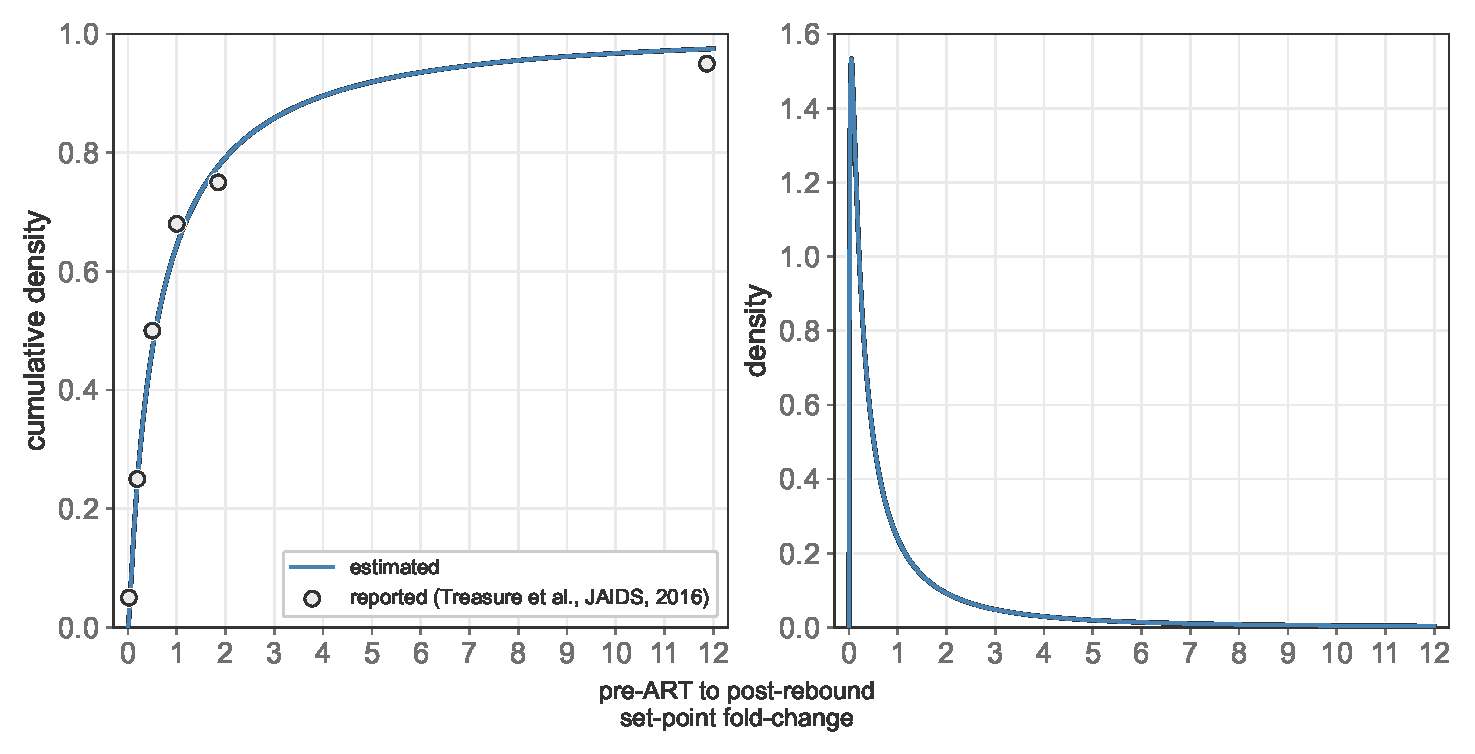
\includegraphics[width=0.75\textwidth]{../figures/eps/pre_post_art_spvl.eps}
    \caption{\textbf{Estimated scaling factor between pre-treatment set-point and post-rebound set-point}. A) Reported quantiles in Treasure et al., JAIDS, 2016 \protect\citesupp{treasure2016} (dots) and estimated cumulative density of the best-fit lognormal distribution found by minimizing squared error. B) Probability density function of the best-fit lognormal distribution shown in (A).} 
    \label{fig:pre_post_art_spvl} % Used for referencing
\end{figure}

During the waiting time between ART stop until rebound initiation, viral load is assumed to remain constant at its value when ART was stopped. To account for the fact that viral rebound in this model can begin from any arbitrary viral load, we assumed that following dynamics when not on treatment and outside of the waiting period between ART and rebound initiation: 1) when treatment is ceased at a viral load below the post-treatment set-point it will grow at the early exponential growth rate until viral load peak followed by decay at the post-peak decay rate until the set-point, 2) when treatment is ceased at a viral load above the post-treatment set-point but below the peak value it will randomly be assigned, based on the relative values of the early exponential growth rate and the post-peak decay rate, to either grow to the peak at the early exponential growth rate or decay to the post-treatment set-point at the post-peak decay rate, 3) when treatment is ceased at a viral load above the peak value (which can occur as individual-level parameters are drawn from independent distributions) it will decay at the post-peak decay rate until the post-treatment set-point, and 4) once at post-treatment set-point following growth to the peak and subsequent decay the viral load will remain constant. 

For all analyses we use a time-step of one day. When estimating the rate of treatment cessation from observed RCCS viral load trajectories, we used parameters for NNRTI-based ART regimens. Of 109 paired viral load trajectories, the follow-up observation was taken during RCCS round 19 or earlier in 91 (83\%). During this time frame, NNRTI-based regimens were the predominant ART regimen in the region \cite{martin2026}. However, as our primary interest when forward projecting viral dynamics under fixed rates of treatment cessation was to quantify the expected burden of transmission from individuals with low-level viremia under contemporary treatment regimens we used non-NNRTI-based regimens. We note that while the predominant treatment regimen in the RCCS at present is based on dolutegravir (DTG), an integrase inhibitor, the estimated rates of viral decay for non-NNRTI-based regimens reported in \cite{andrade2013} are for raltegravir (RAL), which is also an integrase inhibitor. However, the rate of viral load decay have previously been shown to be comparable between DTG and RAL \citesupp{vanlunzen2012, markowitz2007}. As such, we used the rates reported for RAL-based regimens in \cite{andrade2013} for consistency with our NNRTI-based parameterization. All model parameters are summarized in \textbf{Table \ref{table:simulation_parameters}}.

\begin{table}[hp]
\centering
\caption{\textbf{Summary of parameters used in the viral load simulation model.} Parameters chosen to match non-nucleoside reverse transcriptase inhibitor (NNRTI) dynamics as most Rakai Community Cohort Study viral load data was collected during NNRTI-based first-line regimne use. The $\sim$ symbol indicates randomly sampling from a given distribution or vector (with replacement). Equivalent parameterization of the Gamma distribution in terms of mean and standard deviation and $\alpha$ and $\beta$ are provided for convenience. Simulated individuals are indexed with the subscript $l$.}
\footnotesize
\begin{tabular}{lp{0.40\textwidth}p{0.12\textwidth}L{0.30\textwidth}}
\toprule
\textbf{Parameter} & \textbf{Description} & \textbf{Unit} & \textbf{Value} \\
\midrule
$N_l$ & Number of simulated trajectories per iteration & 1 & 100 \\
$V_{sp,l}$ & Pre-treatment viral set-point & copies/mL & Fit to pre-treatment RCCS data. \newline $\sim 10^{\text{Normal}(\mu=4.1, \sigma=0.7)}$ \\
$V_{sp,l}$ & Post-rebound viral set-point & copies/mL & Fit to pre-treatment RCCS data adjusted downwards as in \citesupp{treasure2016}. \newline $\sim V_{sp,l}\text{Lognormal}(\mu=-0.57, \sigma=1.56)$ \\
$V_{l,0}$ & Viral load at $t=0$ & copies/mL & Drawn from RCCS survey visits from individuals self-reported ART use wiht viral load data available at survey $k$ and $k+1$ and viral load between 200 and 1,000 copies/mL at $k$. \newline
$\sim V_{i,k}$ \\
$d_{1,l}$ & First-phase decay rate while on treatment & days$^{-1}$ & Extracted from 
\cite{andrade2013} \newline
$\sim$Gamma($\mu=$0.6, $\sigma=$0.05)  \newline
$\sim$Gamma($\alpha=$144, $\beta=$240) \\
$d_{2,l}$ & Second-phase decay rate while on treatment & days$^{-1}$ & Extracted from 
\cite{andrade2013} \newline
$\sim$Gamma($\mu=$0.07, $\sigma=$0.03) \newline
$\sim$Gamma($\alpha=$5.44, $\beta=$77.78) \\
$a_l$ & Fraction of viral load subject to second-phase decay while on treatment. & --
& Extracted from 
\cite{andrade2013} \\
&$\qquad$ - for INSTI: & & 
$\sim$Gamma($\mu=1.5\times10^{-3}$, $\sigma=4.5\times10^{-4}$) \newline
$\sim$Gamma($\alpha=$11.11, $\beta=$7407.41) \\
&$\qquad$ - for NNRTI: && 
$\sim$Gamma($\mu=2.5\times10^{-2}$, $\sigma=7.5\times10^{-4}$) \newline
$\sim$Gamma($\alpha=$11.11, $\beta=$444.44) \\
$r_l$ & Viral growth rate while off treatment & days$^{-1}$ &
Estimated \newline
$\sim0.53e^{\text{Normal}(\mu=0\text{, }\sigma=0.34)}$ \\
$\Delta_{p,l}$ & Proportional difference between post-treatment viral set-point and peak viral load while off treatment. & --
&
Estimated \newline
$\sim6.55e^{\text{Normal}(\mu=0\text{, }\sigma=1.99)}$ \\
$\delta_l$ & Decay rate from peak viral load to post-treatment set-point while off treatment & days$^{-1}$ &
Estimated \newline
$\sim0.32e^{\text{Normal}(\mu=0\text{, }\sigma=1.67)}$ \\
$T_{w,l}$ & Waiting time between ART interruption and viral rebound initiation & days & Estimated \newline $\sim 5.79e^{\text{Normal}(\mu=0, \sigma=0.71)}$ \\
$x_{l,0}$ & Treatment status (on treatment: $x_{l,0}=1$) at $t=0$. & --
&
Assumed \newline
1 \\
$w^\text{cease}$ & Rate of treatment cessation & days$^{-1}$ &
Fit to paired RCCS viral load observations from participants self-reporting treatment, \newline
median (95\% CI): 0.26 (0.19, 0.36), \newline  or 
fixed such that 25 through 60\% \newline
of people cease treatment 
annually. \\
\midrule
\textbf{Trans. param.} & \textbf{Description} & \textbf{Unit} & \textbf{Value} \\
$V_{rp,l}$ & Post-treatment viral set-point & copies/mL &
Fit to pre-treatment RCCS data, adjusted to account for reduced post-treatment set-point \citesupp{treasure2016}. \newline
$\sim 0.5\times V_{sp,l}$ \\
\bottomrule
\end{tabular}
\label{table:simulation_parameters}
\end{table}

We first used this model to estimate the remaining free parameter, the rate of treatment cessation ($\omega^\text{cease}$) from observed viral load trajectories of RCCS participants, through simulation-based inference. We assume this rate is shared between all simulated individuals. Specifically, we identified paired viral load measurements from individuals self-reporting treatment ($\text{ART}_{i,k}=1$) with available viral load data at round $k$ and round $k+1$ ($v_{i,k} \neq \text{NULL}, v_{i,k+1} \neq \text{NULL}$). We used only the first available $k,k+1$ pair for each individual. Each $i,k$, $i,k+1$ pair is associated with a time of initial and follow-up observation $c_{i,k}$, $c_{i,k+1}$ separated by duration $t_{i,k+1}$. We let $L$ represent the set of all $i,k$ pairs that satisfy these conditions. To perform simulated-based inference using this model, we first calculated the quintiles of log$_{10}$ viral load observations, $v_{i,k+1}$, $Q_{1...4}$ and assigned each $v_{i,k+1}$ to a quintet, $z_i=1,2,3,4,\text{ or } 5$. For a given value of $\omega^\text{cease}$ we can simulate viral load trajectories and, at each time step of the simulation, calculate the probability mass of simulated viral load values that fall into each quintet, $P(q_{1...5}|t)$. The likelihood of that $\omega^\text{cease}$ value is then equal to the sum of the probabilities of each observed quintet, $\sum_{i,k \in L}P(q_{z_i} | t_{i,k+1})$. We performed parameter inference using Markov Chain Monte carlo with a Metropolis-Hastings acceptance algorithm and 100 simulated trajectories for each iteration. At each iteration, new individual-level values were drawn for initial viral load, post-treatment set-point viral load, and viral decay and growth in the presence and absence of treatment, respectively. A uniform prior was used for $\omega^\text{cease}$. Chains were run for 25,000 iterations and the first 50\% of the chain discarded as burn-in. Associated trace plots are provided in \textbf{Figure \ref{fig:rccs_omega2_fit}}. A density plot of estimated post burn-in $\omega^\text{cease}$ values is provided in \textbf{Figure \ref{fig:vl_traj}E}. The estimated value of $\omega^\text{cease}$ was \var{q0.5_omega_cease_per_year} (95\% CI: \var{q0.025_omega_cease_per_year}, \var{q0.975_omega_cease_per_year}) per year

\begin{figure}[!ht] % h! forces the figure to stay "here"
    \centering
    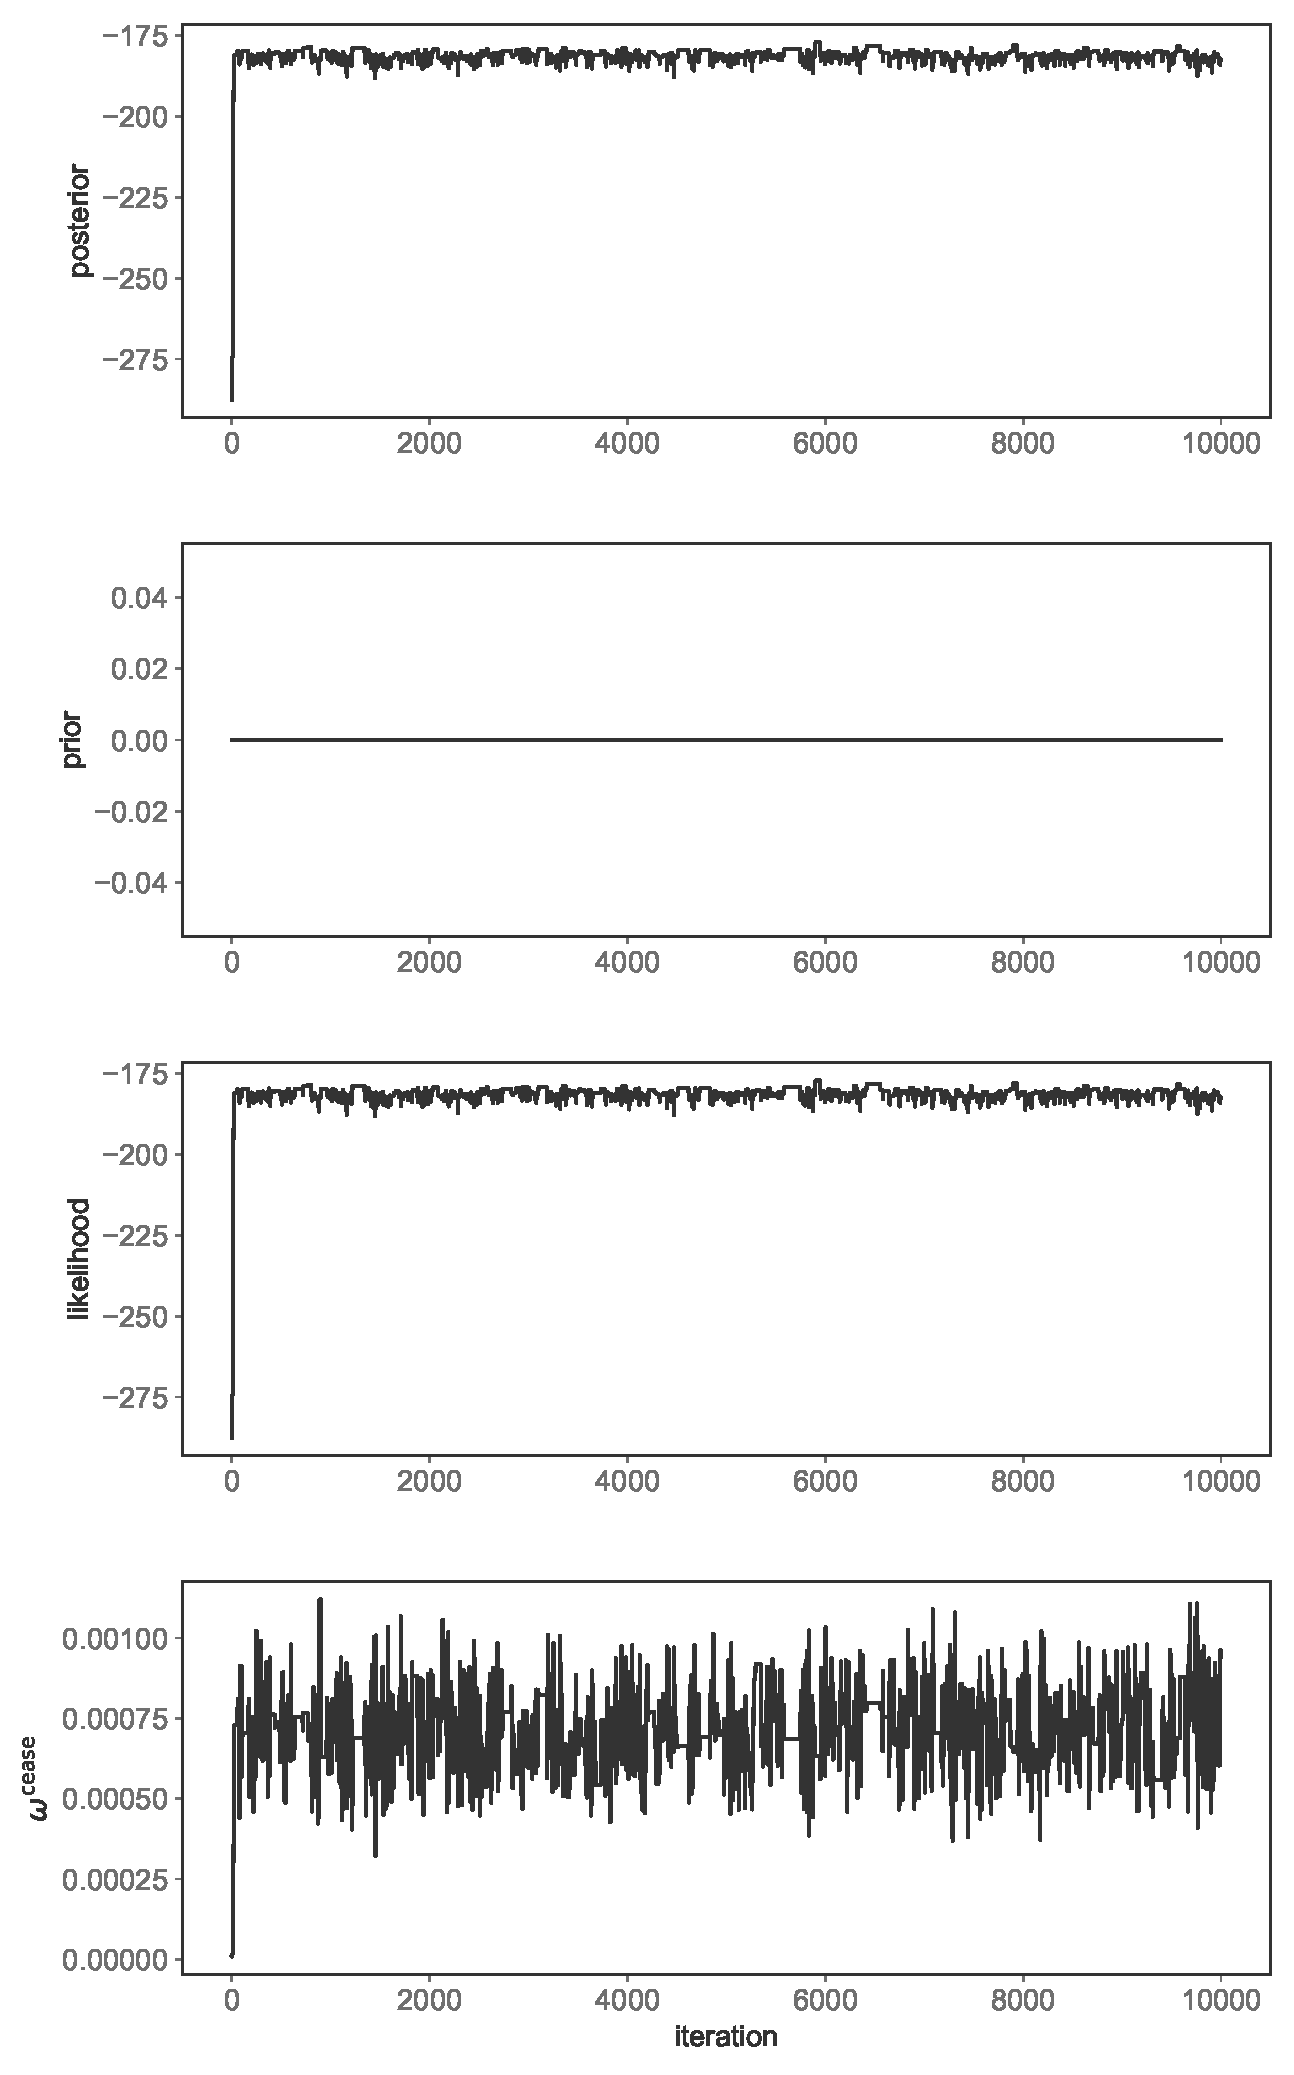
\includegraphics[width=0.75\textwidth]{../figures/eps/rccs_omega_fit_trace.eps}
    \caption{\textbf{Estimated rate of treatment cessation from paired viral load measurements of Rakai Community Cohort Study participants on treatment, \protect \var{r1_minYear}-\protect \var{r19_maxYear}.} }
    \label{fig:rccs_omega2_fit} % Used for referencing
\end{figure}

Using the estimated rate of treatment cessation from paired viral load measurements, we next aimed to quantify the expected number of transmissions from a cohort of individuals with low-level viremia and on effective therapy at baseline. To do this, we took a random sample of 1,000 post-burn MCMC iterations each with an associated value of $\omega^\text{cease}$ and 100 simulated viral load trajectories ($N_l$). Each of these posterior draws was paired with a posterior draw of estimated $\rho_\text{prod.}, \rho_\text{est.},\text{ and } c$ values (\textbf{Statistical model relating viral load to transmission rate}, Model \#1: Main analysis). For a given posterior sample ($p$) of 100 simulated viral load trajectories ($l$) and 100 ${\rho_\text{prod.}}, \rho_\text{est.},\text{ and } c$ values, we calculated the expected cumulative number of transmissions at each time point in the simulation, $y$. We assume that sexual acts occur at a rate of $f = 108$ per year \cite{quinn2000}. Based on \textbf{Eq. \ref{eq:prob_intra_trans}}, given a viral load for simulated trajectory $l$ at time $t$ ($V_{l,t}$) and parameters for the virion establishment model the transmission rate per year is given by $f\rho_\text{prod.}(1 - (1 - \rho_\text{est.})^{cV_{l,t}}$. The expected number of transmissions over a one day time-step of the simulation is therefore $(\frac{f}{365})\rho_\text{prod.}(1 - (1 - \rho_\text{est.})^{cV}$. We can then calculated the cumulative number of transmissions that have occurred among the $N_l$ simulated trajectories up to time $T$ in the simulation as the sum of the expected number at each time step, 

\begin{align}
y_{p}(T) = \sum_{l=1}^{N_l = 100}\sum_{t=0}^T \frac{f}{365}{\rho_\text{prod.}}_p\left(1 - (1 - {\rho_\text{est.}}_p)^{c_pV_{l,t}}\right).
\end{align}

We note that this approach assumes that all sexual acts are with HIV negative partners. It does not account for the fact that some sexual acts may be with HIV seropositive individuals and therefore even if transmission occurs will not result in an incident HIV infection. Particularly given the fact that HIV seroprevalence is on the order of 40\% in some RCCS communities \citesupp{chang2016} this represents an upper bound of the expected transmissions in real-world settings. Representative simulated viral load trajectories are shown in \textbf{Figure \ref{fig:vl_traj}C}. The estimated cumulative number of HIV transmissions at each time-point over a one-year span is provided in \textbf{Figure \ref{fig:vl_traj}D}. 

Finally, we used this model to similarly estimate the expected number of transmissions from cohorts of individuals who have low-level viremia and are on effective treatment at baseline across alternative fixed values of the treatment cessation rate, $\omega^\text{cease}$. Specifically, we simulated sets of 1,000 $\times$ 100 viral load trajectories to pair with 1,000 posterior samples of $\rho_\text{prod.}$, $\rho_\text{est.}$, and $c$ as above under values of $\omega^\text{cease}$ such that the probability of treatment cessation over a one-year period ($\rho_\text{cease} = 1 - e^{\omega^\text{cease}\times 365.25}$) was 25, 30, 35, 40, 45, 50, 55, and 60\%. The expected number of transmissions over a one year period with trajectories simulated under each of these parameter values was calculated in the same manner as above. These estimates are provided in \textbf{Figure \ref{fig:vl_traj}E}.


\subsection*{Statistical model to estimate the prevalence of low-level viremia}
Our interest is in estimating the proportion of the overall population with HIV viral loads in each of four categories: $<40$ copies/mL, 40-200 copies/mL, 200-1,000 copies/mL, and $>1,000$ copies/mL in each of the five RCCS survey rounds with cohort-wide viral load monitoring between \var{r16_minDate} and \var{r20_maxDate} (survey rounds 16 through 20, \textbf{Figure \ref{fig:study_participants}}). However, we must account for a small amount of missing HIV serostatus and viral load data over this time frame. Our overall approach is to: 1) calculate the proportion of individuals that are HIV seropositive among those with measured HIV serostatus in each RCCS survey and 2) calculate the proportion of measured viral loads among HIV seropositive individuals belonging to each of the four viral load categories in each RCCS survey. Then, we calculate the product of these two quantities to estimate the proportion of the overall population in that survey in each HIV viral load category. Because levels of missingness and viral load distributions differ by demographic characteristics (e.g. age, sex, type of community of residence) we calculate each of these quantities within population sub-groups and then use post-stratification weighting to generate population-wide estimates. 

The assumption of this approach are as follows:

\begin{itemize}
    \item Within strata defined by sex, categorical age (15-24, 25-34, 35-49), and community type (agrarian, fishing, trading), data can be considered to be missing at random (that is, there is no further correlation between the value of viral load and the probability it is missing) 
    \item The proportion of individuals in the population belonging to each strata in each survey round is equal to the proportion of study participants in that strata in each survey round
    \item The prevalence of HIV seropositivity within a given survey period and strata is equal to the measured proportion of HIV seropositive participants among those with HIV serological data in that survey round and strata
    \item The relative proportion of individuals in a given viral load category among those with HIV in a given survey period and stata is equal to the measured proportion among HIV seropositive participants in that survey round and strata.
\end{itemize}

Formally, we first enumerate the $D$ demographic groups (strata) for convenience and let $d_{i,k}$ be the strata for participant $i$ in survey $k$ (because people age and can move communities a participant may be a member of different strata at different RCCS surveys). We let $N^d_{x,k}$ be the number of participants in strata $x$ in round $k$. We estimate HIV seroprevalence in strata $x$ in round $k$, $H_{x,k}$, as the proportion of measured HIV serostatuses in strata $x$ in round $k$ that are seropositive, $H_{x,k} = \frac{\sum_i \sum_{k:d_{i,k}=x, h_{i,k} \neq \text{NULL}}h_{i,k}}{\sum_i \sum_{k:d_{i,k}=x, h_{i,k} \neq \text{NULL}} 1}$. Here, $h_{i,k}$ is the HIV serostatus of participant $i$ in round $k$. In this notation $\sum_i\sum_{k:d_{i,k}=x, h_{i,k} \neq \text{NULL}}$ sums over all participants ($i$) and survey rounds ($k$) such that participant $i$ participated in round $k$ is in strata $x$ and has HIV serostatus data ($h_{i,k} \neq \text{NULL}$).

Similarly, we can estimate the prevalence of a given viral load category $z$ among those with HIV in strata $x$ in round $k$, $C^z_{x,k}$, as the proportion of measured HIV viral loads in strata $x$ in round $k$ that are in that category. As defined in \textbf{Table \ref{table:rccs_vars}} each viral load category is associated with a binary data variable e.g. $<40$ copies/mL: $\text{BD}_{i,K}$, 40-200 copies/mL: $\text{MLV}_{i,k}$, 200-1,000 copies/mL: $\text{LLV}_{i,k}$, $>1,000$ copies/mL: $\text{VIR}_{i,k}$. In this notation $C^\text{BD}_{x,k}$ would be the proportion of measured viral loads in strata $x$ in round $k$ that are $<40$ copies/mL. Thus, for each of $z \in \{\text{BD}, \text{MLV}, \text{LLV}, \text{VIR}\}$ we have $C^z_{x,k} = \frac{\sum_i \sum_{k:d_{i,k}=x, v_{i,k} \neq \text{NULL}} z_{i,k}}{\sum_i \sum_{k:d_{i,k}=x, v_{i,k} \neq \text{NULL}} 1}$. Here, $v_{i,k}$ is the measured viral load of participant $i$ in survey $k$ which is assumed to be NULL for HIV seroengative individuals or those with missing HIV serostatus data. 

We can then calculate the prevalence of being seropositive and in a given viral load category among all participants within a strata, $\zeta^z_{x,k}$, by taking the product of the estimated prevalence of that category among those with HIV and the estimated prevalence of HIV seropositivity, $\zeta^z_{x,k} = H_{x,k}\times C^z_{x,k}$. Finally, to estimate the prevalence of a given viral load category among all participants in a given survey, we take the mean of strata-specific estimates weighted by the number of participants in that strata, $\frac{\sum_{x=1}^D \zeta^z_{x,k}\times N^d_{x,k} }{N^d_{x,k} }$. These estimates are presented in \textbf{Figures \ref{fig:study_participants}B,C}. 

We also wished to calculate the specific prevalence of low-level viremia among all participants and among those people with HIV with viral load $>200$ copies/mL accounting not just for missing HIV serostatus and viral load data but also for the fact that RCCS participants can participate in multiple surveys and their HIV serostatus and viral load across surveys may be correlated. To do so, we use Bayesian mixed-effects logistic regression with strata-round specific effects and individual-level random effects. We model three distinct outcomes: HIV seropositivity among measured viral loads ($H$), HIV viral load greater than 200 among those people with HIV and viral load data ($C^{\text{LLV}|\text{VIR}}$), and HIV viral load between 200 and 1000 among those people with HIV with measured viral load greater than 200 ($C^\text{LLV}$). From these regression equations, we attain strata-round specific estimates for the probability of each outcome that account for individual-level random effects (and their associated uncertainty) but do not depend on the specific random effects observed in the sample by integrating over the estimated random-effects distribution. This also accounts for the fact that random effects that are mean 0 on the logit scale are not mean 0 on the natural (probability) scale. Finally, using the strata-round specific weights as above and the strata-round specific probability of each outcome, we can estimated the desired quantities: the prevalence of low-level viremia among all participants and the prevalence of low-level viremia among those participants with HIV with viral load $>200$ copies/mL. 

Specifically, we model the log-odds of a positive HIV serostatus (among those with data, $h$), as having a population mean value ($\alpha_{\text{HIV+}}$), a round-stata-specific fixed effects (vector of length $5 \times D$, $\beta_{\text{HIV+},[k \times d_{i,k}]}$), and an individual-level random effect with standard deviation $\sigma_{\text{HIV+}}$. Therefore, we assume individual $i$ in survey round $k$ has a positive HIV serostatus (given they were tested, $h_{i,k}$) drawn from the distribution

\begin{equation}
\begin{split}
(h_{i,k} | k \in [16, 20], h_{i,k} \neq \text{NULL}) &\sim \text{Bernoulli}(\mu_{\text{HIV+},i}) \\
\text{logit}(\mu_{\text{HIV+},i}) &= \alpha_{\text{HIV+}} + \beta_{\text{HIV+},[k \times d_{i,k}]} + \sigma_\text{HIV+}\epsilon_{\text{HIV+},i} 
\end{split}
\end{equation}

with priors 
\begin{equation}
\begin{split}
\alpha_{\text{HIV+}} &\sim \text{Normal}(\mu=0,\sigma=2) \\
\beta_{\text{HIV+}} &\sim \text{stz-Normal}(\mu=0,\sigma=2) \\
\sigma_{\text{HIV+}} &\sim \text{Half-Normal}(\mu=0,\sigma=1)\\
\epsilon_{\text{HIV+}} &\sim \text{Normal}(\mu=0,\sigma=1) 
\end{split}
\end{equation}

%Here, $\beta_{1}$ is a vector of coefficients for each of $5 \times D$ strata-round coefficients, with $-15$ in the index as $k$ is the round index and we only estimate coefficients for RCCS survey rounds 16 through 20. 
We assume a $\text{stz-Normal}$ (sum-to-zero Normal) prior to ensure identifiability.

Based on this model, we would formally estimate a strata-round specific prevalence of HIV by integrating over the individual level random effects, $H_{x,k} = \int_{-\infty}^\infty\text{inv-logit}\left(\alpha_{\text{HIV+}} + \beta_{{\text{HIV+}},[x\times k]} + u\right)\text{Normal}(u | \mu=0,\sigma=\sigma_{\text{HIV+}})du$ where $\text{Normal}(u | \mu=0,\sigma=\sigma_{\text{HIV+}})$ evaluates the Normal distribution density with mean 0 and standard deviation $\sigma_{\text{HIV+}}$ at the value of $u$. We approximate this integration using Monte Carlo integration, taking 100 random samples from the estimated random-effects distribution ($u_{1,r} \sim N(0, \sigma_{\text{HIV+}}^2)$) and calculating $H_{x,k}$ for each posterior sample based on these random samples, $H_{x,k} = \frac{\sum_{r=1}^{r=100}\text{inv-logit}\left(\alpha_{\text{HIV+}} + \beta_{{\text{HIV+}},[x\times k]} + u_{{\text{HIV+}},r}\right)}{100}$.

We similarly fit logistic regressions for the outcome of viral loads $>200$ ($(\text{LLV}_{i,k}|\text{VIR}_{i,k})$) among HIV seropositive individuals with viral load data 

\begin{equation}
\begin{split}
((\text{LLV}_{i,k}|\text{VIR}_{i,k}) | k \in [16,20], v_{i,k} \neq \text{NULL}) &\sim \text{Bernoulli}(\mu_{\text{200+},i}) \\
\text{logit}(\mu_{\text{200+},i}) &= \alpha_{\text{200+}} + \beta_{\text{200+},[k \times d_{i,k}]} + \sigma_\text{200+}\epsilon_{\text{200+},i}
\end{split}
\end{equation}
with priors
\begin{equation}
\begin{split}
\alpha_\text{200+} &\sim \text{Normal}(\mu=0,\sigma=2) \\
\beta_\text{200+} &\sim \text{stz-Normal}(\mu=0,\sigma=2) \\
\sigma_\text{200+} &\sim \text{Half-Normal}(\mu=0,\sigma=1)\\
\epsilon_\text{200+} &\sim \text{Normal}(\mu=0,\sigma=1)
\end{split}
\end{equation}

and final prevalence estimate
\begin{equation}
\begin{split}
u_\text{200+} &\sim \text{Normal}(\mu=0,\sigma=\sigma_\text{200+}) \\
C^{(\text{LLV}_{i,k}|\text{VIR}_{i,k})}_{x,k} &= \frac{\sum_{r=1}^{r=100}\text{inv-logit}\left(\alpha_\text{200+} + \beta_{\text{200+},[x\times k]} + u_{\text{200+},r}\right)}{100}.
\end{split}
\end{equation}

For the outcome of between 200 and 100 ($\text{LLV}_{i,k}$) among HIV seropositive individuals with viral load data, we apply an analogous approach

\begin{equation}
\begin{split}
(\text{LLV}_{i,k} | k \in [16,20], v_{i,k} \neq \text{NULL}) &\sim \text{Bernoulli}(\mu_{\text{LLV},i}) \\
\text{logit}(\mu_{\text{LLV},i}) &= \alpha_{\text{LLV}} + \beta_{\text{LLV},[k \times d_{i,k}]} + \sigma_\text{LLV}\epsilon_{\text{LLV},i}
\end{split}
\end{equation}
with priors
\begin{equation}
\begin{split}
\alpha_\text{LLV} &\sim \text{Normal}(\mu=0,\sigma=2) \\
\beta_\text{LLV} &\sim \text{stz-Normal}(\mu=0,\sigma=2) \\
\sigma_\text{LLV} &\sim \text{Half-Normal}(\mu=0,\sigma=1)\\
\epsilon_\text{LLV} &\sim \text{Normal}(\mu=0,\sigma=1) 
\end{split}
\end{equation}

and final prevalence estimate
\begin{equation}
\begin{split}
u_\text{LLV} &\sim \text{Normal}(\mu=0,\sigma=\sigma_\text{LLV}) \\
C^{\text{LLV}}_{x,k} &= \frac{\sum_{r=1}^{r=100}\text{inv-logit}\left(\alpha_\text{LLV} + \beta_{\text{LLV},[x\times k]} + u_{\text{LLV},r}\right)}{100}.
\end{split}
\end{equation}

Based on the estimated prevalence of HIV in each strata-round ($H_{x,k}$), we can calculate the prevalence of low-level viremia among all participants in each strata ($H_{x,k}\times C^\text{LLV}_{x,k}$) and among HIV seropositive individuals with viral loads greater than 200 ($\frac{H_{x,k}\times C^\text{LLV}_{x,k}}{H_{x,k}\times C^{\text{LLV}|\text{VIR}}_{x,k}}$) and use post-stratification weighting as above to generate cohort-wide estimates in each survey round. These estimates are provided in the \textbf{Results} text, \textbf{Low-level viremia in the RCCS and serodifferent couple follow-up}.

Parameter inference was performed using Hamiltonian Monte Carlo in textsc{CmdStan v.2.38.0} \citesupp{cmdstan} accessed through \textsc{CmdStanPy v.1.3.0} \citesupp{cmdstanpy} with four chains of 5,000 iterations (2,500 warm-up and 2,500 sampling).

 
 \clearpage
 
\section*{Supplementary Figures}

\begin{figure}[!ht] 
    \centering
    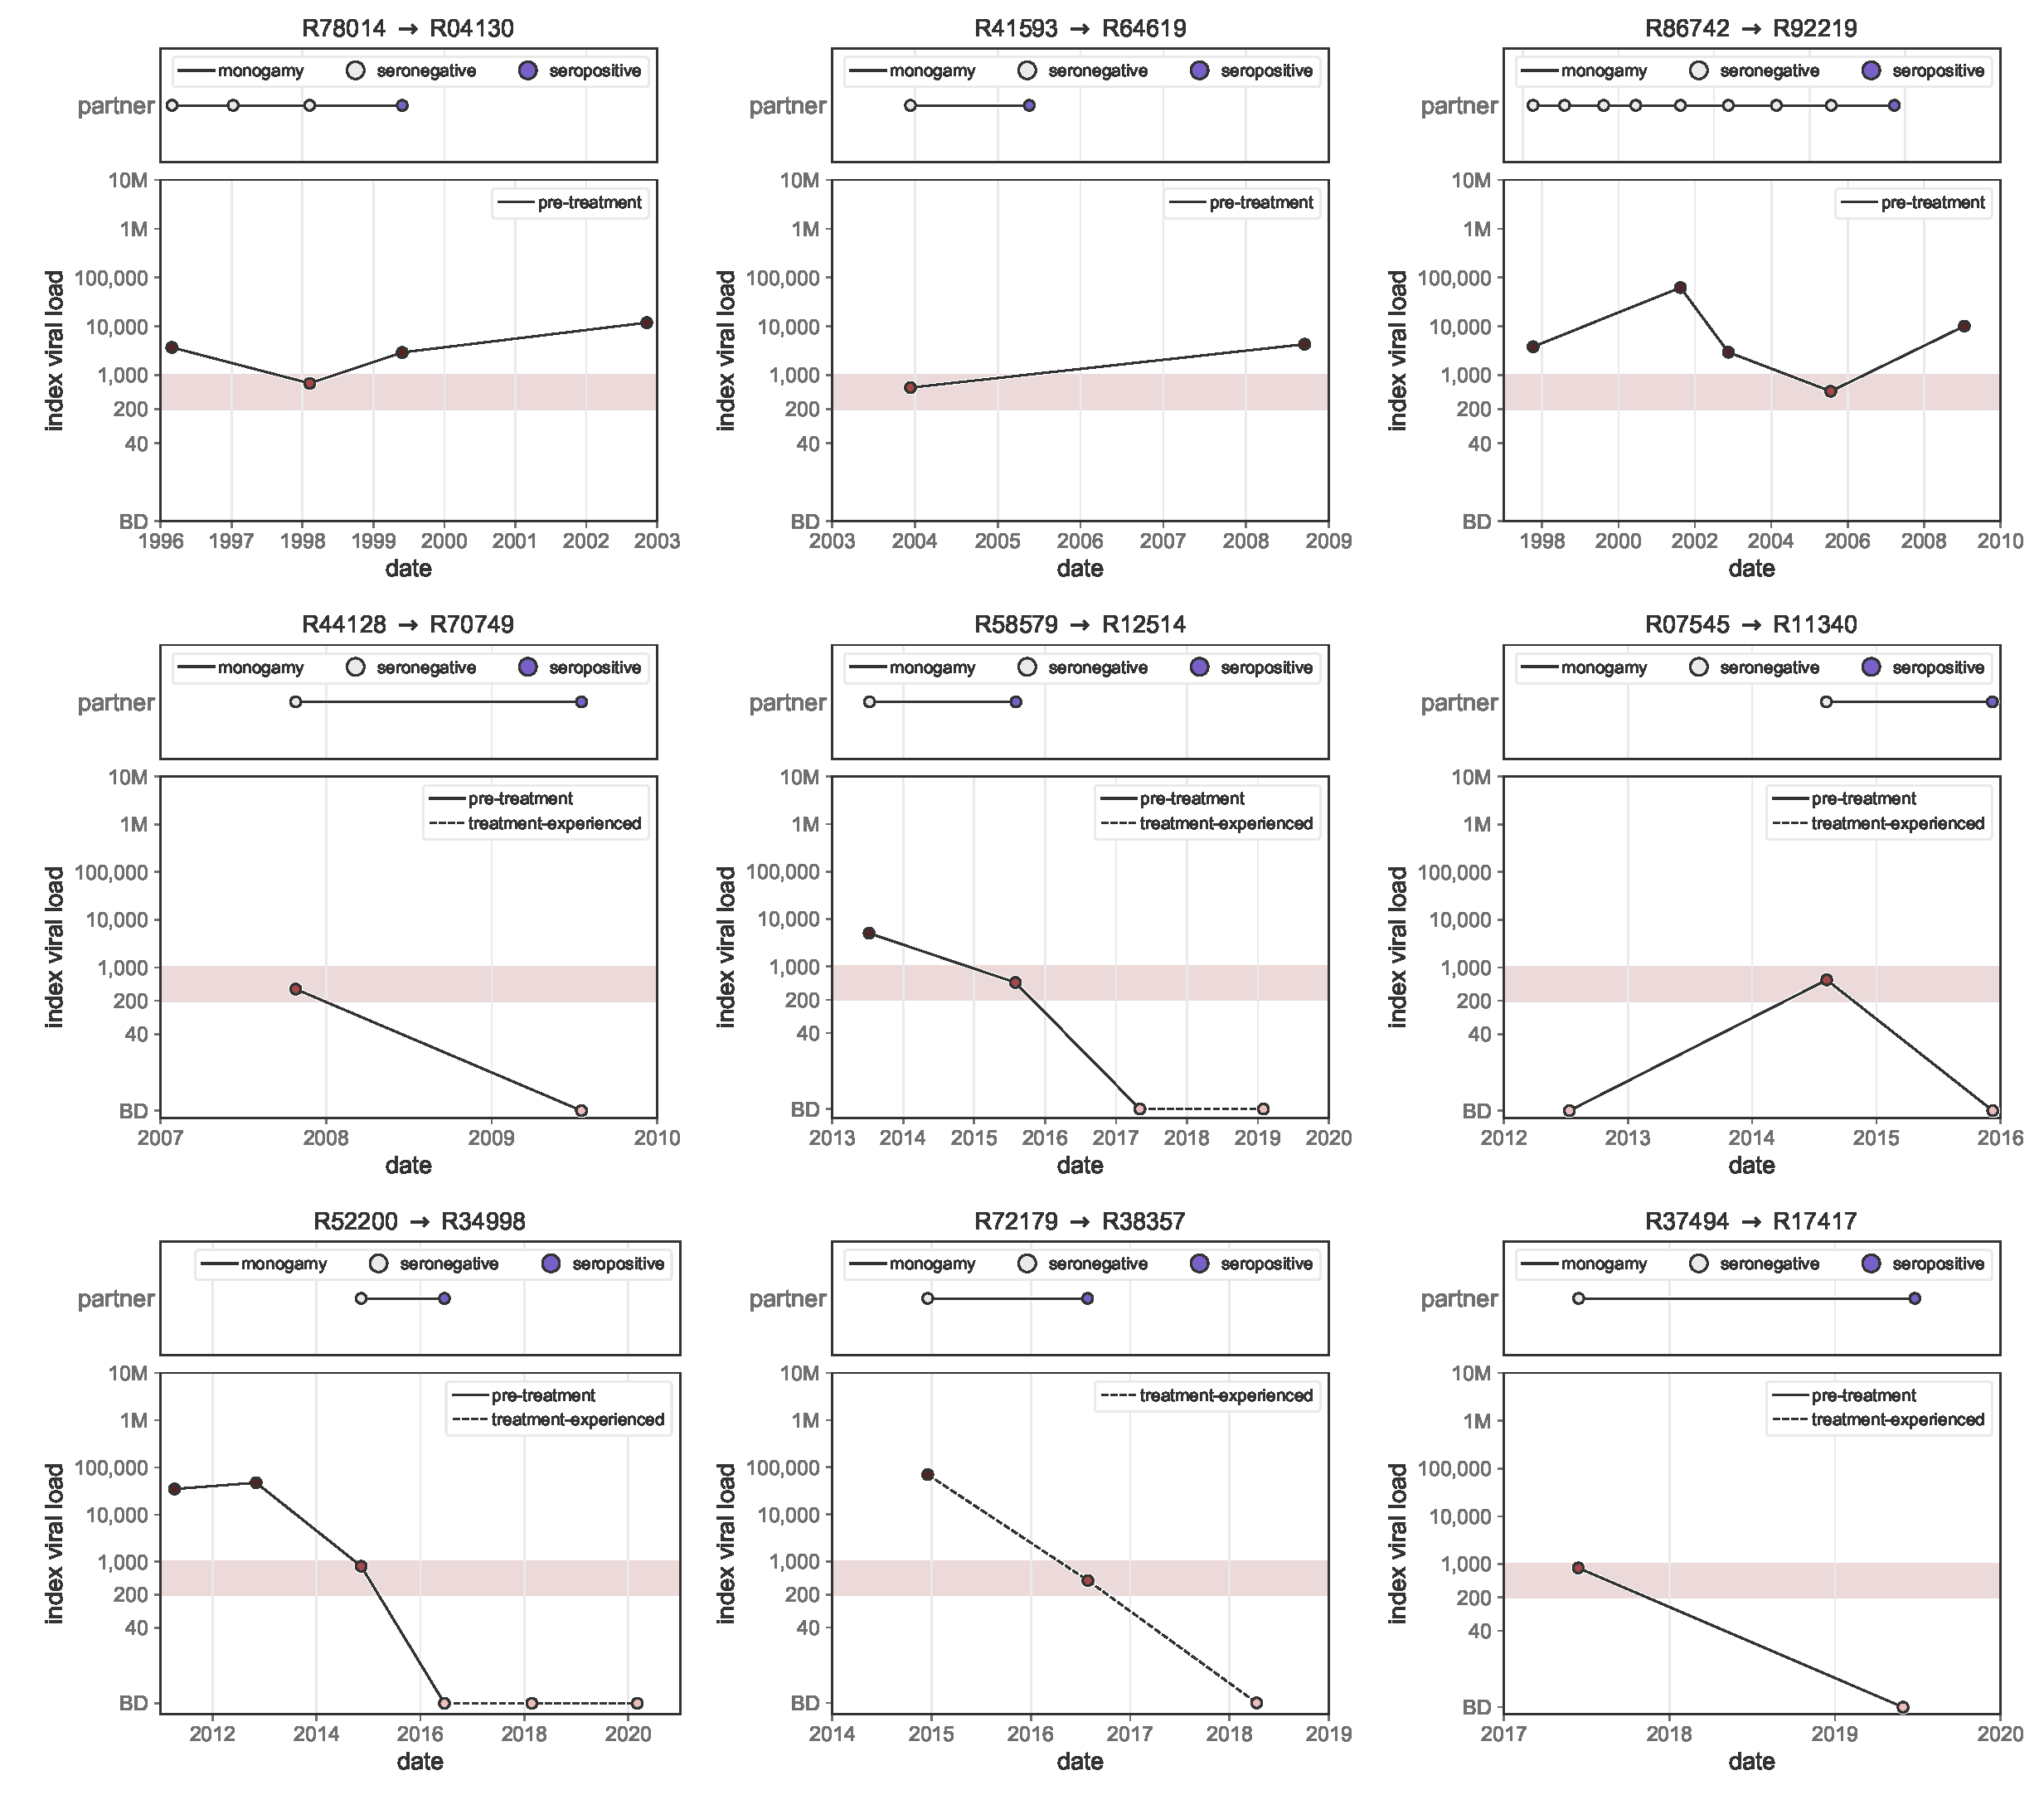
\includegraphics[width=1.0\textwidth]{../figures/eps/select_vl_traj.eps}
    \caption{\protect \textbf{Timing of partner HIV testing and index viral load trajectories of couples with low-level viremia proximal to first partner HIV seropositivity}.}
    \label{fig:select_vl_traj} % Used for referencing
\end{figure}
 \newpage

\begin{figure}[!ht] 
    \centering
    \includegraphics[width=1.0\textwidth]{../figures/pdf/ve_constrained_pairs.pdf}
    \caption{\textbf{Correlation of estimated parameters, Model \#1. Main analysis.} Parameters are as in \textbf{Tables \ref{table:trans_params} and \ref{table:vl_params}}. Includes a random sample of 1,000 posterior draws.}
    \label{fig:main_analysis_correlation} % Used for referencing
\end{figure}
\newpage

\begin{figure}[!ht] 
    \centering
    \includegraphics[width=1.0\textwidth]{../figures/pdf/ve_constrained_estC_pairs.pdf}
    \caption{\textbf{Correlation of estimated parameters, Model \#3. Estimated $c$.} Parameters are as in \textbf{Tables \ref{table:trans_params} and \ref{table:vl_params}}. Uses a Normal($\mu=0, \sigma=5)$ prior on logit($c$) instead of fixing $c=1$. Includes a random sample of 1,000 posterior draws.}
    \label{fig:est_c_correlation} % Used for referencing
\end{figure}
\newpage

   \begin{figure}[!ht] % h! forces the figure to stay "here"
    \centering
    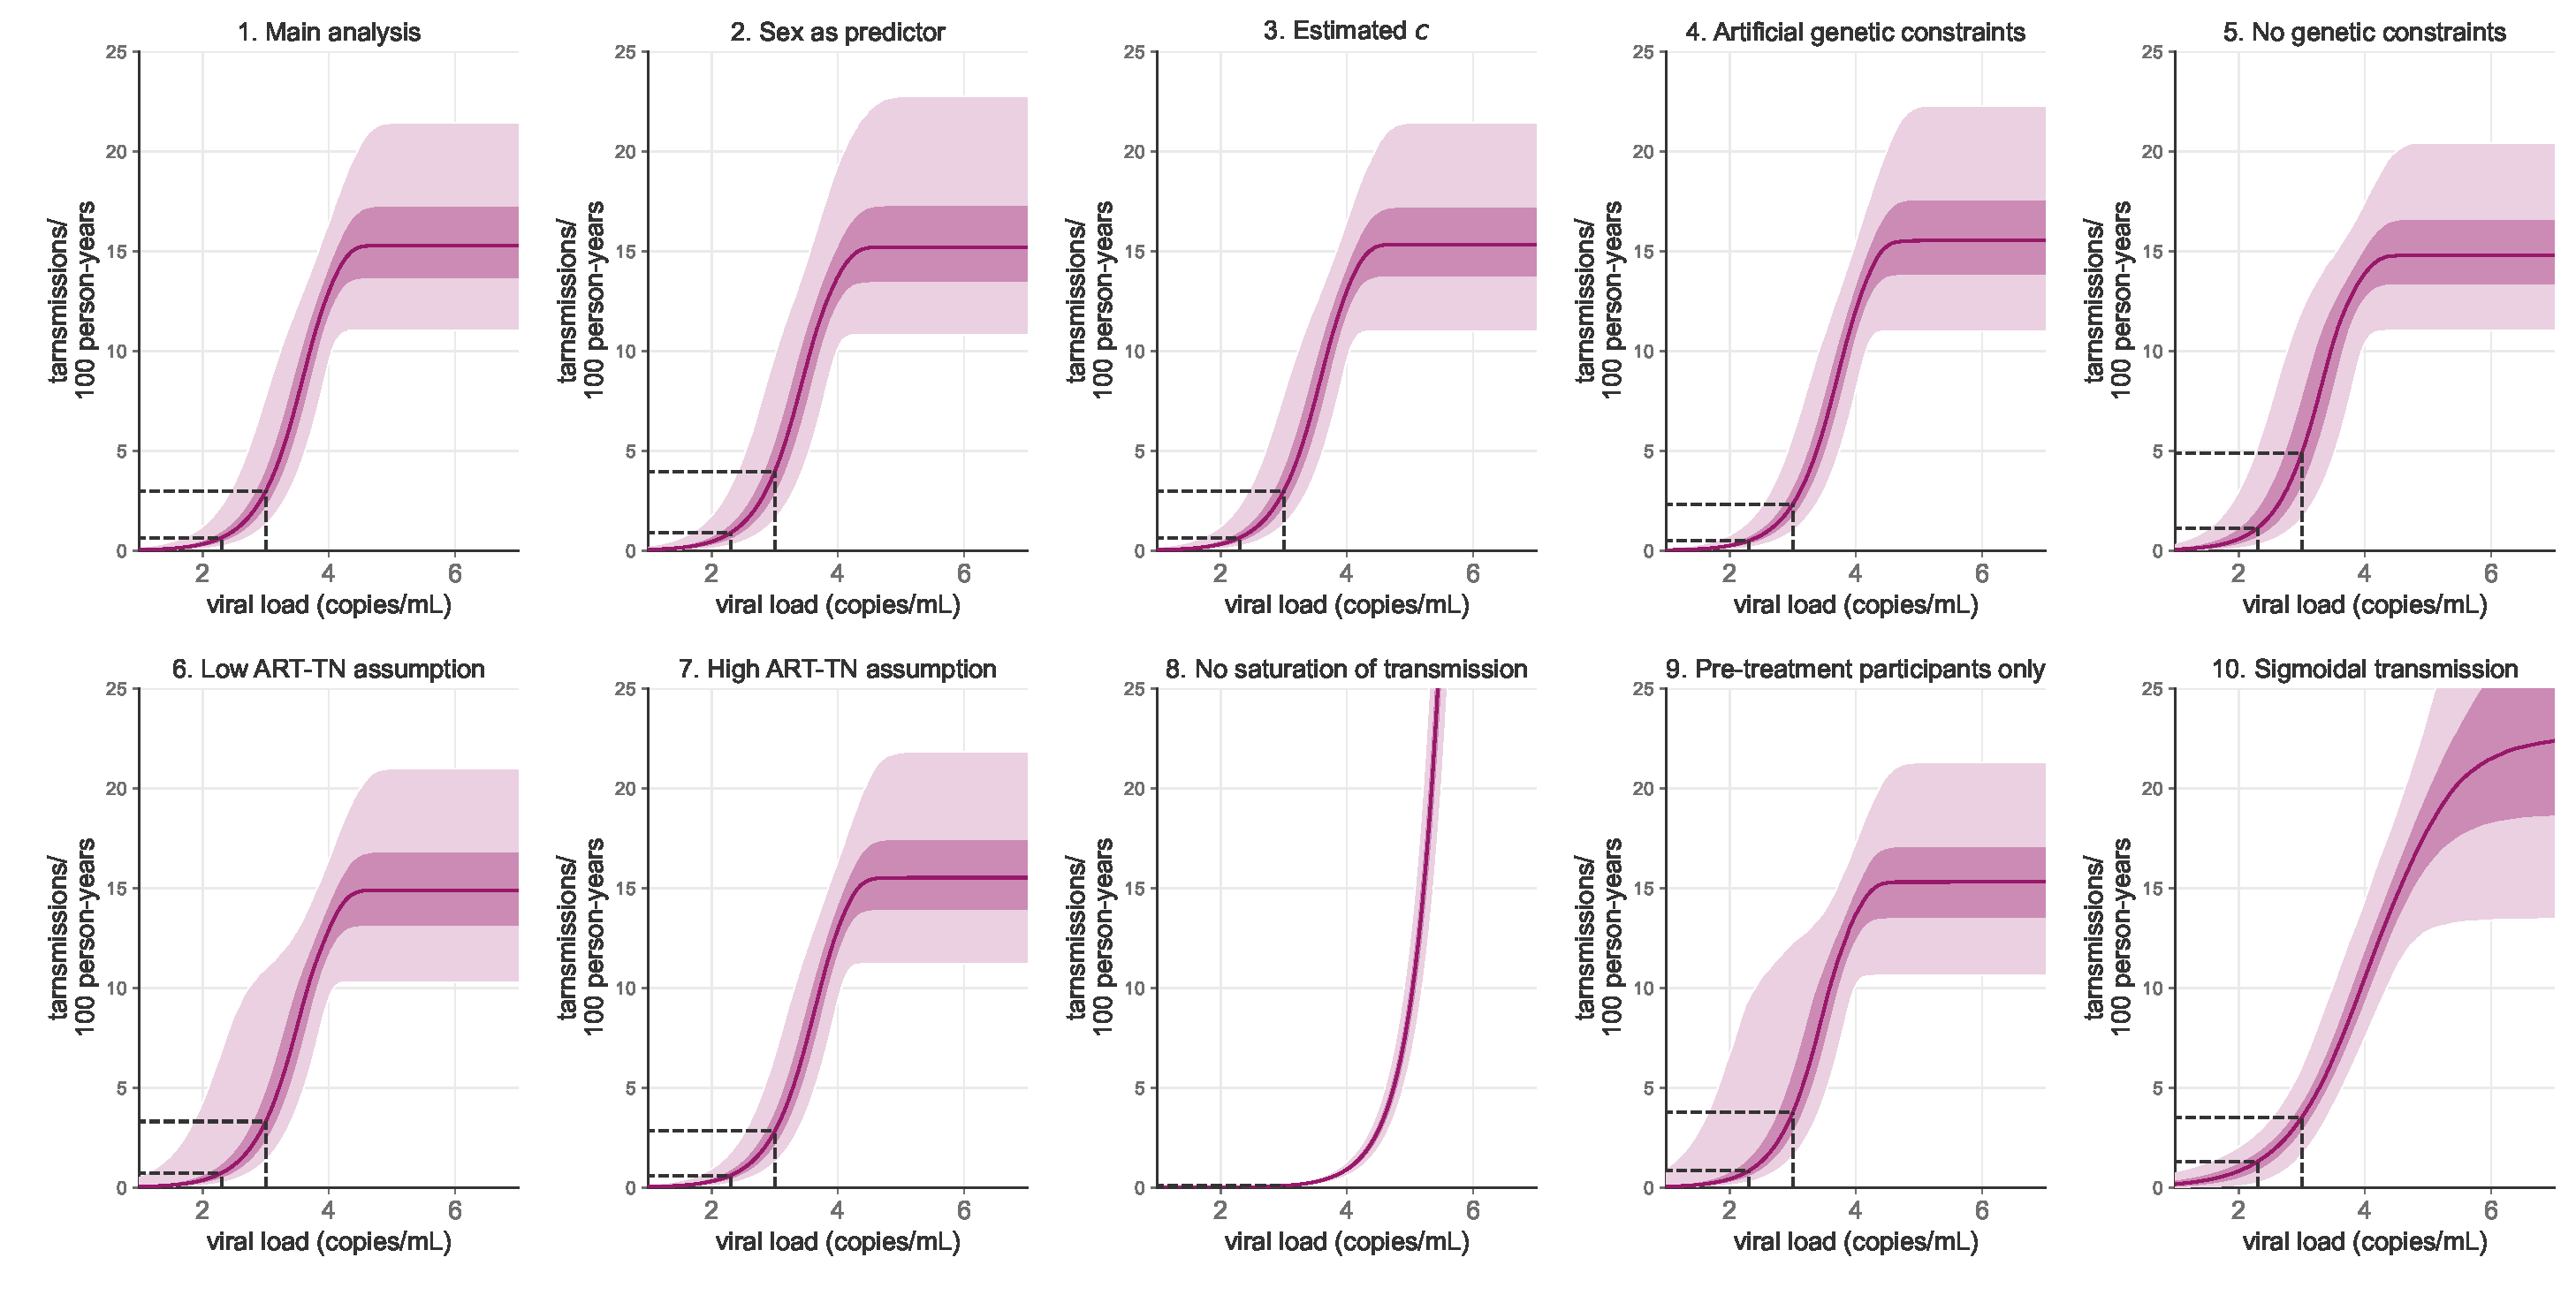
\includegraphics[width=1.0\textwidth]{../figures/eps/intra_couple_trans_risk_all.eps}
    \caption{\textbf{HIV transmission in monogamous serodifferent couples, Rakai Community Cohort Study, \protect \var{r1_minYear}-\protect \var{r19_maxYear}, all models} Estimated transmission rate per 100 person-years as a function of index partner viral load using each of the models fit within this study. Dotted lines highlight the risk of transmission among donors with low-level viremia (200-1,000 copies/mL). Median value is shown as the central line and shading represents the 95\% and 50\% credible interval. }
    \label{fig:intra_couple_trans_risk_all} % Used for referencing
\end{figure}
 \newpage

 


%\begin{figure}[!ht] 
   % \centering
  %  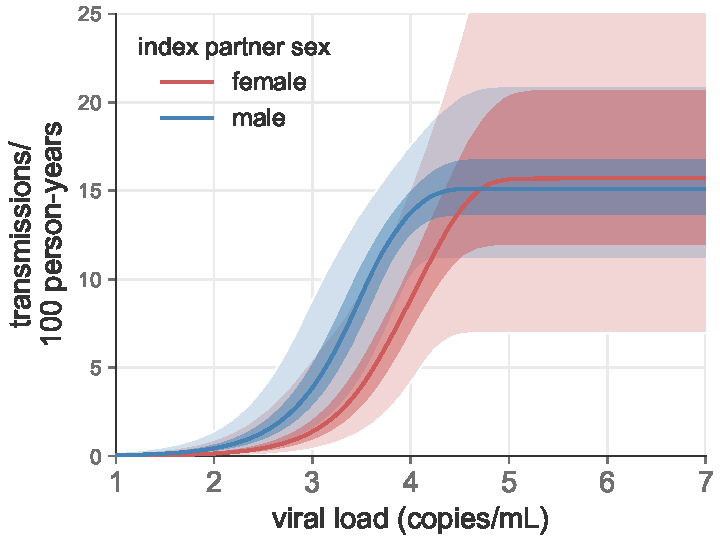
\includegraphics[width=1.0\textwidth]{../figures/pdf/intra_couple_trans_risk_ve_constrained_sex_sex.pdf}
 %   \caption{\textbf{HIV transmission in monogamous serodifferent couples, Rakai Community Cohort Study, \protect \var{r1_minYear}-\protect \var{r19_maxYear}, Model \#2. Sex as predictor.} Estimated transmission rate per 100 person-years as a function of index partner viral load and sex based on logistic regression on $\rho_\text{prod.}$ and $\rho_\text{est.}$. Median value is shown as the central line and shading represents the 95\% and 50\% credible interval. }
    \label{fig:intra_couple_trans_risk_sex} % Used for referencing
%\end{figure}
%\newpage

%\begin{figure}[!ht] 
   % \centering
  %  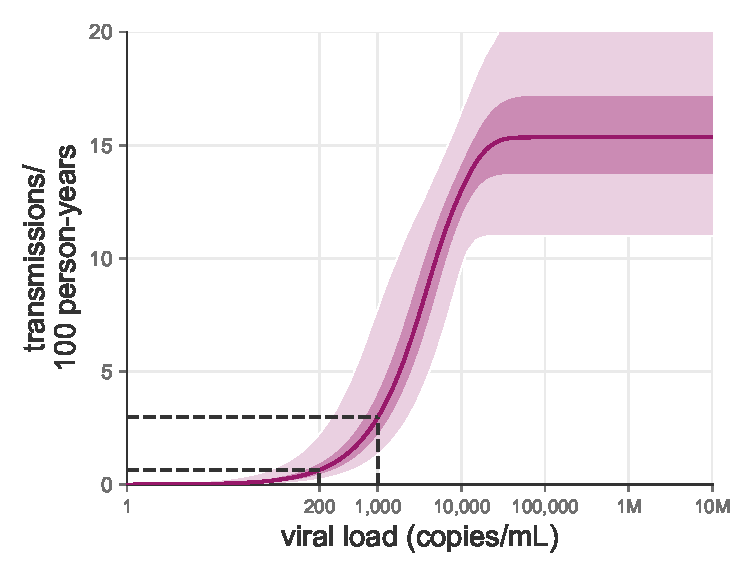
\includegraphics[width=1.0\textwidth]{../figures/eps/intra_couple_trans_risk_ve_constrained_estC.eps}
 %   \caption{\textbf{HIV transmission in monogamous serodifferent couples, Rakai Community Cohort Study, \protect \var{r1_minYear}-\protect \var{r19_maxYear}, Model \#3. Estimated $c$.} Estimated transmission rate per 100 person-years as a function of index partner viral load using a Normal($\mu=0, \sigma=5)$ prior on logit($c$) instead of fixing $c=1$. Dotted lines highlight the risk of transmission among donors with low-level viremia (200-1,000 copies/mL). Median value is shown as the central line and shading represents the 95\% and 50\% credible interval. }
    \label{fig:intra_couple_trans_risk_constrained_estC} % Used for referencing
%\end{figure}
%\newpage

%\begin{figure}[!ht] 
    %\centering
   % 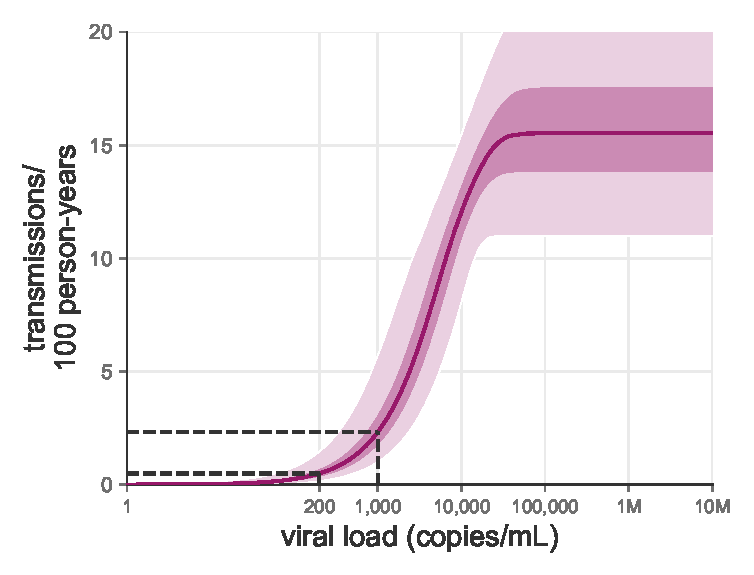
\includegraphics[width=1.0\textwidth]{../figures/eps/intra_couple_trans_risk_ve_artificially_constrained.eps}
  %  \caption{\textbf{HIV transmission in monogamous serodifferent couples, Rakai Community Cohort Study, \protect \var{r1_minYear}-\protect \var{r19_maxYear}, Model \#4. Artificial.} Estimated transmission rate per 100 person-years as a function of index partner viral load assuming that all LLV couples are unlinked except those linked in both p24 and gp41 (R41593$\rightarrow$R64619 and R86742$\rightarrow$R92219). Dotted lines highlight the risk of transmission among donors with low-level viremia (200-1,000 copies/mL). Median value is shown as the central line and shading represents the 95\% and 50\% credible interval. }
 %   \label{fig:intra_couple_trans_risk_artificially_constrained} % Used for referencing
%\end{figure}
%\newpage


%\begin{figure}[!ht] 
   % \centering
  %  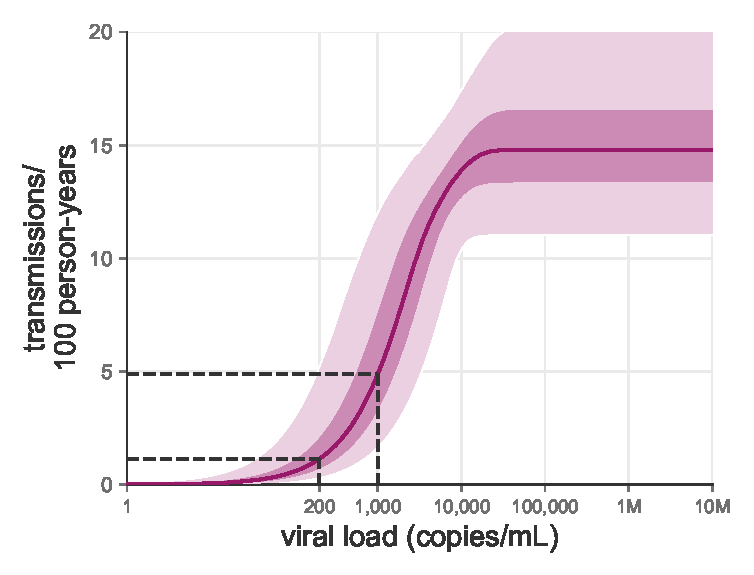
\includegraphics[width=1.0\textwidth]{../figures/eps/intra_couple_trans_risk_ve_unconstrained.eps}
 %   \caption{\textbf{HIV transmission in monogamous serodifferent couples, Rakai Community Cohort Study, \protect \var{r1_minYear}-\protect \var{r19_maxYear}, Model \#5. No genetic constraints.} Estimated transmission rate per 100 person-years as a function of index partner viral load with a $\text{Half-Normal}(0,0.01)$ prior on the extra-partner transmission rate instead of a genetic linkage informed prior. Dotted lines highlight the risk of transmission among donors with low-level viremia (200-1,000 copies/mL). Median value is shown as the central line and shading represents the 95\% and 50\% credible interval. }
    \label{fig:intra_couple_trans_risk_unconstrained} % Used for referencing
%\end{figure}
%\newpage

%\begin{figure}[!ht] % h! forces the figure to stay "here"
   % \centering
  %  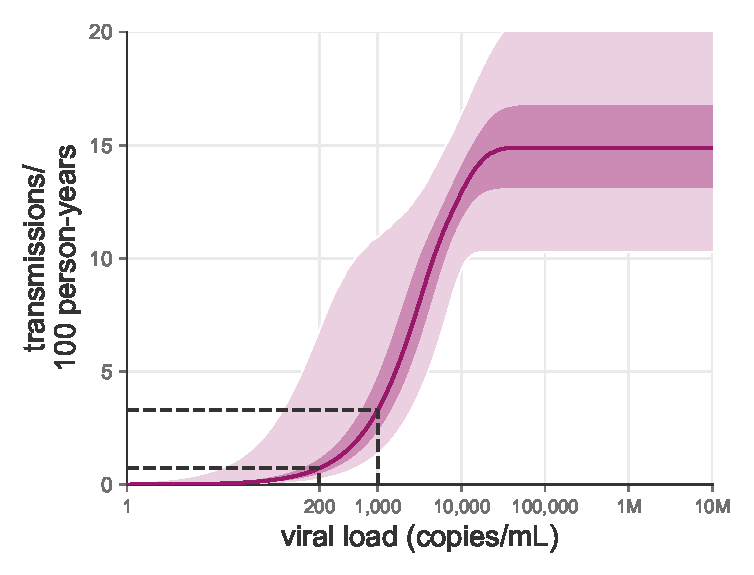
\includegraphics[width=1.0\textwidth]{../figures/eps/intra_couple_trans_risk_ve_constrained_0_1.eps}
 %   \caption{\textbf{HIV transmission in monogamous serodifferent couples, Rakai Community Cohort Study, \protect \var{r1_minYear}-\protect \var{r19_maxYear}, model \#6. Low ART-FN assumption.} Estimated transmission rate per 100 person-years as a function of index partner viral load treating below-detection viral loads due to ART as missing data sampled between 0 and 1 copies/mL instead of between 0 and 40 copies/mL. Dotted lines highlight the risk of transmission among donors with low-level viremia (200-1,000 copies/mL). Median value is shown as the central line and shading represents the 95\% and 50\% credible interval. }
    \label{fig:intra_couple_trans_risk_0_1} % Used for referencing
%\end{figure}
 %\newpage

%\begin{figure}[!ht] % h! forces the figure to stay "here"
   % \centering
  %  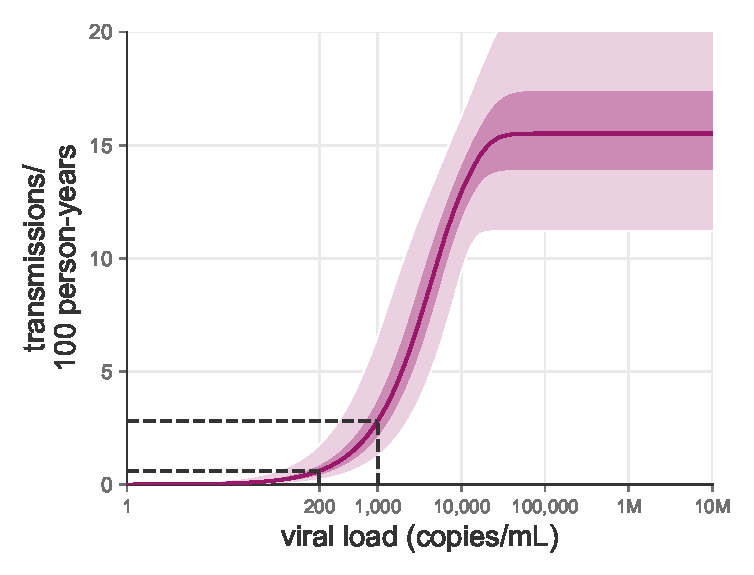
\includegraphics[width=1.0\textwidth]{../figures/eps/intra_couple_trans_risk_ve_constrained_39_40.eps}
 %   \caption{\textbf{HIV transmission in monogamous serodifferent couples, Rakai Community Cohort Study, \protect \var{r1_minYear}-\protect \var{r19_maxYear}, Model \#7. High ART-FN assumption.} Estimated transmission rate per 100 person-years as a function of index partner viral load treating below-detection viral loads as missing data sampled between 39 and 40 copies/mL instead of between 0 and 40 copies/mL. Dotted lines highlight the risk of transmission among donors with low-level viremia (200-1,000 copies/mL). Median value is shown as the central line and shading represents the 95\% and 50\% credible interval. }
    \label{fig:intra_couple_trans_risk_39_40} % Used for referencing
%\end{figure}
 %\newpage

 
% \begin{figure}[!ht] % h! forces the figure to stay "here"
   % \centering
  %  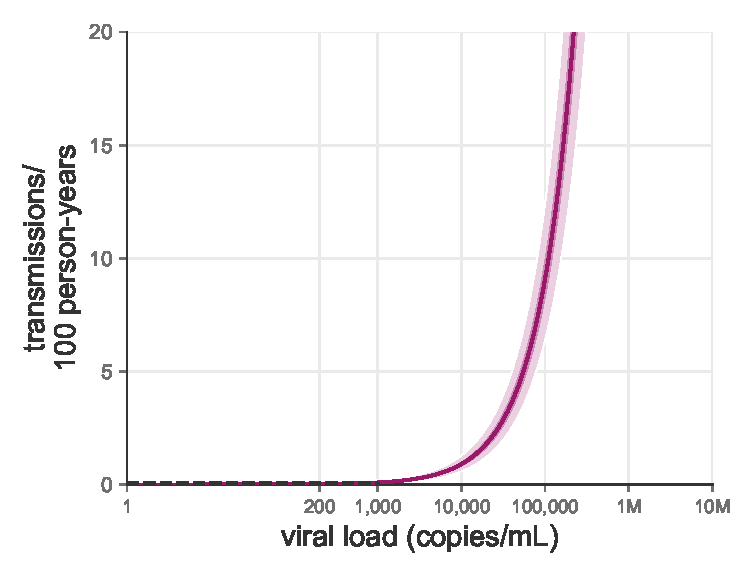
\includegraphics[width=1.0\textwidth]{../figures/eps/intra_couple_trans_risk_ve_nosaturation.eps}
 %   \caption{\textbf{HIV transmission in monogamous serodifferent couples, Rakai Community Cohort Study, \protect \var{r1_minYear}-\protect \var{r19_maxYear}, Model \#8. No saturation .} Estimated transmission rate per 100 person-years as a function of index partner viral load assuming that all sexual acts are ammenable to transmission ($\rho_\text{prod.}=1$). Dotted lines highlight the risk of transmission among donors with low-level viremia (200-1,000 copies/mL). Median value is shown as the central line and shading represents the 95\% and 50\% credible interval. }
    \label{fig:intra_couple_trans_risk_nosaturation} % Used for referencing
%\end{figure}
 %\newpage

 %\begin{figure}[!ht] % h! forces the figure to stay "here"
   % \centering
  %  \includegraphics[width=1.0\textwidth]{../figures/eps/intra_couple_trans_risk_pretreatment.eps}
 %   \caption{\textbf{HIV transmission in monogamous serodifferent couples, Rakai Community Cohort Study, \protect \var{r1_minYear}-\protect \var{r19_maxYear}, Model \#9. Pre-treatment index partners.} Estimated transmission rate per 100 person-years as a function of index partner viral load including only coupling periods between couples with pre-treatment index partners. Dotted lines highlight the risk of transmission among donors with low-level viremia (200-1,000 copies/mL). Median value is shown as the central line and shading represents the 95\% and 50\% credible interval. }
    \label{fig:intra_couple_trans_risk_pretreatment} % Used for referencing
%\end{figure}
 %\newpage

  %\begin{figure}[!ht] % h! forces the figure to stay "here"
   % \centering
  %  \includegraphics[width=1.0\textwidth]{../figures/eps/intra_couple_trans_risk_hill.eps}
 %   \caption{\textbf{HIV transmission in monogamous serodifferent couples, Rakai Community Cohort Study, \protect \var{r1_minYear}-\protect \var{r19_maxYear}, Model \#10. Sigmoidal transmission function.} Estimated transmission rate per 100 person-years as a function of index partner viral load using the sigmoidal transmission functional form. Dotted lines highlight the risk of transmission among donors with low-level viremia (200-1,000 copies/mL). Median value is shown as the central line and shading represents the 95\% and 50\% credible interval. }
    \label{fig:intra_couple_trans_risk_sigmoid} % Used for referencing
%\end{figure}
% \newpage



\clearpage
\bibliographystylesupp{vancouver}
\bibliographysupp{references.bib}

\end{document}
